\documentclass[14pt]{extarticle}

\usepackage{geometry}
\geometry{a4paper,
          total={165mm,257mm},
          left=30mm,
          top=20mm,
         }

% \documentclass{article}

\usepackage[utf8]{inputenc}
\usepackage[T1, T2A]{fontenc}
\usepackage[english, russian]{babel}
\usepackage{csquotes}

\usepackage[
    backend = biber,
    style = numeric,
]{biblatex}

\addbibresource{Refs.bib}

\usepackage{graphicx}
\graphicspath{ {./images/} }

% \usepackage[table,xcdraw]{xcolor}

\usepackage{cmap}

\usepackage{hyperref}
\hypersetup{
    colorlinks=true,
    linkcolor=blue,
    filecolor=blue,
    urlcolor=blue,
    citecolor=blue,
    pdftitle={Отчёт о моделировании частотных сканов},
    pdfpagemode=UseOutlines,
    % pdfstartview={FitB}
}
\urlstyle{same}


\title{Моделирование частотных сканов}
\author{Богачёв А.М.}
\date{\today}


\begin{document}

    \maketitle

    \begin{abstract}
        В отчёте приведены результаты исследований...
    \end{abstract}

    \newpage
    \tableofcontents

    \section{Введение}
Релаксационная спектроскопия глубоких уровней (РСГУ) -- метод исследования 
электрически активных дефектов в полупроводниковых материалах. Данный метод 
обладает высокой чувствительностью к малым концентрациям ловушек носителей 
зарядов и является спектроскопическим. Существуют различные вариации РСГУ, 
например токовая и емкостная, так метод емкостной релаксационной спектроскопии 
глубоких уровней основан на исследовании процесса (сигнала) релаксации ёмкости 
барьерной структуры. Определив значения постоянной времени сигнала релаксации 
для разных температур образца, исследователь может определить энергию активации 
дефекта, вызывающего релаксацию. 

В идеальном случае релаксация ёмкости носит экспоненциальный характер, однако 
так бывает не всегда. Согласно обзору \cite{istratov_exp_analysis} 
сигналы релаксации ёмкости барьерных структур можно условно разделить на три 
группы:
    \begin{enumerate}
        \item Моноэкспоненциальный сигнал релаксации, обусловленный одним 
        единственным энергетическим уровнем в запрещённой зоне полупроводника.
        \item Сигнал релаксации, состоящий из суммы нескольких 
        моноэкспоненциальных сигналов релаксации.
        \item Сигнал релаксации, характеризуемый непрерывным распределением 
        скоростей эмиссии, представленным спектральной функцией $g(\lambda)$.
    \end{enumerate}
В последних двух случаях сигнал не является экспоненциальным. 

Задача определения постоянной времени одной или нескольких экспоненциальных 
составляющих процесса релаксации ёмкости или спектральной функции $g(\lambda)$ 
отностися к задачам экспоненциального анализа. Подходы к решению таких задач,
а также фундаментальные ограничения и особенности сбора и обработки 
экспериментальных данных рассмотрены в исчерпывающем обзоре 
\cite{istratov_exp_analysis}.

Во Владимирском Государственном университете создан измерительно-вычислительный
комплекс релаксационной спектроскопии глубоких уровней, основным измерительным
прибором которого служит спектрометр DLS"~82E фирмы Semilab. 
Измерительно-вычислительный комплекс реализует метод емкостной РСГУ с частотным
сканированием при постоянной температуре. В спектрометре аппаратно реализована
корреляционная обработка сигнала релаксации с опорной функцией lock-in. 

Технические решения, заложенные в названном измерительном оборудовании, требуют
особых методов анализа полученных экспериментальных данных, в частности,
разработки и идентификации моделей частотных сканов (экспериментальных данных, 
полученных на измерительно-вычислительном комплексе).

В следующих разделах отчёта будут рассмотрены модели частотных сканов, некоторые
технические и методические вопросы их реализации и идентификации, а также их
аппробация на экспериментальных данных.

% В современной учебной и технической литературе набирают популярность термины 
% <<машинное обучение>> и <<статистическое обучение>> (например в книгах 
% \cite{hands_on_ml}, \cite{nikolenko_deep_learning}, 
% \cite{elements_of_statistical_learning}). За ними, как правило, скрывается
% процесс создания моделей, которые после идентификации их параметров на некой
% тренировачной выборке (экспериментальных данных с известными целевыми 
% значениями), способны с некоторой точностью определять целевые значения для
% новых, ранее невстречавшихся данных. Таким образом, регрессия и классификация
% являются одними из самых частых задач машинного обучения \cite{hands_on_ml}.
% В данном отчёте термин <<машинное обучение>> будет использоваться именно для 
% обозначения процесса разработки и идентификации моделей, решения задачи 
% регрессии.

    \section{Математические модели частотных сканов}
    В данном разделе представленны описания математических моделей сигнала
    релаксации ёмкости и моделей частотного скана.


    \subsection{Модель сигнала релаксации ёмкости}
    Согласно обзору \cite{istratov_exp_analysis}, зависимость значения
    ёмкости от времени $f(t)$ для моноэкспоненциального сигнала релаксации
    имеет вид выражения \ref{eq:monoexp}.
    \begin{equation}
        \label{eq:monoexp}
        f(t) = A \exp \left(-\lambda t\right) ,
    \end{equation}
    где
    \begin{description}
        \item[\(A\)] -- амплитуда сигнала релаксации ёмкости;
        \item[\(\lambda\)] -- скорость экспоненциального спада,
        обратнопрпорциональная постоянной веремени сигнала релаксации
        $\tau$ (выражение \ref{eq:lambda}).
    \end{description}
    \begin{equation}
        \label{eq:lambda}
        \lambda = \tau ^ {-1}
    \end{equation}
    Спектр моноэкспоненциального сигнала релаксации имеет вид, 
    представленный на рисунке \ref{pic:monoexp_spect_example}.
    \begin{figure}[!ht]
        \centering
        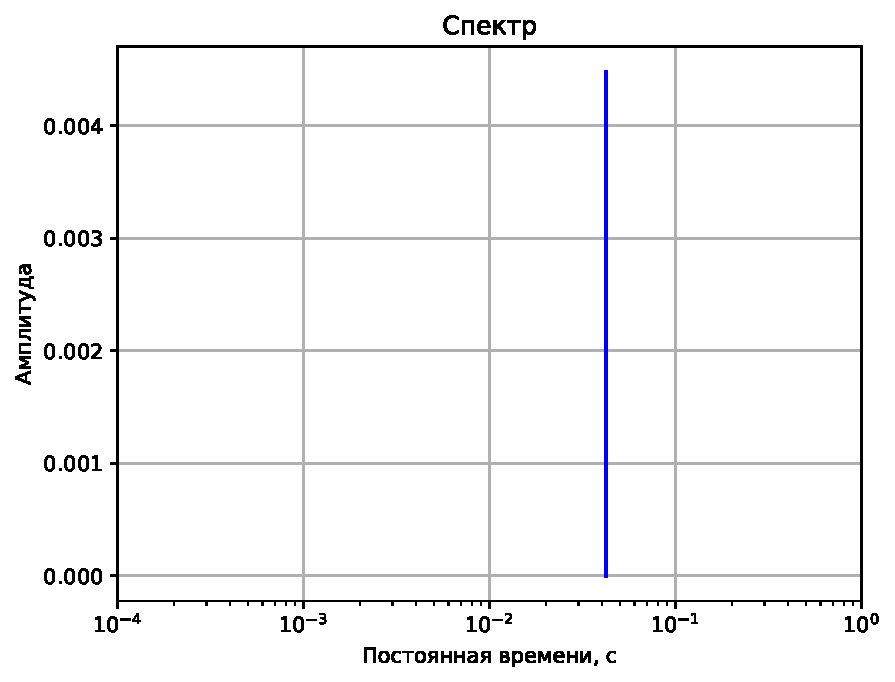
\includegraphics[width=0.5\textwidth]{monoexp_spect_expample}
        \caption{Пример спектра моноэкспоненциального сигнала релаксации
        ёмкости.}
        \label{pic:monoexp_spect_example}
    \end{figure}

    Согласно источнику \cite{istratov_exp_analysis}, зависимость сигнала 
    релаксации ёмкости от времени $f(t)$ для сгинала, образованного 
    несколькими дискретными экспоненциальными сигналами, определяется 
    выражением 
    \ref{eq:discr_multiexp}.
    \begin{equation}
        \label{eq:discr_multiexp}
        f(t) = \sum_{i=1}^{n}A_i\exp\left(-\lambda_i t\right) ,
    \end{equation}
    где $n$ -- количество экспоненциальных составляющих в спектре.
    Пример спектра такого сигнала показан на рисунке 
    \ref{pic:multiexp_spect_example}.
    \begin{figure}[!ht]
        \centering
        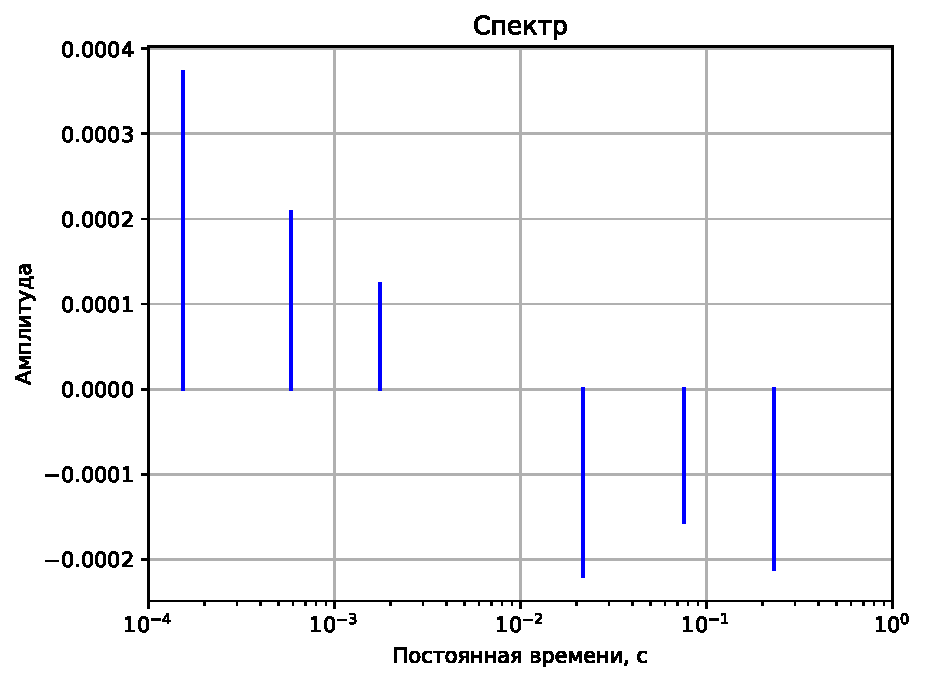
\includegraphics[width=0.5\textwidth]{multiexp_spect_example}
        \caption{Пример спектра сигнала релаксации ёмкости, содержащего
        несколько экспоненциальных составляющих.}
        \label{pic:multiexp_spect_example}
    \end{figure}


    \subsection{Модель идеального частотного скана}
    Предполагается, что в идеальном случае сигнал релаксации ёмкости содержит 
    одну экспоненциальную составляющую, а измерительный тракт спектрометка
    линеен. В таком случае модель частотного скана описывает аппаратные 
    преобразования спектрометра DLS"~82E учитывая только форму его опорной
    функции.

    В спектрометре DLS-82E реализована корреляционная обработка сигнала
    релаксации ёмкости, таким образом сигнал на выходе аналогового тракта
    спектрометра определяется выражением \ref{eq:dlts_correlation_tech},
    согласно публикации \cite{istratov_exp_analysis}.
    \begin{equation}
        \label{eq:dlts_correlation_tech}
        S\left[g(\lambda),t_c,t_d\right]=\frac{1}{t_c}\int_{t_d}^{t_d+t_c}
        f(t)W\left(t-t_d\right)dt ,
    \end{equation}
    где
    \begin{description}
        \item[$W(t)$] -- весовая функция, определённая на интервале 
        времени $\left[0,t_c\right]$,
        \item[$t_c$] -- период (длительность) весовой функции $W(t)$,
        \item[$t_d$] -- время задержки между началом сигнала релаксации
        и началом корреляционной обработки. Согласно обзору 
        \cite{istratov_exp_analysis}, время задержки $t_d$, обычно, 
        вводится для улучшения избирателности или для снижения искажения
        сигнала из-за перегрузки измерительной системы.
        \item[$g(\lambda)$] -- распределение скоростей экспоненциальных
        спадов, составляющих релаксационный сигнал.
    \end{description}

    Модель аппаратных преобразований (корреляционной обработки),
    учитывающая форму весовой функции, реализованной в спектрометре
    DLS"~82E, для моноэкспоненциального сигнала определяется выражением
    \ref{eq:dls82e_model_S} \cite{rp_vak}.
    \begin{equation}
        \label{eq:dls82e_model_S}
        S\left(\tau,C_A,F_0, t_1\right) = C_A K_{BS} K_{LS} 
        \phi\left(\tau,F_0,t_1\right),
    \end{equation}
    где
    \begin{description}
        \item[$C_A$] -- амплитуда емкостного релаксационного сигнала,
        \item[$K_{BS}$] -- масштабный коэффициент, зависящий от 
        чувствительности емкостного моста,
        \item[$K_{LS}$] -- масштабный коэффициент селектора,
        \item[$\tau$] -- постоянная времени релаксации глубокого уровня,
        \item[$F_0$] -- частота сканирования импульсов заполнения,
        \item[$t_1$] -- длительность импульса заполнения,
        \item[$\phi\left(\tau,F_0,t_1\right)$] -- функция определяемая
        выражением \ref{eq:dls82e_model_phi}.
    \end{description}
    \begin{equation}
        \label{eq:dls82e_model_phi}
        \phi\left(\tau,F_0,t_1\right) = 
        M \tau F_0 e^{-\frac{0.05}{\tau F_0}}
        \left(1-e^{\frac{t_1 F_0-0.45}{\tau F_0}}
        -e^{-\frac{0.5}{\tau F_0}}+
        e^{\frac{t_1 F_0-0.95}{\tau F_0}}\right),
    \end{equation}
    где $M$ -- масштабный множитель.

    Масштабный множитель $M$ определяется выражением
    \ref{eq:dls82e_model_M}.
    \begin{equation}
        \label{eq:dls82e_model_M}
        M(\tau, F_0, t_1) = \frac{1}{\max{\left[
        \tau F_0 e^{-\frac{0.05}{\tau F_0}}
        \left(1-e^{\frac{t_1 F_0-0.45}{\tau F_0}}
        -e^{-\frac{0.5}{\tau F_0}}+
        e^{\frac{t_1 F_0-0.95}{\tau F_0}}\right)
        \right]}}
    \end{equation}

    Введём коэффициент $A$ (выражение \ref{eq:dls82e_model_A}), 
    характеризующий амплитуду сигнала релаксации ёмкости и перепишем 
    выражение \ref{eq:dls82e_model_S} с учётом того, что длительность
    импульса заполнения $t_1$ является неизменной величиной, и получим
    выражение \ref{eq:dls82e_model_S_short}.
    \begin{equation}
        \label{eq:dls82e_model_A}
        A = C_A K_{BS} K_{LS}.
    \end{equation}
    \begin{equation}
        \label{eq:dls82e_model_S_short}
        S(\tau,A,F_0) = A\phi(\tau, F_0)
    \end{equation}


    \subsection{Модель, учитывающая нелинейность и неэкспоненциальность}

    Для одновременного учёта нелинейности аппаратного тракта и 
    неэкспоненциальности сигнала релаксации, связанной с присутствием 
    нескольких экспоненциальных составляющих в модель вводят коэффициент
    нелинейности"=неэкспоненциальности $p$ \cite{rp_vak}, после чего 
    выражение \ref{eq:dls82e_model_S_short} приобретает вид выражения 
    \ref{eq:dls82e_model_S_p}.
    \begin{equation}
        \label{eq:dls82e_model_S_p}
        S(\tau,A,F_0,p) = A\left[\phi(\tau, F_0)\right]^p.
    \end{equation}

    В случае моноэкспоненциального сигнала релаксации и линейного измерительного
    тракта коэффициент $p=1$, в остальных случаях он отклоняется от 1. Данный 
    коэффициент комплексно учитывает нелинейность и неэкспоненциальность, что
    позволяет повысить точность моделирования, но он не позволяет дать ответ 
    на вопрос какой именно из этих двух факторов имел место.


    \subsection{Модель многоэкспоненциального частотного скана}
    Если предположить, что сигнал релаксации ёмкости состоит из нескольких
    экспоненциальных составляющих и определяется выражением
    \ref{eq:discr_multiexp}, то опираясь на выражения
    \ref{eq:discr_multiexp}, \ref{eq:dlts_correlation_tech}, 
    \ref{eq:dls82e_model_S_short} и \ref{eq:dls82e_model_phi}, можно
    сделать выод, что частотный скан, созданный таким сигналом релаксации
    ёмкости определяется выражением~\ref{eq:multiexp_frequncy_scan}.
    \begin{equation}
        \label{eq:multiexp_frequncy_scan}
        Y = \sum_{i=1}^{n} A_i \phi(\tau_i, F_0) ,
    \end{equation}
    где $n$ -- количество экспоненциальных составляющих в сигнале 
    релаксации.
    Данная модель предполагает, что измерительный такт линеен.

    \section{Реализация моделей}
	В данном разделе приводится краткое описание программной реализации
	моделей, примеры рассчитанных частотных сканов, примеры результатов
	идентификации их моделей, рассматриваются некоторые методические вопросы.


	\subsection{Интерфейс и функционал}
	Модели оформлены в виде пакета модулей на языке программирования Python~3.
	Интерфейс моделей совместим с одной из самых популярных библиотек для 
	машинного обучения scikit-learn \cite{sklearn_website}. Такое техническое
	решение позволяет использовать имеющиеся в библиотеке инструменты 
	предобработки данных, оценки качества и оптимизации параметров 
	моделей, а также интегрировать модели в друге программное обеспечение и 
	конвейеры обработки данных.

	Разработанные модели (выражения	\ref{eq:dls82e_model_S_short}, 
	\ref{eq:dls82e_model_S_p}, \ref{eq:multiexp_frequncy_scan}), выполняют две 
	функции:
	\begin{enumerate}
		\item Вычисление частотного скана с заданными параметрами.
		\item Идентификация параметров модели частотного скана по 
		экспериментальным данным.
	\end{enumerate}
	Идентификация параметров моделей реализована методом градиентного спуска.
	Имеется возможность вывода значений параметров модели на каждой итерации.
	Реализована автоматическая остановка идентификации при достижении заданного
	модуля разницы между значениями функции потерь на текущей и предыдущей 
	итерации.

	Модели реализуют единообразный интерфейс. При инициализации каждая модель 
	получает длительность импульса заполнения (параметр filling\_pulse),
	которая считается неизменной при измерениях) и параметры алгоритма 
	идентификации. Параметры алгоритма идентификации варьируются:
	\begin{itemize}
		\item модель идеального частотного скана и модель частотного скана с 
		показателем нелинейности-неэкспоненциальности (выражения 
		\ref{eq:dls82e_model_S_short}, \ref{eq:dls82e_model_S_p}): 
			\begin{description}
				\item[fit\_p\_coef] -- если параметр принимает значение True 
				(логическую единицу), тогда при идентификации параметров модели
				определяется показатель нелинейности-неэкспоненциальности $p$,
				иначе (False -- логический ноль) $p$ считается равным 1 и не 
				изменяется при идентификации параметров модели;
				\item[learning\_rate] -- скорость градиентного спуска;
				\item[n\_iters] -- максимальное количесво итераций при 
				идентификации;
				\item[stop\_val] -- модуль разницы между значениями функции 
				потерь на текущей и предыдущей итерации, при достижении которого
				происходит остановка идентификации;
				\item[verbose] -- если параметр принимает значение True, то в 
				стандартный поток вывода печатаются значения параметров модели
				на каждой итерации.
			\end{description}

		\item модель многоэкспоненциального частотного скана (выражение 
		\ref{eq:multiexp_frequncy_scan}):
			\begin{description}
				\item[n\_exps] -- количество экспоненециальных составляющих в 
				сигнале релаксации (значение $n$ в выражении 
				\ref{eq:multiexp_frequncy_scan});
				\item[learning\_rate] -- скорость градиентного спуска;
				\item[n\_iters] -- максимальное количесво итераций при 
				идентификации;
				\item[stop\_val] -- модуль разницы между значениями функции 
				потерь на текущей и предыдущей итерации, при достижении которого
				происходит остановка идентификации;
				\item[verbose] -- если параметр принимает значение True, то в 
				стандартный поток вывода печатаются значения параметров модели
				на каждой итерации.
			\end{description}
	\end{itemize}

	При идентификации параметров модели идеального частотного скана 
	определяется амплитуда и десятичный логарифм постоянной времени 
	($\log_{10}(\tau)$) сигнала релаксации. Причины замены постоянной времени
	её десятичном логарифмом объясняются в следующем разделе.

	При идентификации модели с показателем нелинейности"=неэкспоненциальности
	к амплитуде и десятичному логарифму постоянной времени сигнала релаксации
	добавляется значение показателя нелинейности"=неэкспоненциальности $p$.

	При идентификации многоэкспоненциальной модели определяется $n$ пар 
	амплитуда --- десятичный логарифм постоянной времени сигнала релаксации. 
	По паре для каждой из $n$ экспоненциальных составляющих.

	Параметры модели частотного скана могут быть не только идентифицированны,
	но и заданы пользователем.

	Чтобы выполнить идентификацию параметров модели, нужно передать ей 
	набор экспериментальных (тренировачных) данных, состоящих из вектора 
	значений десятичных логарифимов частоты опорной функции ($\log_{10}(F_0)$)
	и соответствующего вектора значений сигнала DLTS -- сигнала на выходе 
	аппаратного тракта спектрометра DLS-82E. При идентификации параметров модели
	по умолчанию их начальные параметры выбираются случайным образом, однако
	могут быть и определены пользователем.

	При идентификации модели значения её параметров на каждой итерации 
	сохраняются в атрибуте fit\_results\_, что позволяет пользователю
	получить и проанализировать данные о работе алгоритма идентификации.

	При вычислении частотного скана с заданными параметрами модели передаётся
	вектор значений десятичных логарифимов частоты опорной функции, для каждого 
	из которых модель вычислит значение сигнала	DLTS.


	\subsection{Алгоритм идентификации параметров моделей}
	Идентификация параметров модели производится методом градиетного 
	спуска, при этом минимизируется среднеквадратическая ошибка между 
	значениями, полученными в результате измерений, и результатами 
	моделирования (выражение \ref{eq:mse}).
	\begin{equation}
		\label{eq:mse}
		E = \frac{1}{m}\sum_{i=1}^{m}\left(y_i - y_i^*\right)^2,
	\end{equation}
	где
	\begin{description}
		\item[$y_i$] -- значения, полученные в результате измерений,
		\item[$y_i^*$] -- значения, полученные в результате моделирования,
		\item[$m$] -- количество измерений.
	\end{description}
	При каждом обновлении постоянной времени сигнала релаксации (как при 
	идентификации модели, на каждой итерации, так и при обновлении постоянной 
	времени пользователем) вычисляется масштабный множитель $M(\tau, F_0, t_1)$, 
	определяемый выражением \ref{eq:dls82e_model_M}. Таким образом модель 
	всякий раз вычисляет значение 	
	\(
		\max{\left[
	    \tau F_0 e^{-\frac{0.05}{\tau F_0}}
	    \left(1-e^{\frac{t_1 F_0-0.45}{\tau F_0}}
	    -e^{-\frac{0.5}{\tau F_0}}+
	    e^{\frac{t_1 F_0-0.95}{\tau F_0}}\right)
	    \right]}
    \).
    В текущей реализации моделей данный максимум вычисляется приблизительно
    с помощью градиентного спуска. Не смотря на то, что применяемый итеративный
    алгоритм находит максимум очень быстро, эти вычисления занимают довольно 
    много веремени при идентификации моделей, потому что выполняются на 
    каждой итерации (при каждом обновлений постоянной времени $\tau$). В случае 
    многоэкспоненциальной модели данный процесс повторяется еще и для каждой 
    экспоненциальной составляющей, что заметно снижает скорость идентификации 
    модели при значениях параметра n\_exps больше 10. Таким образом в будущем 
    вычисления можно будет оптимизировать за счёт одного из следющих решений:
    \begin{enumerate}
    	\item найти точное аналитическое выражение для расчёта 
    	$M(\tau, F_0, t_1)$,
    	\item найти для $M(\tau, F_0, t_1)$ аппроксимирующую функцию, 
    	позволяющую вычислять мастабный множитель с приемлимой точностью.
    \end{enumerate}

	В моделях градиентный спуск реализован при помощи библиотеки TensorFlow
	\cite{tf_website}, главное преимущество которой в том, что она реализует
	алгоритм автоматического дифференцирования на графе вычислений. Таким 
	образом, при расчёте градиентов сначала производные берутся символьно 
	(точно), а затем вычисляются их значения, поэтому точность вычисления 
	градиента ограничена только разрядностью чисел \cite{hands_on_ml},
	\cite{nikolenko_deep_learning}, \cite{tf_website}.

	Во всех моделях используется алгоритм идентификации с постоянной и одинаковой
	для всех параметров скроростью градиентного спуска, поэтому для ускорения 
	идентификации параметров моделей и улучшения сходимости алгоритма необходима 
	нормализация (прведение к единому масштабу) тренировочных данных.
	
	\begin{figure}[!htp]
		\centering
		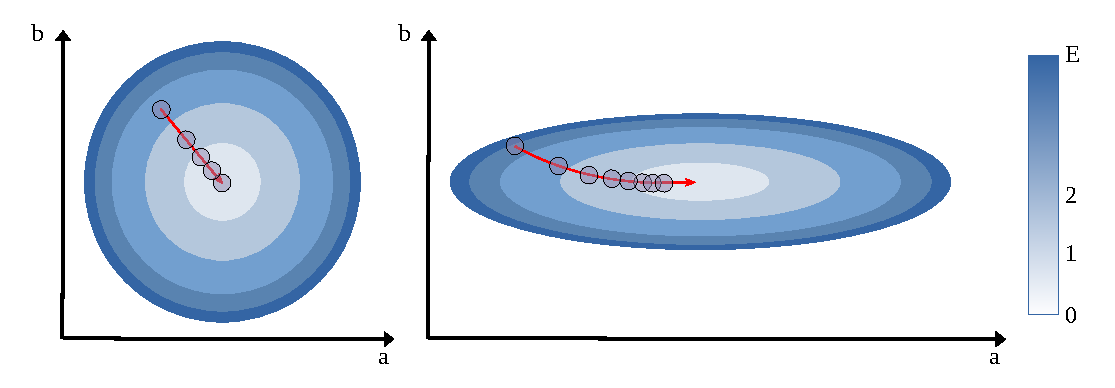
\includegraphics[width=\textwidth]{path_example}
		\caption{Градиентный спуск с нормализацией тренировачных данных (график
		слева) и без неё (график справа) для модели с двумя параметрами. $a$ и 
		$b$ -- параметры модели, $E$ -- функция потерь.}
		\label{pic:path_example}
	\end{figure}

	Рассмотрим примеры на рисунке \ref{pic:path_example}. В идеальном случае 
	функция потерь (среднеквадратическая ошика -- выражение \ref{eq:mse}) должна
	иметь форму <<симметричной чаши>>, а изменение обоих параметров должно вносить 
	одинаковый вклад в значение градиента. В таком случае алгоритм градиентного 
	спуска достигнет минимума функции потерь кратчайшим путём, как на левом 
	графике рисунка \ref{pic:path_example}. Если же тренировочные данные имеют
	очень разные масштабы, функция потерь (гафик справа на рисунке 
	\ref{pic:path_example}) будет иметь форму <<вытянутой чаши>>, а алгоритм 
	идентификации будет долго подстраивать одни из параметров без существенного
	изменения функции потерь \cite{hands_on_ml}. Чтобы минимизировать этот 
	эффект,	тренировочные данные нормализуют перед идентификацей параметров 
	модели. После идентификации параметры модели и тренировочные данные можно
	вернуть в исходный масштаб.

	Для разрабатанных моделей тренировочные данные данные имеют существенно
	отличающиеся масштабы: значение сигнала DLTS находятся в диапазоне долей
	пикофарад, а диапазон изменения частоты опорной функции спектрометра
	покрывает три декады (от 1 Гц до 2500 кГц). Таким образом, желательно 
	выполнять нормализацию исходных данных перед идентификацией параметров
	модели. Кроме этого, изменение параметров модели (постоянной времени и 
	амплитуды) вносят существенно различающийся вклад в градиент функции потерь.
	Если снова обратиться к выражениям \ref{eq:dls82e_model_phi} и 
	\ref{eq:dls82e_model_S_short}, можно заметить, что значение функции потерь
	пропорционально первой степени амплитуды $A$ сигнала релаксации и экспоненте,
	возведенной в степень скорости экспоненциального спада, то есть
	$e^\frac{1}{\tau}$. Поэтому на вход моделей при идентификации подаётся 
	десятичный логарифм частоты опорной функции ($\log_{10}(F_0)$), а 
	идентификация производится не по постоянной времени $\tau$, а по десятичному
	логарифму постоянной времени $\log_{10}(\tau)$. На рисунке \ref{pic:path}
	показан приемер идентификации идельного частотного скана. <<Путь>> 
	параметров модели в процессе идентификации показывает красная линия с 
	маркерами, а изолинии и градиент -- значения функции потерь.

    \begin{figure}[!htp]
        \centering
        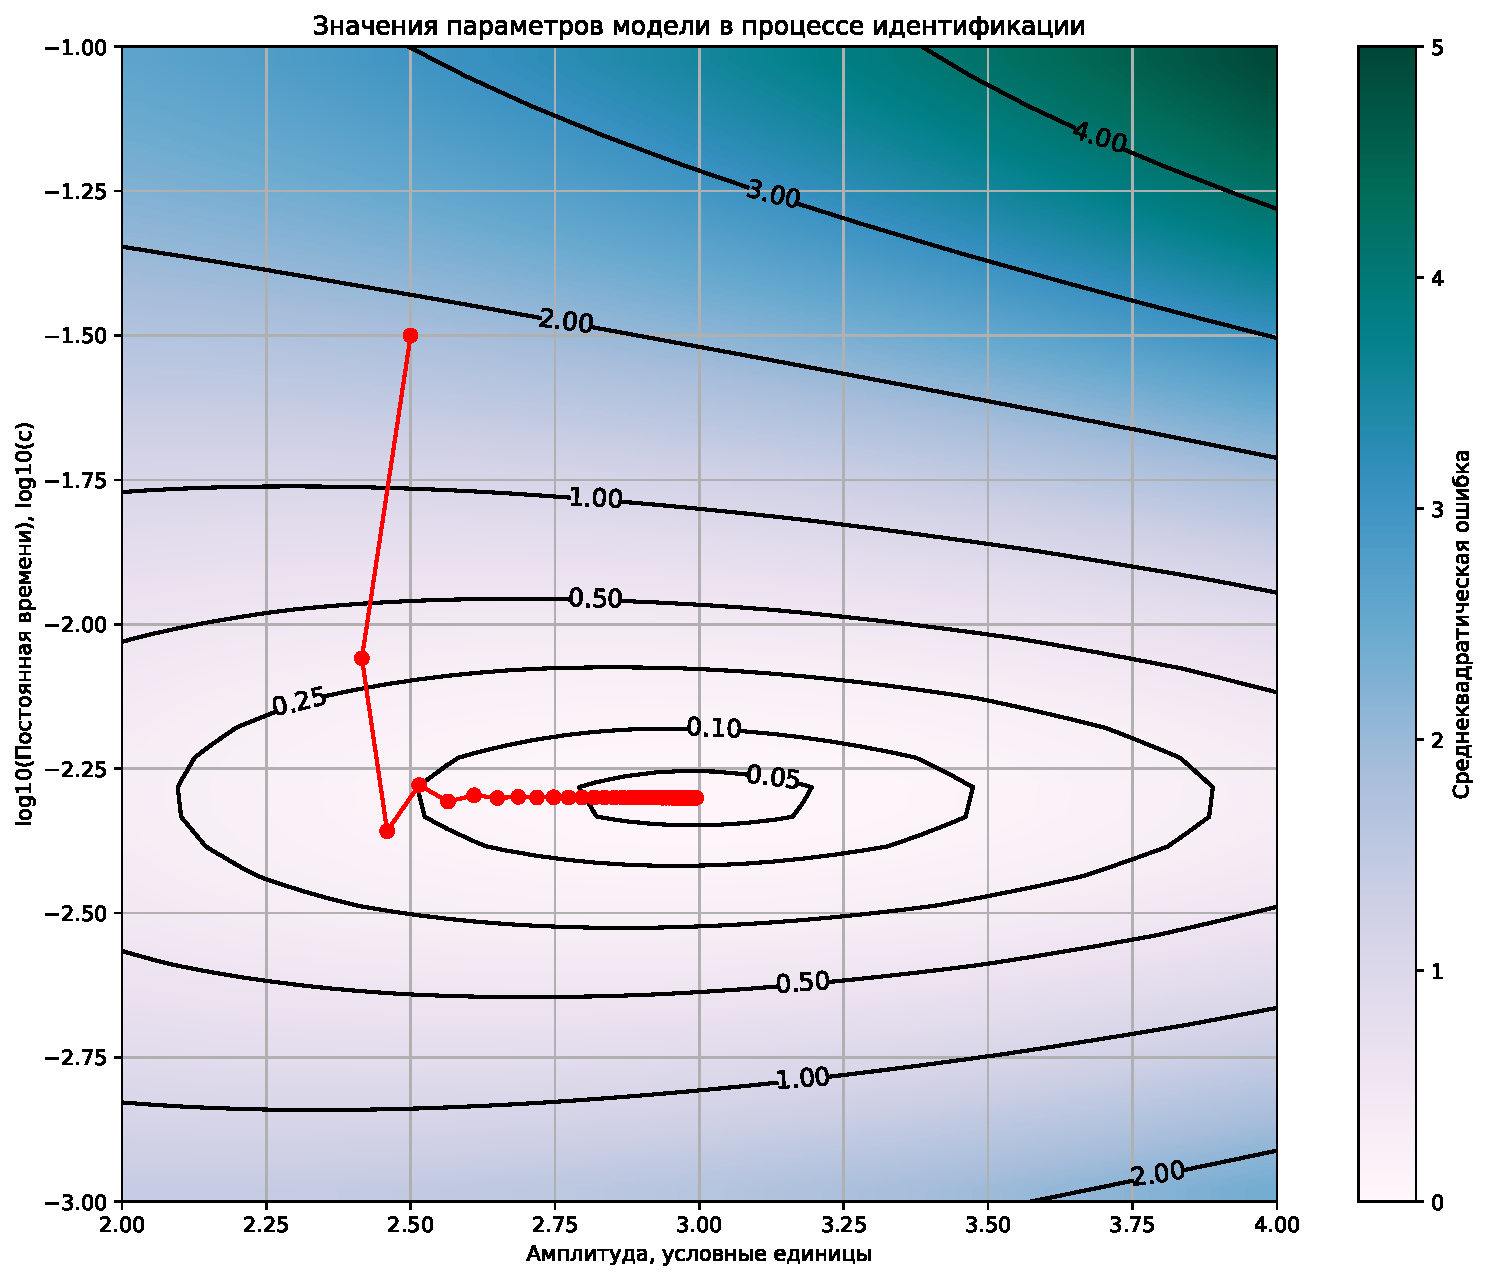
\includegraphics[width=0.75\textwidth]{path}
        \caption{<<Путь>> значений параметров при идентификации.}
        \label{pic:path}
    \end{figure}

    На рисунке \ref{pic:path} форма изолиний отличается от концентрических 
    окружностей, а <<путь>> параметров не похож на прямую линию, что говорит
    о том, что возможна дальнейшая оптимизация алгоритма идентификации, однако,
    названные выше меры позволили значительно смягчить эффект от различных 
    масштабов в экспериментальных данных и в параметрах модели. Также возможно
    использование одного из алгоритмов адаптивного градиентного спуска, то есть
    алгоритмов изменяющих скорость по мере приближения к оптимальным значениям
    параметров. Такое решение не изменит форму функции потерь, но оптимизирует
    <<путь>> и количество итераций.

    Рисунки \ref{pic:identification_test} и \ref{pic:multiexp_test} показывают
    примеры результатов идентификации модели идеального частотного скана и 
    модели многоэкспоненциального частотного скана соответственно на 
    расчитанных тренировочных данных.

    \begin{figure}[!htp]
        \centering
        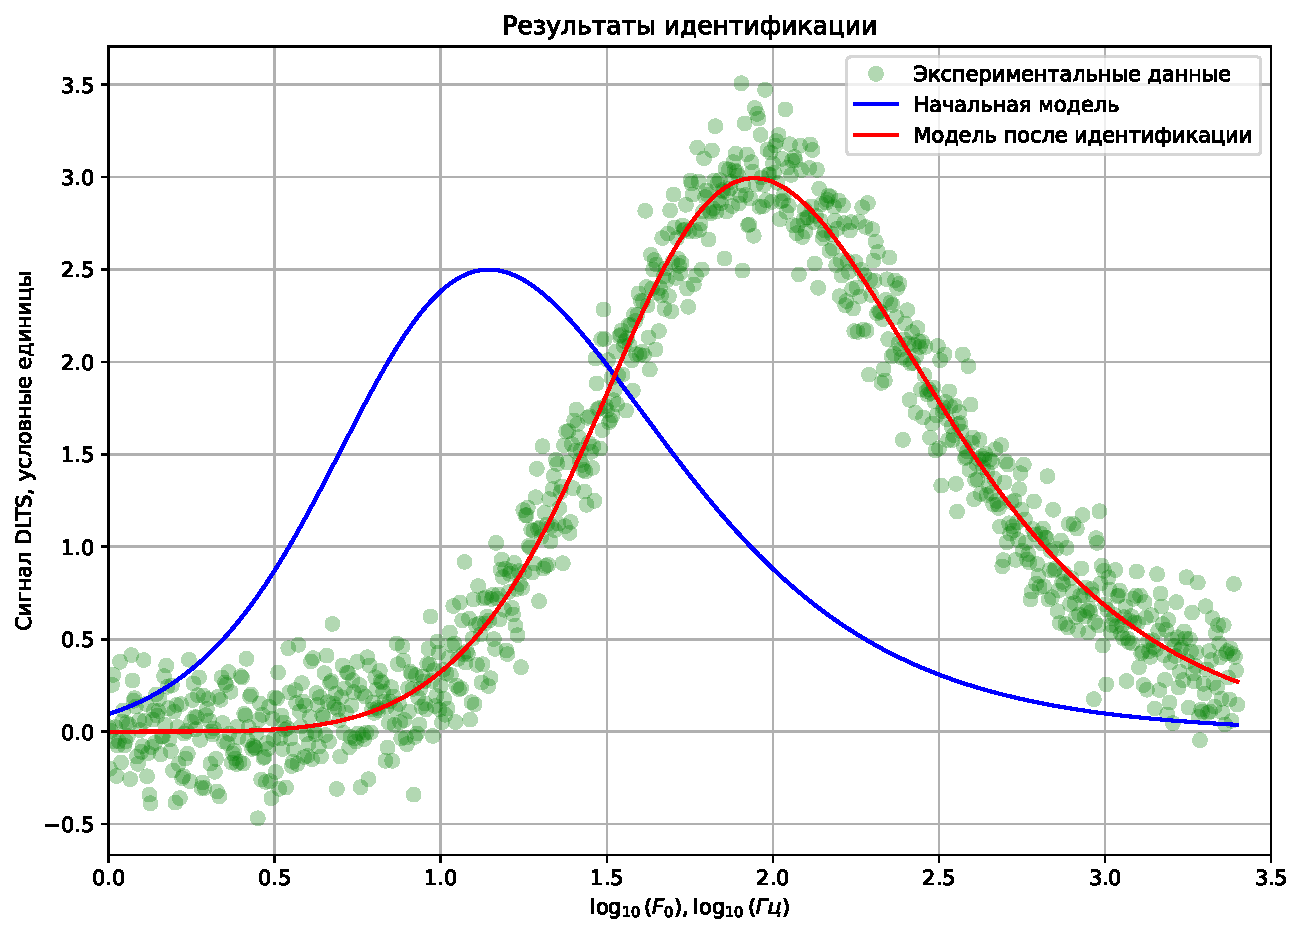
\includegraphics[width=0.75\textwidth]{identification_test}
        \caption{Пример результата идентификации модели идеального частотного 
        скана.}
        \label{pic:identification_test}
    \end{figure}


    \begin{figure}[!htp]
        \centering
        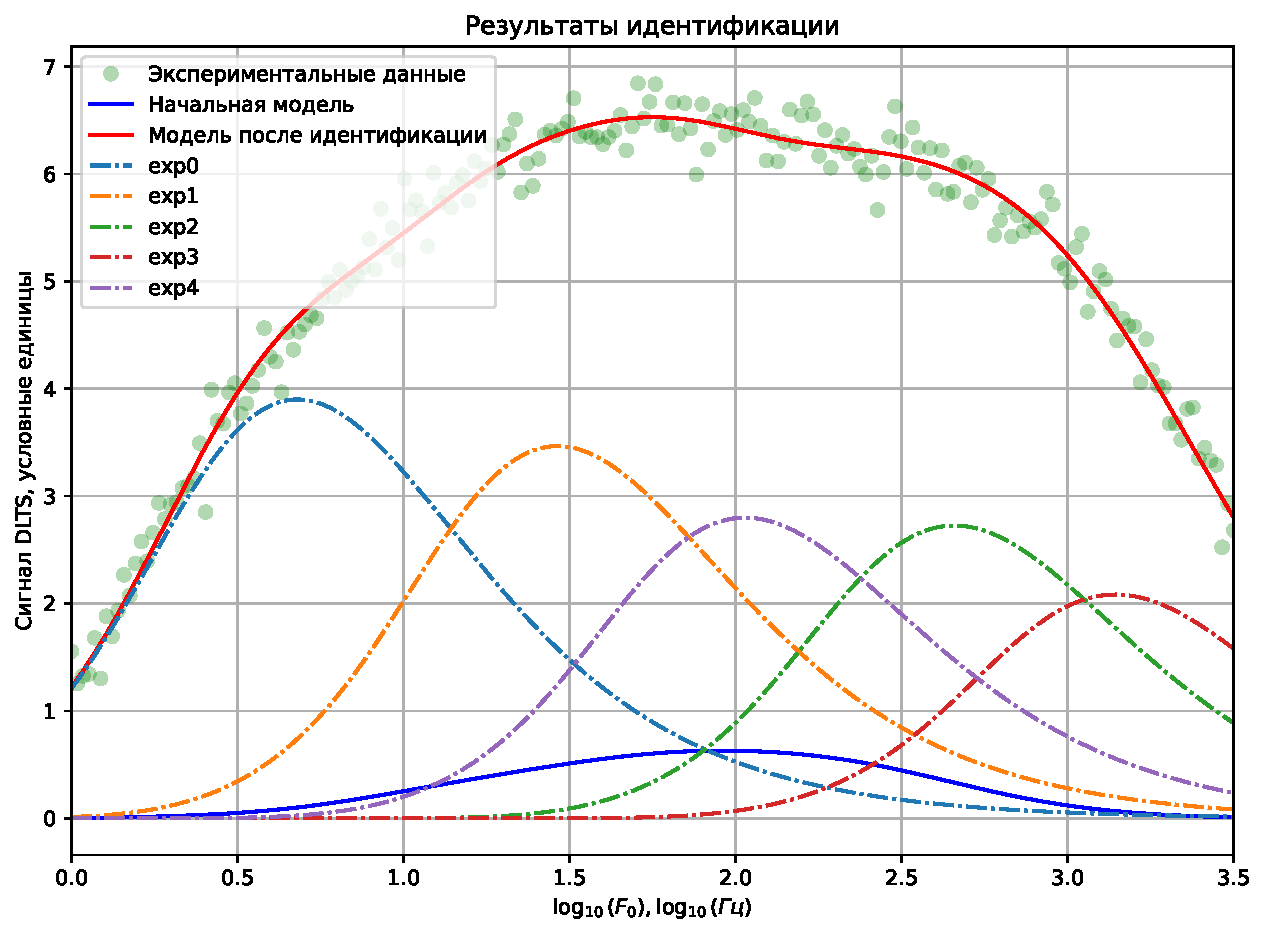
\includegraphics[width=0.75\textwidth]{multiexp_test}
        \caption{Пример результата идентификации модели многоэкспоненциального
        частотного скана. Штрихпунктирными линиями показаны частотные сканы для
        отдельных экспоненциальных составляющих сигнала релаксации.}
        \label{pic:multiexp_test}
    \end{figure}


    \subsection{Оценка качества модели}
    Вычисление корня из среднеквадратической ошибки (англ. root-mean-square 
    error -- RMSE) между экспериментальными данными и данными, полученными с 
    помощью моделирвоания, -- один из самых известных и распространенных 
    способов оценки качества регрессии данных разработанной моделью. Однако, 
    одного этого показателя часто бывает недостаточно, более того, 
    \textbf{оценка этого показателя только на тренировочных данных} при 
    разработке модели (\textbf{особенно эмпирической модели}) -- методическая 
    ошибка \cite{hands_on_ml}, \cite{sklearn_cross_validation}. Данные 
    утверждения обусловлены следующим:
    \begin{itemize}
    	\item сам по себе корень из среднеквадратической ошибки не отвечает на 
    	вопрос о <<фундаментальном>> соответствии данных модели, а также не 
    	показывает какова вероятность того, что полученное значение -- результат 
    	случайного совпадения;
    	\item оценивая данную метрику только на тренировочных данных, есть риск
    	получить слишком оптимистическую оценку и столкнуться с проблемой, 
    	называемой <<оверфитинг>> (от англ. overfitting)\cite{hands_on_ml}, 
    	\cite{sklearn_cross_validation}, \cite{nikolenko_deep_learning}.
    \end{itemize}

    Для начала, для иллюстрации приведённых аргументов обратимся к набору 
    данных, известному под названием <<Квартет Энскомба>>. Это набор данных был 
    создан математематиком Фрэнком Энскомбом специально для того, чтобы показать
    важность визуализации данных в графиках. Особенность этого набора в том, что
    он состоит из четырёх групп данных, имеющих одинаковые статистические 
    характеристики, но абсолютно разные графики \cite{anscombe_quartet_wikipedia}, 
    \cite{anscombe_quartet_article}. Графики приведены на рисунке 
    \ref{pic:anscombe_quartet}, статистические характеристки -- в табилице 
    \ref{table:anscombe_quartet_statistics}.

    \begin{figure}[!htp]
        \centering
        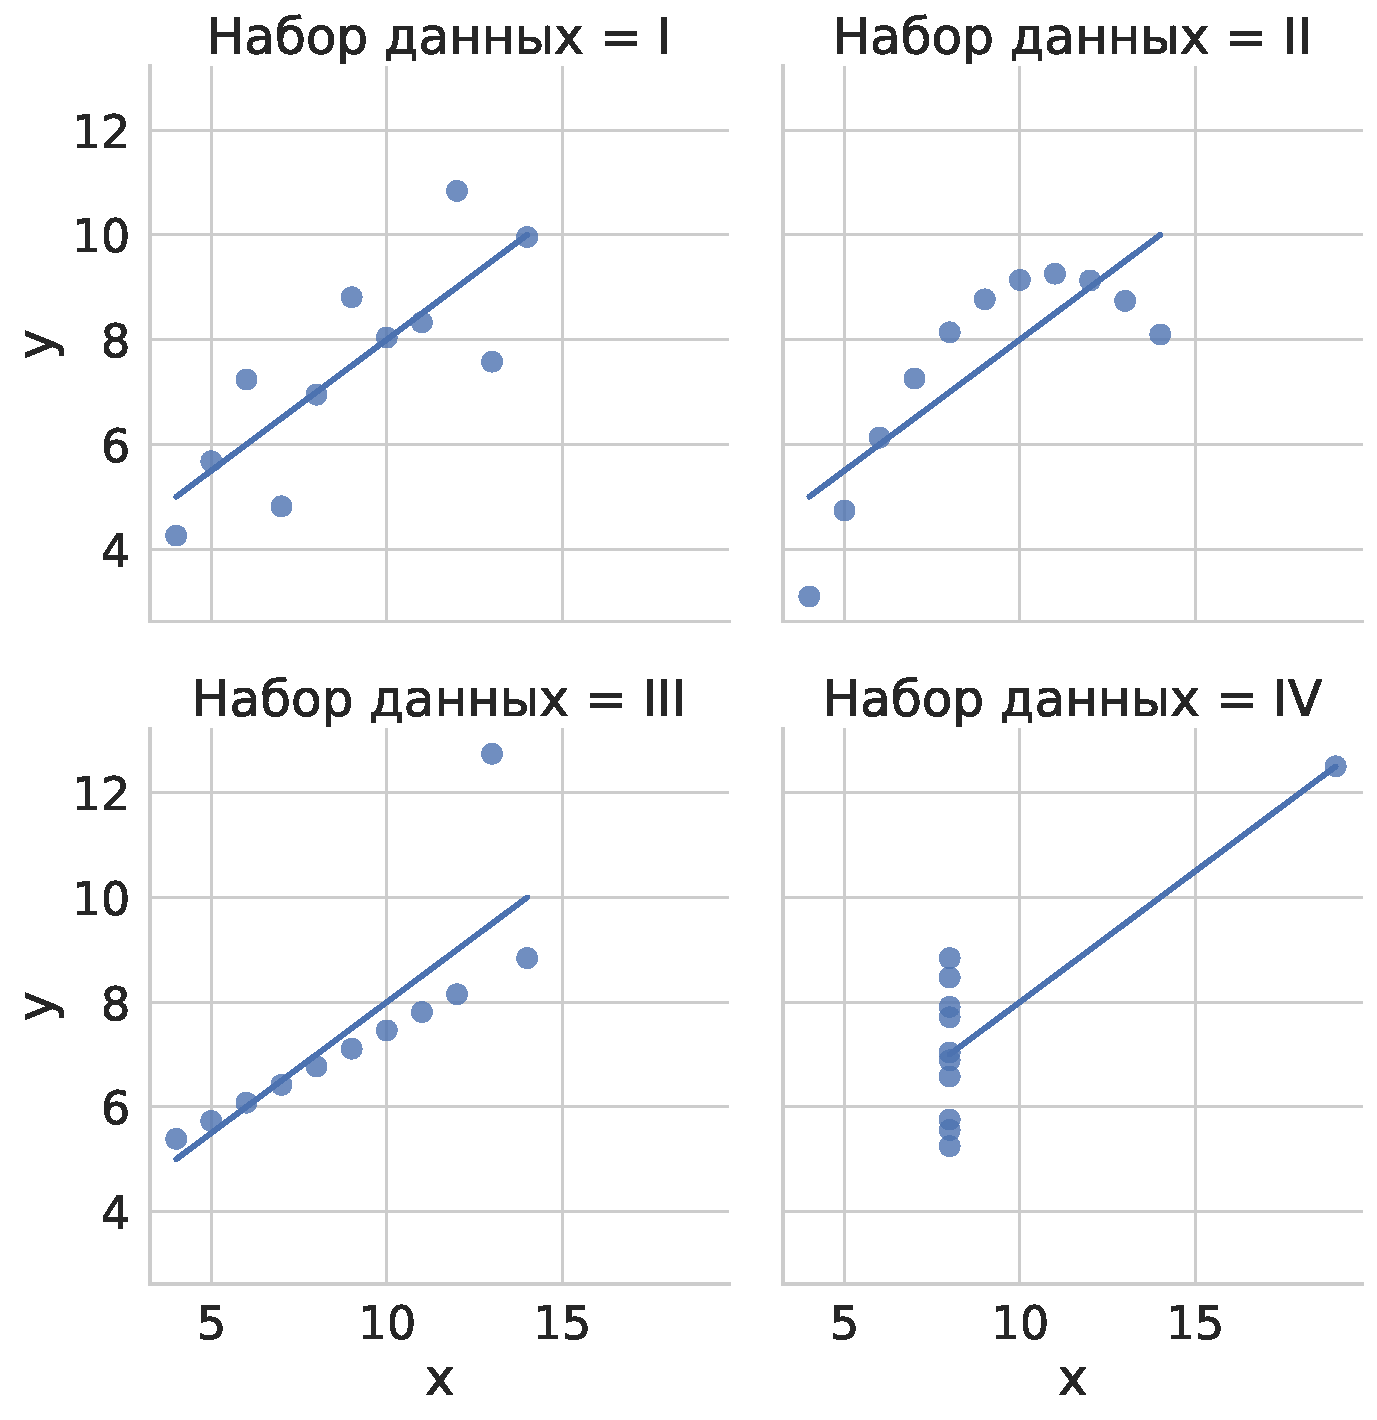
\includegraphics[width=0.7\textwidth]{anscombe_quartet}
        \caption{Квартет Энскомба.}
        \label{pic:anscombe_quartet}
    \end{figure}

    \begin{table}[!htp]
    	\centering
    	\caption{Статистические свойства наборов данных в Квартете Энскомба}
		\begin{tabular}{|l|l|}
			\hline
			Характеристика                         & Значение   \\ \hline
			Среднее значение переменной $x$        & 9.0        \\ \hline
			Дисперсия переменной $x$               & 10.0       \\ \hline
			Среднее значение переменной $y$        & 7.5        \\ \hline
			Дисперсия переменной $y$               & 3.75       \\ \hline
			Корреляция между переменными $x$ и $y$ & 0.816      \\ \hline
			Уравнение линейной регрессии           & $y=3+0.5x$ \\ \hline
			Коэффициент детерминации               & 0.67       \\
			линейной регрессии ($R^2$)             &            \\ \hline
		\end{tabular}
		\label{table:anscombe_quartet_statistics}
	\end{table}

	Что примечательно, все 4 подгруппы данных имеют одно и то же урванение 
	линейной регрессии (см. таблицу \ref{table:anscombe_quartet_statistics}) и, 
	как показано в таблице \ref{table:anscombe_quartet_rmse}, очень близкие 
	занчения корня из среднеквадратической ошибки.

	\begin{table}[!htp]
    	\centering
    	\caption{Значения корней из среднеквадратической ошибки}
		\begin{tabular}{|l|c|c|c|c|}
			\hline
			Набор данных                        & I     & II    & III   & IV    \\ \hline
			Значение корня среднеквадратической & 1.119 & 1.119 & 1.118 & 1.118 \\ 
			ошибки (RMSE)                       &       &       &       &       \\ \hline
		\end{tabular}
		\label{table:anscombe_quartet_rmse}
	\end{table}

	В таблице \ref{table:anscombe_quartet} для справки приведены данные из 
	<<Квартета Энскомба>>.

    \begin{table}[!htp]
    	\centering
    	\caption{Квартет Энскомба}
		\begin{tabular}{|ll|ll|ll|ll|}
			\hline
			\multicolumn{2}{|c|}{I}                             & \multicolumn{2}{c|}{II}                            & \multicolumn{2}{c|}{III}                           & \multicolumn{2}{c|}{IV}                            \\ \hline
			\multicolumn{1}{|c|}{x}    & \multicolumn{1}{c|}{y} & \multicolumn{1}{c|}{x}    & \multicolumn{1}{c|}{y} & \multicolumn{1}{c|}{x}    & \multicolumn{1}{c|}{y} & \multicolumn{1}{c|}{x}    & \multicolumn{1}{c|}{y} \\ \hline
			\multicolumn{1}{|l|}{10,0} & 8,04                   & \multicolumn{1}{l|}{10,0} & 9,14                   & \multicolumn{1}{l|}{10,0} & 7,46                   & \multicolumn{1}{l|}{8,0}  & 6,58                   \\ \hline
			\multicolumn{1}{|l|}{8,0}  & 6,95                   & \multicolumn{1}{l|}{8,0}  & 8,14                   & \multicolumn{1}{l|}{8,0}  & 6,77                   & \multicolumn{1}{l|}{8,0}  & 5,76                   \\ \hline
			\multicolumn{1}{|l|}{13,0} & 7,58                   & \multicolumn{1}{l|}{13,0} & 8,74                   & \multicolumn{1}{l|}{13,0} & 12,74                  & \multicolumn{1}{l|}{8,0}  & 7,71                   \\ \hline
			\multicolumn{1}{|l|}{9,0}  & 8,81                   & \multicolumn{1}{l|}{9,0}  & 8,77                   & \multicolumn{1}{l|}{9,0}  & 7,11                   & \multicolumn{1}{l|}{8,0}  & 8,84                   \\ \hline
			\multicolumn{1}{|l|}{11,0} & 8,33                   & \multicolumn{1}{l|}{11,0} & 9,26                   & \multicolumn{1}{l|}{11,0} & 7,81                   & \multicolumn{1}{l|}{8,0}  & 8,47                   \\ \hline
			\multicolumn{1}{|l|}{14,0} & 9,96                   & \multicolumn{1}{l|}{14,0} & 8,10                   & \multicolumn{1}{l|}{14,0} & 8,84                   & \multicolumn{1}{l|}{8,0}  & 7,04                   \\ \hline
			\multicolumn{1}{|l|}{6,0}  & 7,24                   & \multicolumn{1}{l|}{6,0}  & 6,13                   & \multicolumn{1}{l|}{6,0}  & 6,08                   & \multicolumn{1}{l|}{8,0}  & 5,25                   \\ \hline
			\multicolumn{1}{|l|}{4,0}  & 4,26                   & \multicolumn{1}{l|}{4,0}  & 3,10                   & \multicolumn{1}{l|}{4,0}  & 5,39                   & \multicolumn{1}{l|}{19,0} & 12,50                  \\ \hline
			\multicolumn{1}{|l|}{12,0} & 10,84                  & \multicolumn{1}{l|}{12,0} & 9,13                   & \multicolumn{1}{l|}{12,0} & 8,15                   & \multicolumn{1}{l|}{8,0}  & 5,56                   \\ \hline
			\multicolumn{1}{|l|}{7,0}  & 4,82                   & \multicolumn{1}{l|}{7,0}  & 7,26                   & \multicolumn{1}{l|}{7,0}  & 6,42                   & \multicolumn{1}{l|}{8,0}  & 7,91                   \\ \hline
			\multicolumn{1}{|l|}{5,0}  & 5,68                   & \multicolumn{1}{l|}{5,0}  & 4,74                   & \multicolumn{1}{l|}{5,0}  & 5,73                   & \multicolumn{1}{l|}{8,0}  & 6,89                   \\ \hline
		\end{tabular}
		\label{table:anscombe_quartet}
	\end{table}

	Квартет Энскомба -- не единственный набор данных, имеющий такие свойства, 
	но, пожалуй, самый известный \cite{anscombe_quartet_wikipedia}. 

	Конечно, достаточно просто построить график и попробовать идентифицировать
	разные виды моделей на одном и том же наборе данных, чтобы исключить такую
	ошибку и выбрать наиболее подходящие модели.

	
	Далее, обратимся к проблеме, называемой <<оверфитинг>>. Как уже было 
	сказано, оценка RMSE на тренировочных данных -- методическая ошибка. 
	Если исследователь на этапе выбора модели (например, выбора между линейной
	и полиномиальной регрессией) или на этапе выбора параметров модели 
	(параметров, не зависящих от данных, например степени полинома) выполняет
	оценку данной метрики на том же наборе, на котором выполняет идентификацию 
	параметров модели, появляется риск настроить модель таким образом, что она 
	будет демонстрировать превосходные результаты на тренировочных данных 
	(показатель RMSE может буквально равняться нулю), но будет абсолютно 
	бесполезна на новых не входивших в тренировочный набор. Проще говоря, 
	появляется высокий риск выбрать слишком сложную модель, которая примет 
	случайные отклонения в тренировочных данных за закономеронсть, либо же 
	излишне адаптировать модель под тренировочный набор; это и есть оверфитинг 
	\cite{hands_on_ml}, \cite{nikolenko_deep_learning}.

	Для того чтобы проиллюстрировать эту проблему, подготовим небольшой набор
	данных, имитирующий результаты измерения величин $x$ и $y(x)$, связанных 
	выражением \ref{eq:fake_results}.
	\begin{equation}
		\label{eq:fake_results}
		y(x) = 1 + 0.5x + \epsilon,
	\end{equation}
	где $\epsilon$ -- нормально распределённая случайная величниа со средним,
	значением равным 0, и среднеквадратическим отклонением равным 0.4.
	В данном случае, зависимость $y(x)$ <<фундаментально>> линейна. Расчитаем
	для данной зависмости 10 точек в диапазоне от $x=0.5$ до $x=3.5$, затем, 
	выполним регрессию полученного набора данных линейной функцией и 
	алгебраическим полиномом десятой степени, в конце, оценим корень из
	среднеквадратической ошибки для обеих моделей. Рисунок 
	\ref{pic:overfitting_polynomial} демонстрирует результаты регрессий.

    \begin{figure}[!htp]
        \centering
        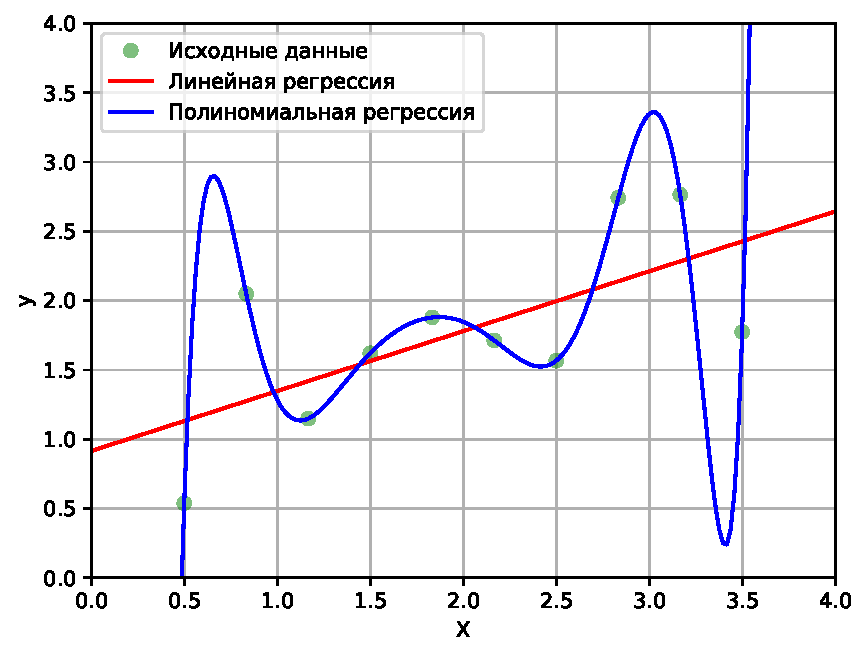
\includegraphics[width=0.5\textwidth]{overfitting_polynomial}
        \caption{Иллюстрация оверфитинга в случае полиномиальной модели.
                 Использовался полином десятой степени.}
        \label{pic:overfitting_polynomial}
    \end{figure}

    После идентификации для модели линейной регрессии получились следующие 
    параметры:
    \begin{description}
    	\item[a] -- коэффициент, характеризующий наклон, равен приблизительно 0.43;
    	\item[b] -- коэффициент, характеризующий смещение, равен приблизительно 0.92;
    	\item[RMSE] -- корень из среднеквадратической ошибки, равный приблизительно 0.48.
    \end{description}
    Как и ожидалось, полученные значения очень близки к параметрам выражения 
    \ref{eq:fake_results}.

    Не будем приводить все коэффициенты полиномиальной регрессии, корень из
    среднеквадратической ошибки для данной модели получился равным 
    $4.24 \cdot 10^{-11}$, на рисунке \ref{pic:overfitting_polynomial} видно, что
    график полиномиальной регрессии проходит через все точки исходных данных,
    при этом крайне маловероятно, что данная модель будет адекватно предсказывать
    значения $y(x)$, на значениях $x$, которых не было в тренировочном наборе.

    Для сравнения попробуем идентифицировать многоэкспоненциальную модель на 
    том же наборе данных, примем параметр n\_exps равным 10. Результаты 
    идентификации такой модели представлены на рисунке 
    \ref{pic:overfitting_multiexp}.

    \begin{figure}[!htp]
        \centering
        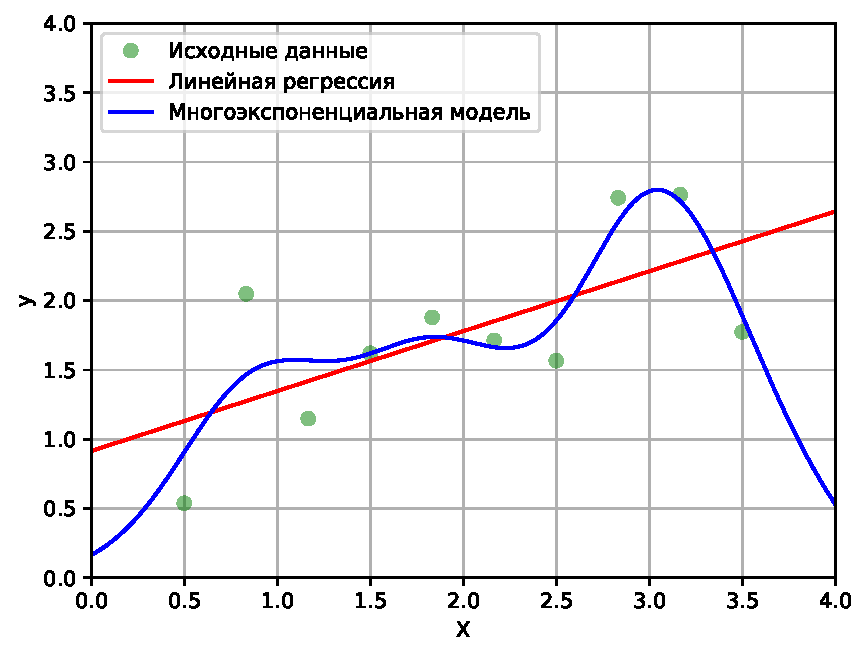
\includegraphics[width=0.5\textwidth]{overfitting_multiexp}
        \caption{Иллюстрация оверфитинга в случае многоэкспоненциальной модели.
                 Использовалась модель с параметром n\_exps = 10.}
        \label{pic:overfitting_multiexp}
    \end{figure}

    Для полученной многоэкспоненциальной модели с параметром n\_exps, равным 10
    корень из среднеквадратической ошибки получается приблизительно равным 0.28,
    что значительно больше, чем в случае полиномиальной регрессии, и всё еще 
    меньше, чем в случае линейной регрессии. При этом, хочется подчеркнуть, что
    данный набор точек является линейной функцией с добавлением нормально
    распределённой случайной составляющей (выражение \ref{eq:fake_results}).

    Существует несколько способов борьбы с оверфитингом, ниже приведены некоторые
    из них:
    \begin{itemize}
    	\item собрать больше данных (для того чтобы предыдущие примеры были 
    	показательны был намеренно сделан набор из 10 точек, получить аналогичный
    	эффект на наборе из 1000 точек сложнее);
    	\item 
    	\item использовать регуляризацию;
    	\item оценивать качество модели не на тренировочном наборе, а на отдельном
    	валидационном наборе (англ. validation set), случайно отобранной 
    	контрольной группе;
    	\item использовать приём, называемый кросвалидацией (англ. 
    	cross-validation) \cite{hands_on_ml}, \cite{sklearn_cross_validation}.
    \end{itemize}

    В задачах машинного обучения для того, чтобы оценить как точно модель 
    будет предсказывать целевые значения на новых данных, исходный набор 
    разделяют на даве группы: тренировочную и тестовою. На тренировачном наборе
    данных проводится идентификация модели, а на тестовом только оценивают 
    качество самой финальной модели. Таким образом, применительно к задаче 
    регрессии, ожидается, что на новых, невходивших в тренировочный набор данных
    модель будет демонстрировать среднеквадратическую ошибку, близкую к 
    полученной на тестовом наборе.

    Если у модели есть параметр, не зависящий от данных, например, степень
    алгебраического полинома или количество экспоненциальных составляющих 
    многоэкспоненциальной модели (параметр n\_exps), и необходимо найти 
    оптимальное значение данного параметра, то из тренировочного набора выделяют
    еще один набор данных -- валидационный набор, на котором оценивают
    оценивают модель при каждом значении подстраемового параметра, в итоге
    выбор останавливают на параметре с которым модель показала лучший результат
    (наименьшее значение среднеквадратической ошибки). При этом модель не 
    тренируют на валидационном наборе, то есть тренировочный набор уменьшается.

    Такой подход позволяет исключить оверфитинг и прогнозировать эффективность 
    модели. Однако, использование валидационного набора приводит к сокращению
    тренировочных данных, что может вызывать проблемы в случаях работы с 
    наборами данных, содержащих малое количество наблюдений. В таких случаях
    прибегают к технике, называемой кросвалидацией \cite{hands_on_ml}, 
    \cite{sklearn_cross_validation}.

    \begin{figure}[!htp]
        \centering
        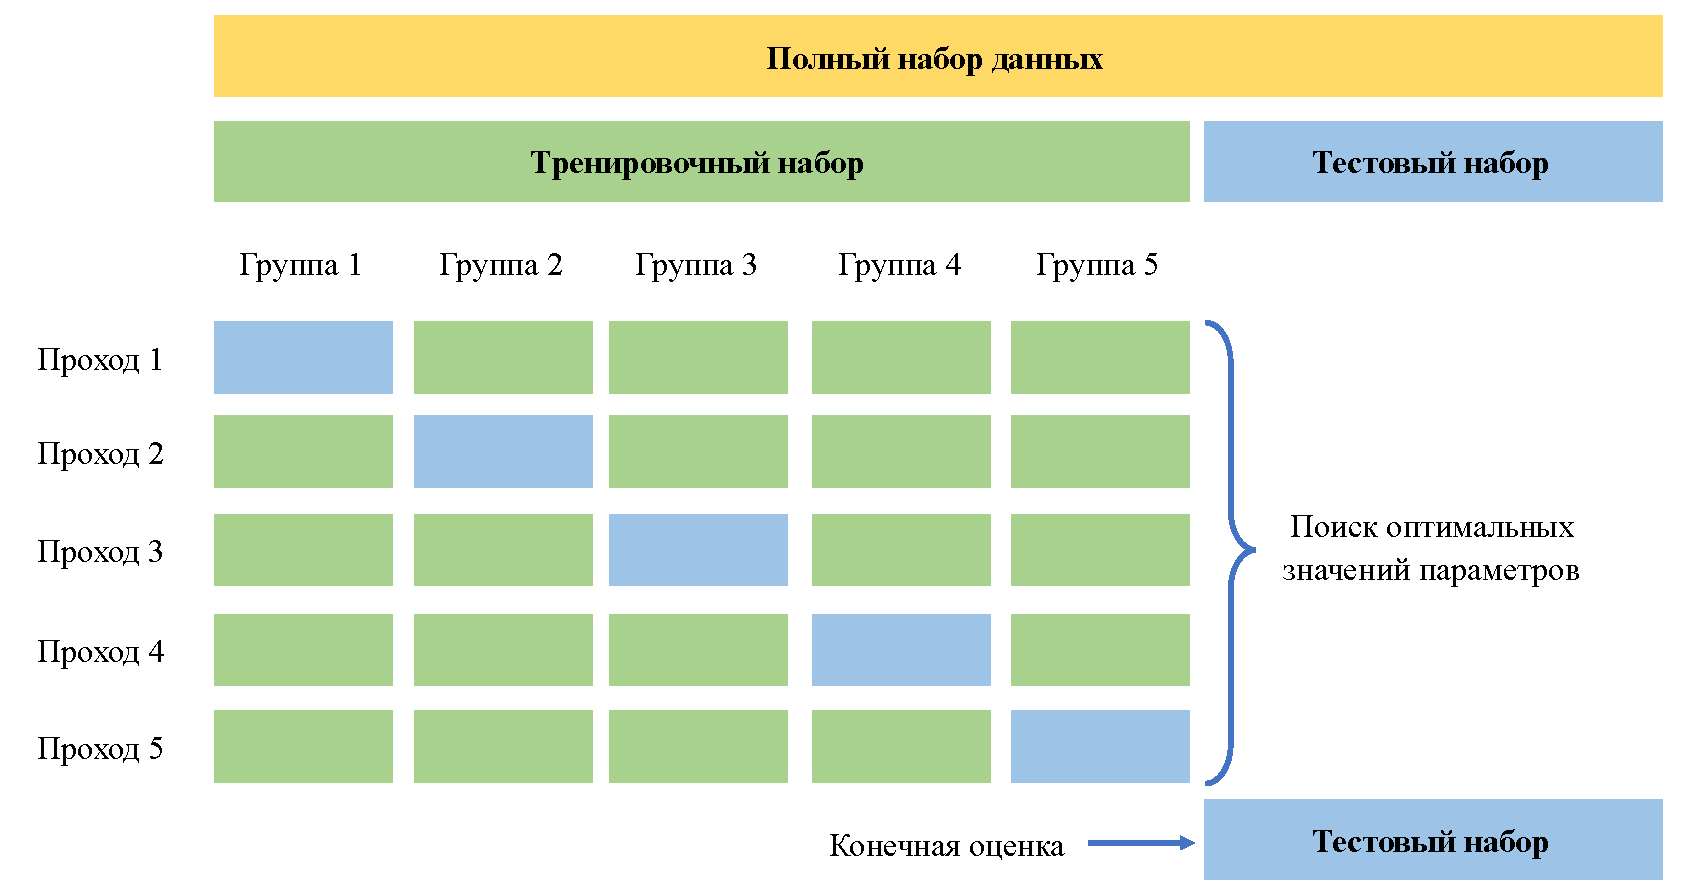
\includegraphics[width=0.75\textwidth]{cross_val}
        \caption{Иллюстрация кросвалидации.}
        \label{pic:cross_val}
    \end{figure}

    \section{Апробация моделей на экспериментальных данных}
	Для апробации разработанных моделей выберем результаты измерений на интергральной 
	схеме 1564ЛЕ1, состоящие из трёх частотных сканов, полученных при температурах 
	263~К, 283~К, 303~К. К сожалению, полученные частотные сканы содержат относительно 
	немного точек: 340, 340 и 34, соответственно. Поскольку требуется только 
	идентификация параметров модели, а не вычисление сигнала DLTS по новым значениям 
	частоты опорной функции, предлагается отказаться от оценки идентифицированной 
	модели на тестовом наборе, и ограничиться только оценками корня из 
	среднеквадратической ошибки (RMSE) на тренировочных данных и кросвалидацией.

	В данном разделе приводятся схема подключения образца, условия эксперимента,
	результаты измерений (частотные сканы), результаты идентификации частотных сканов
	разными моделями и их сравнение, а также анализ графиков Аррениуса, построенных 
	по вычисленным параметрам моделей.

	\subsection{Экспериментальные данные}
	\emph{Цель исследования}: регистрация частотных сканов интегральной схемы
	1564ЛЕ1 №1 в двухполюсном включении при разных температурах. Схема 
	подключения с эквивалентным диодом показана на рисунке~\ref{pic:scheme}. 

	\begin{figure}[!ht]
		\centering
		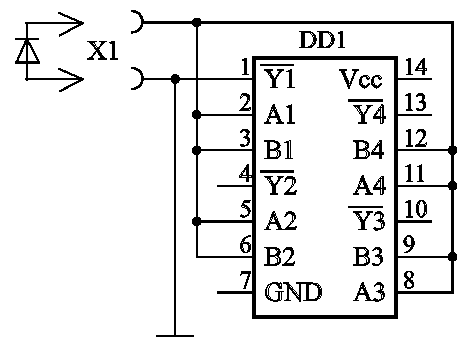
\includegraphics[width=0.4\textwidth]{scheme}
		\caption{Схема двухполюсного включения ИС 1564ЛЕ1.}
		\label{pic:scheme}
	\end{figure}

	Условия, одинаковые для всех сканов перечислены в таблице 
	\ref{table:common_conditions}. Графики с результатфми измерений 
	предствалены на рисунках \ref{pic:train_data_263}, \ref{pic:train_data_283}
	и \ref{pic:train_data_303}.

	\begin{table}[!ht]
		\centering
		\caption{Условия, одинаковые для всех сканов.}
		\begin{tabular}{|l|l|}
			\hline
			Параметр                           & Значение             \\ \hline
			Образцы                            & 1564ЛЕ1~№1           \\ \hline
			Длительность импульса              & 10                   \\ 
			заполнения, мкс                    &                      \\ \hline
			$U_1$                              & -4 В                 \\ \hline
			$U_r$                              & -5 В                 \\ \hline
			Автоматическая компенсация моста   & включена             \\ \hline
			Начальная частота сканирования, Гц & 1                    \\ \hline
			Конечная  частота сканирования, Гц & 2500                 \\ \hline
			Направление сканирования           & вниз по частоте      \\ \hline
			Интервал между измерениями, с      & 3.5                  \\ \hline
			Постоянная интегрирования, с       & 3                    \\ \hline
		\end{tabular}
		\label{table:common_conditions}
	\end{table}

	\begin{figure}[!htp]
		\centering
		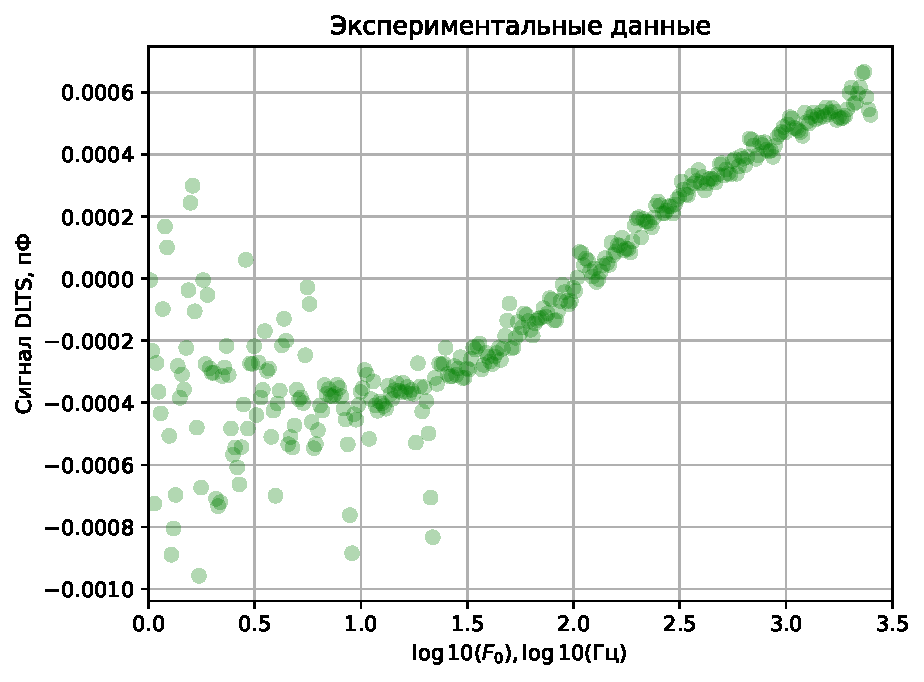
\includegraphics[width=0.5\textwidth]{1564ЛЕ1№1_п1_2500Гц-1Гц_1пФ_-10С_-4В-5В_10мВ_10мкс_шаг_0,01_train_data}
		\caption{Частотный скан, полученный при температуре 263 К.}
		\label{pic:train_data_263}
	\end{figure}

	\begin{figure}[!htp]
		\centering
		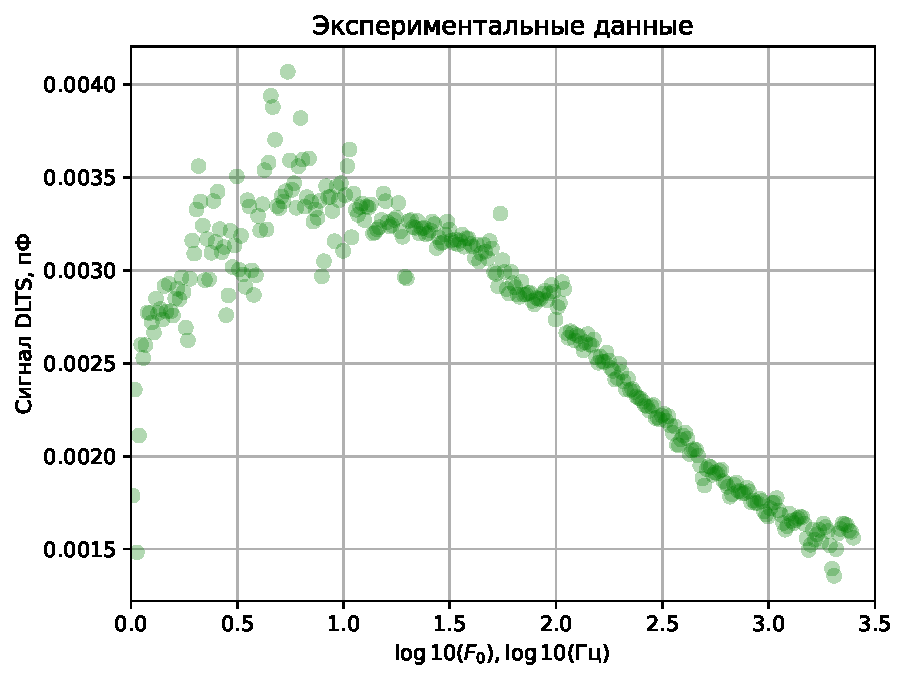
\includegraphics[width=0.5\textwidth]{1564ЛЕ1№1_п1_2500Гц-1Гц_1пФ_+10С_-4В-5В_50мВ_10мкс_шаг_0,01_train_data}
		\caption{Частотный скан, полученный при температуре 283 К.}
		\label{pic:train_data_283}
	\end{figure}

	\begin{figure}[!htp]
		\centering
		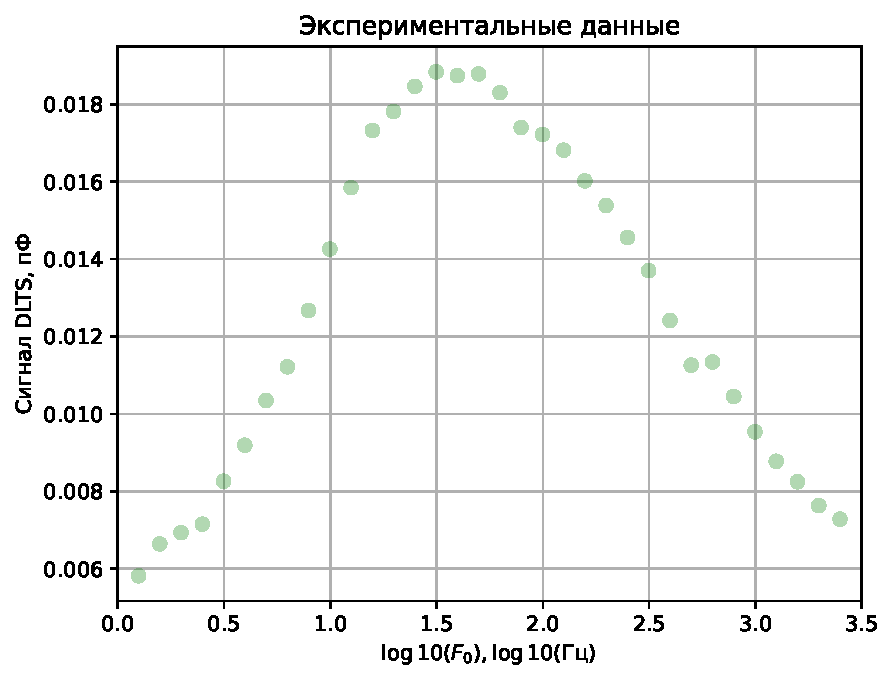
\includegraphics[width=0.5\textwidth]{1564ЛЕ1№1_п1_2500Гц-1Гц_10пФ_+30С_-4В-5В_50мВ_10мкс_шаг_0,1_train_data}
		\caption{Частотный скан, полученный при температуре 303 К.}
		\label{pic:train_data_303}
	\end{figure}


	\newpage
	\subsection{Частотный скан при температуре 263 К}
	\subsubsection{Моноэкспоненциальная модель с показателем $p$}

	Как показано на рисунке \ref{pic:train_data_263}, частотный скан имеет два
	пика: положительный и отрицательный, поэтому сначала выполним идентификацию
	модели с показателем $p$ с начальными параметрами близкими к положительному
	пику. Результат идентификации представлен на рисунке 
	\ref{pic:model_monoexp_p_positive_263}.

	\begin{figure}[!htp]
		\centering
		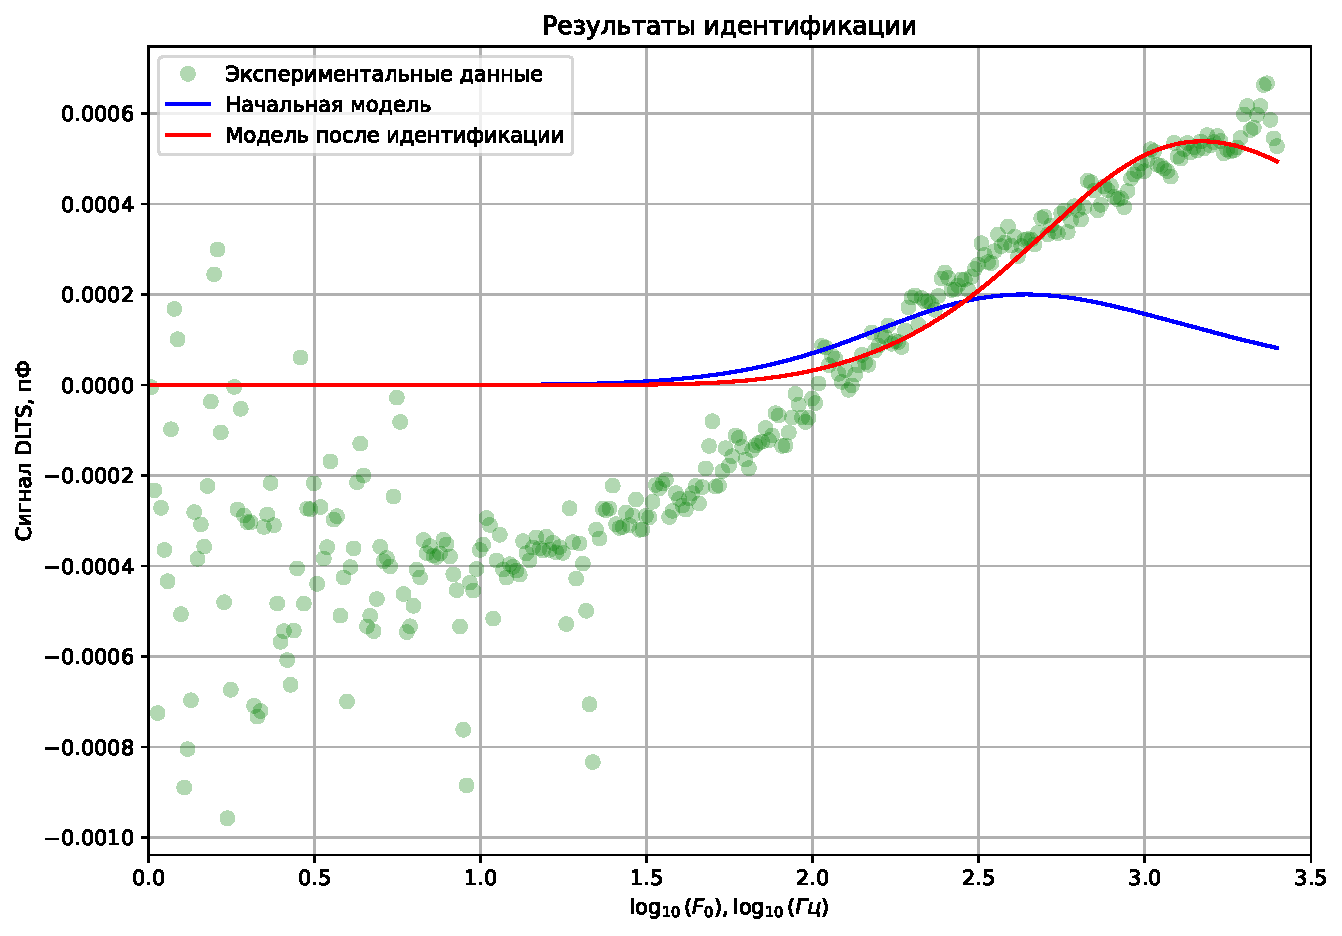
\includegraphics[width=0.75\textwidth]{1564ЛЕ1№1_п1_2500Гц-1Гц_1пФ_-10С_-4В-5В_10мВ_10мкс_шаг_0,01_single_exp_model_1}
		\caption{Результат идентификации положительного пика частотного скана
		         при $T=263K$.}
		\label{pic:model_monoexp_p_positive_263}
	\end{figure}

	Для того, чтобы убедиться, что алгоритм идентификации достиг минимума 
	функции потерь, построим график значений среднеквадратической ошибки на 
	каждой итерации, график нормируем оносительно максимального значения метрики.
	Получившийся график представлен на рисунке \ref{pic:loss_monoexp_p_positive_263}.

	\begin{figure}[!htp]
		\centering
		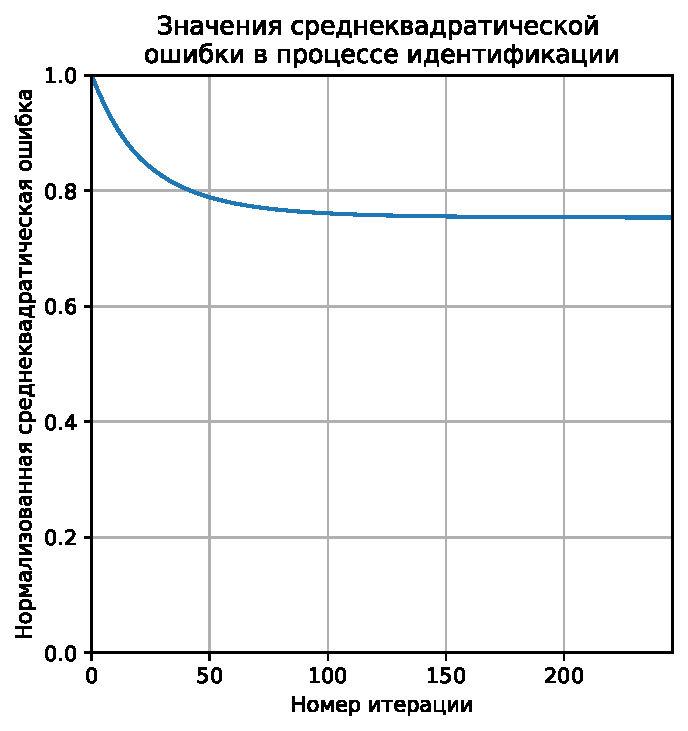
\includegraphics[width=0.35\textwidth]{1564ЛЕ1№1_п1_2500Гц-1Гц_1пФ_-10С_-4В-5В_10мВ_10мкс_шаг_0,01_single_exp_model_loss_1}
		\caption{График среднеквадратической ошибки в процессе идентификации,
		         нормированной относительно её максимального значения.}
		\label{pic:loss_monoexp_p_positive_263}
	\end{figure}

	График среднеквадратической ошибки выходит на <<плато>>, что свидетельствует 
	о том, что решение сошлось, однако довольно высокое значение 
	среднеквадратической ошибки может указывать на то, что алгоритм нашёл 
	локальный минимум функции потерь.

	Построим график отклонений результатов моделирования от экспериментальных 
	данных (рисунок \ref{pic:deviations_monoexp_p_positive_263}), чтобы оценить 
	систематическую ошибку.

	\begin{figure}[!htp]
		\centering
		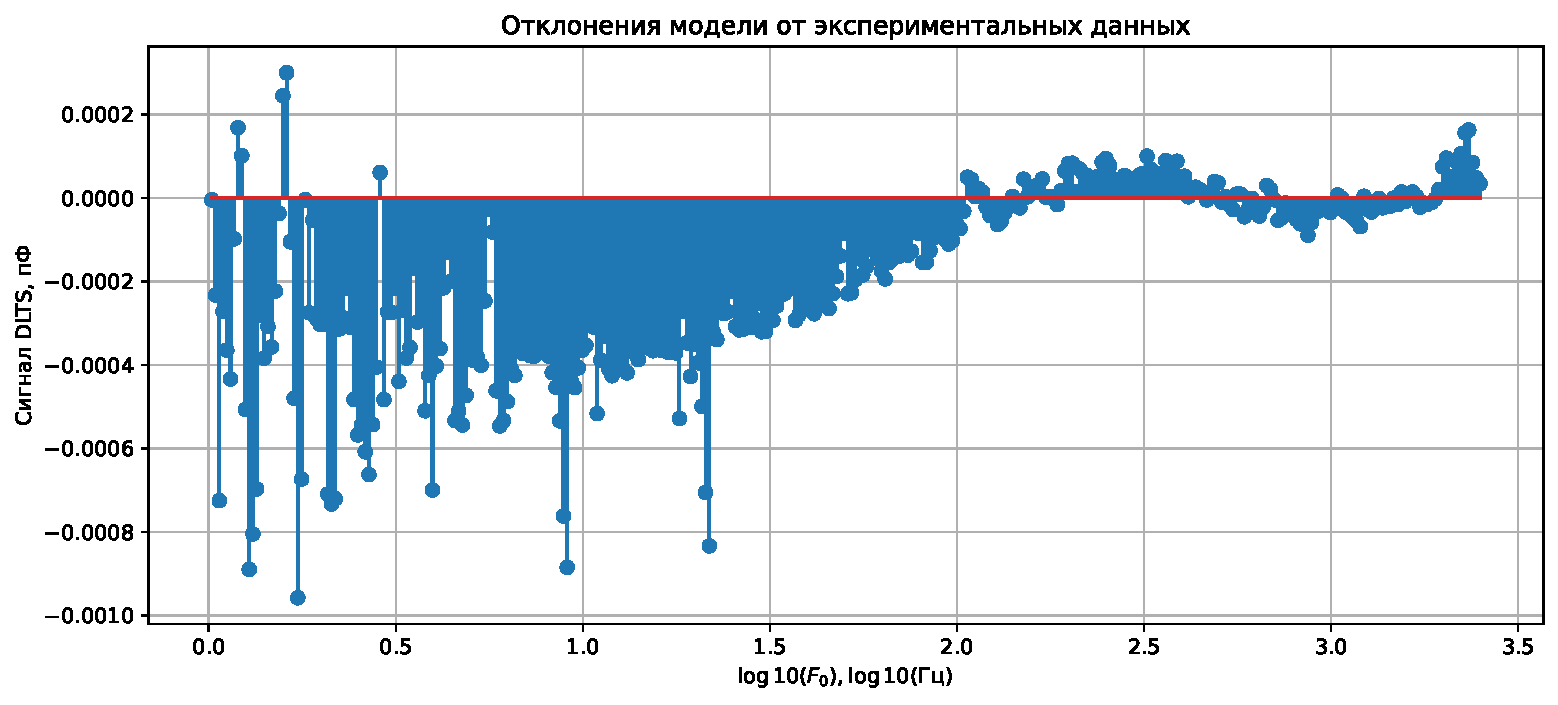
\includegraphics[width=0.75\textwidth]{1564ЛЕ1№1_п1_2500Гц-1Гц_1пФ_-10С_-4В-5В_10мВ_10мкс_шаг_0,01_single_exp_deviations_1}
		\caption{График отклонений результатов, полученных на идентифицированной
		модели, от экспериментальных данных.}
		\label{pic:deviations_monoexp_p_positive_263}
	\end{figure}

	Рисунки \ref{pic:model_monoexp_p_positive_263} и 
	\ref{pic:deviations_monoexp_p_positive_263} демонстрируют, что модель не 
	охватывает половину частотного скана с отрицательными значениями сигнала
	DLTS, что закономерно для однопиковой модели.

	Построим гистограму распределения отклонений резульатов моделирования от
	экспериментальных данных. В идеальном случае данное распределение должно
	стремиться к распределению погрешностей измерительного прибора и быть близко
	к нормальному распределению, в данном случае (рисунок 
	\ref{pic:hist_monoexp_p_positive_263}) это не так. На рисунке 
	\ref{pic:hist_monoexp_p_positive_263} сплошной линией показан результат
	сглаживания гистограммы c гаусовым усредняющим ядром (в англоязычной 
	литературе данный алгоритм называется <<kernel density estimation>>).

	\begin{figure}[!htp]
		\centering
		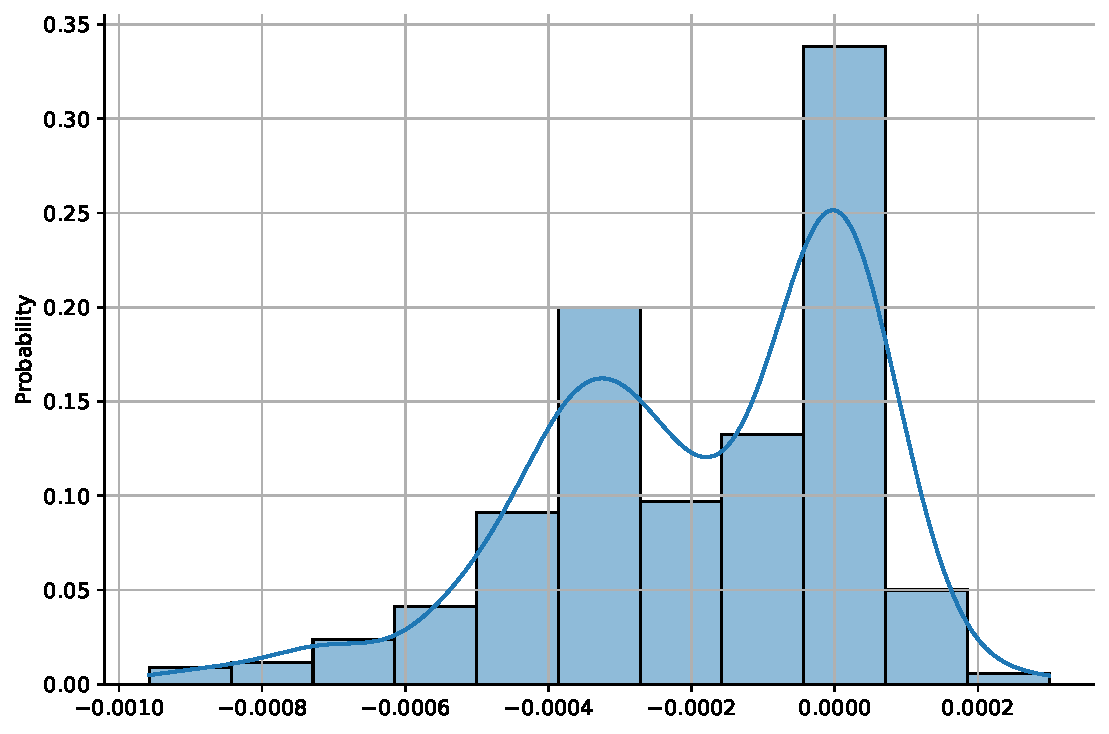
\includegraphics[width=0.5\textwidth]{1564ЛЕ1№1_п1_2500Гц-1Гц_1пФ_-10С_-4В-5В_10мВ_10мкс_шаг_0,01_single_exp_hist_1}
		\caption{Гистограмма отклонений данных, полученных на идентифицированной 
		         модели, от экспериментальных данных. Сплошной линией показан 
		         результат сглаживания гистограммы.}
		\label{pic:hist_monoexp_p_positive_263}
	\end{figure}

	В таблице \ref{table:results_monoexp_p_positive_263} приведём параметры 
	идентифицированной модели и результаты оценок точности моделирования.

	\begin{table}[!htp]
    	\centering
    	\caption{Результаты идентификации модели}
		\begin{tabular}{|l|l|}
			\hline
			Параметр                           & Значение  \\ \hline
			Постоянна времени $\tau$, с        & 0,000286  \\ \hline
			Амплитуда, пФ                      & 0.000538  \\ \hline
			Показатель $p$                     & 0.802     \\ \hline
			Результат кросвалидации (RMSE), пФ & 0.000290  \\ \hline
			RMSE, пФ                           & 0.000291  \\ \hline
		\end{tabular}
		\label{table:results_monoexp_p_positive_263}
	\end{table}

	Построим полученный спектр частотного скана (рисунок 
	\ref{pic:spectr_monoexp_p_positive_263}), чтобы предствить
	результаты в более наглядной форме.

	\begin{figure}[!htp]
		\centering
		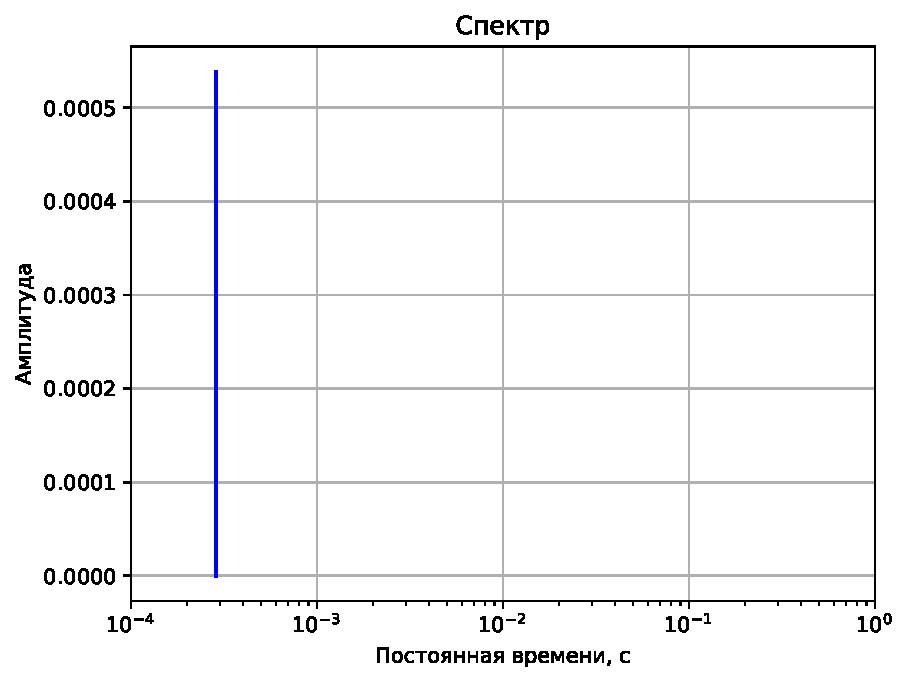
\includegraphics[width=0.5\textwidth]{1564ЛЕ1№1_п1_2500Гц-1Гц_1пФ_-10С_-4В-5В_10мВ_10мкс_шаг_0,01_single_exp_spectr_1}
		\caption{Спектр сигнала релаксации ёмкости. Амплитуда указана в пФ.}
		\label{pic:spectr_monoexp_p_positive_263}
	\end{figure}

	Идентифицируем эту же модель с начальными параметрами близкими к параметрам
	отрицательного пика. На рисунке \ref{pic:model_monoexp_p_negative_263}
	представлен график с результатами идентификации.

	\begin{figure}[!htp]
		\centering
		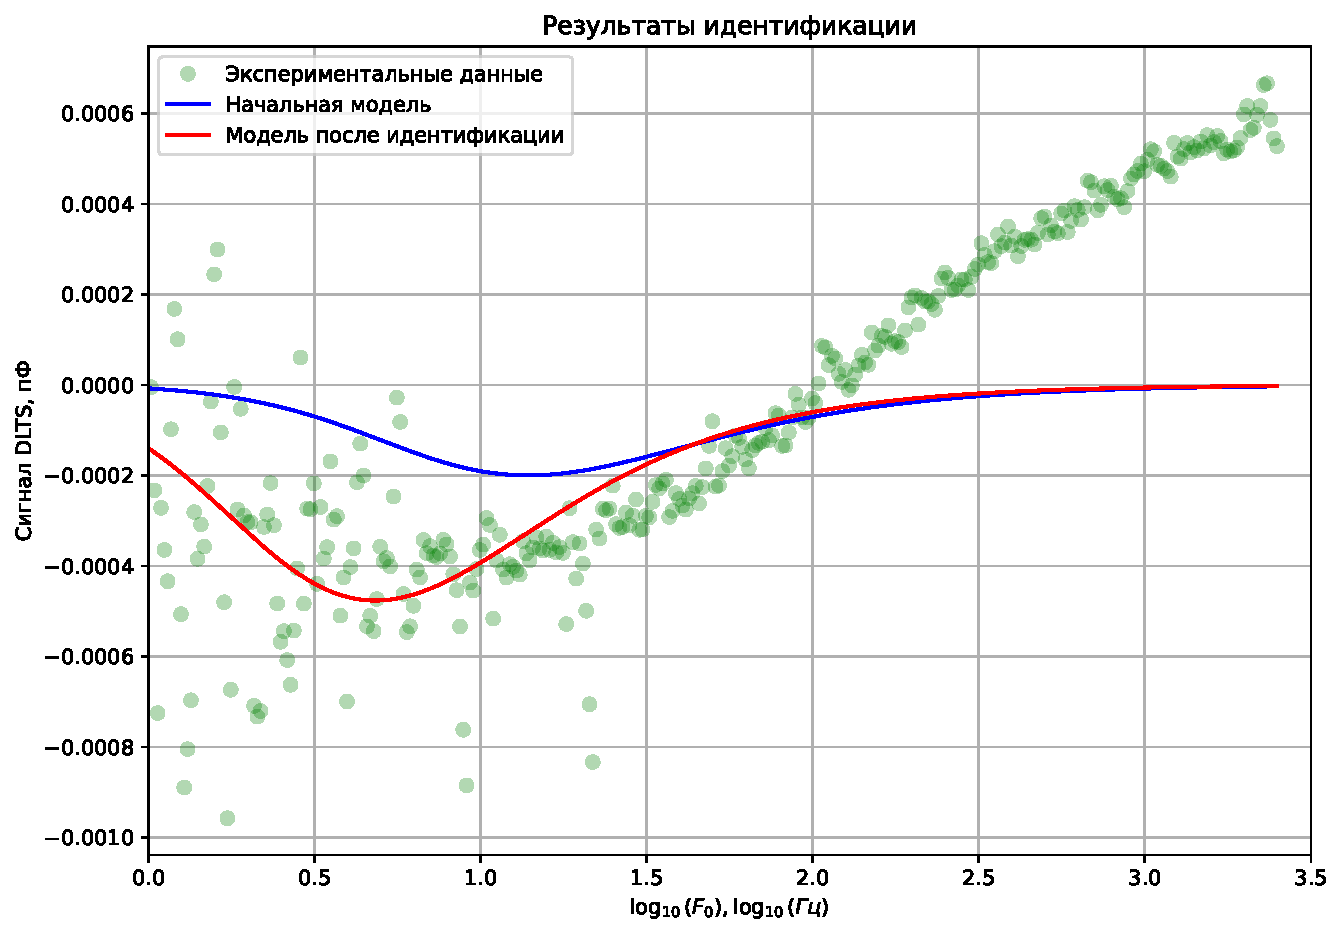
\includegraphics[width=0.75\textwidth]{1564ЛЕ1№1_п1_2500Гц-1Гц_1пФ_-10С_-4В-5В_10мВ_10мкс_шаг_0,01_single_exp_model_2}
		\caption{Результат идентификации отрицательного пика частотного скана
		         при $T=263K$.}
		\label{pic:model_monoexp_p_negative_263}
	\end{figure}

	На рисунке \ref{pic:loss_monoexp_p_negative_263} представлен график значений
	нормированной среднеквадратической ошибки на каждой итерации. На итерациях
	с номерами выше 200 значения среднеквадратической ошибки практически не 
	изменяются, очевидно, алгоритм нашёл минимум.

	\begin{figure}[!htp]
		\centering
		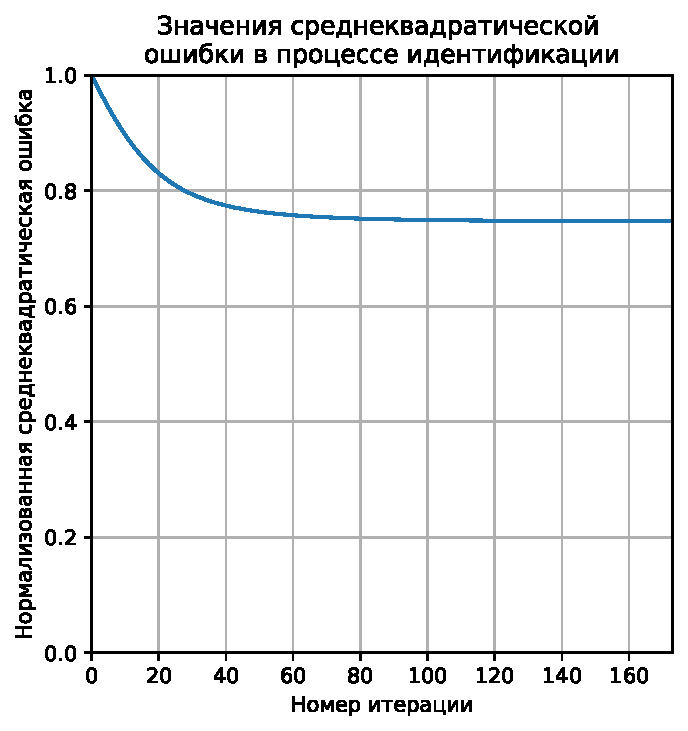
\includegraphics[width=0.35\textwidth]{1564ЛЕ1№1_п1_2500Гц-1Гц_1пФ_-10С_-4В-5В_10мВ_10мкс_шаг_0,01_single_exp_model_loss_2}
		\caption{График среднеквадратической ошибки в процессе идентификации,
		         нормированной относительно её максимального значения.}
		\label{pic:loss_monoexp_p_negative_263}
	\end{figure}

	На гафике отклонений результатов моделирования от экспериментальных данных
	(рисунок \ref{pic:deviations_monoexp_p_negative_263}) видно, что теперь 
	модель <<не охватывает>> диапазон высоких частот опорной функции, где
	располагается положительный пик.

	\begin{figure}[!htp]
		\centering
		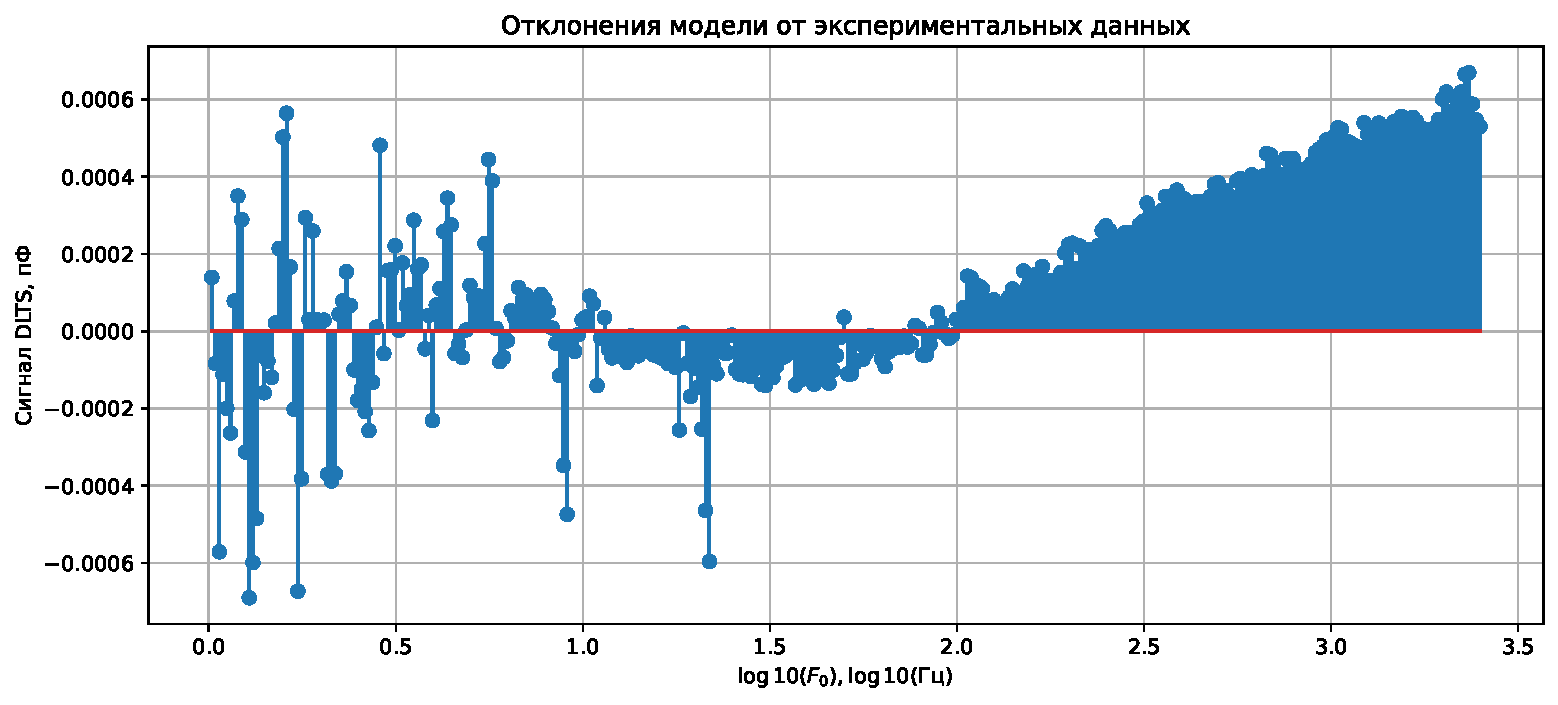
\includegraphics[width=0.75\textwidth]{1564ЛЕ1№1_п1_2500Гц-1Гц_1пФ_-10С_-4В-5В_10мВ_10мкс_шаг_0,01_single_exp_deviations_2}
		\caption{График отклонений результатов, полученных на идентифицированной
		модели, от экспериментальных данных.}
		\label{pic:deviations_monoexp_p_negative_263}
	\end{figure}

	Гистограмма отклонений (рисунок \ref{pic:hist_monoexp_p_negative_263}) 
	далека от нормального распределения. Сплошной линией показан результат 
	сглаживания гистограммы.

	\begin{figure}[!htp]
		\centering
		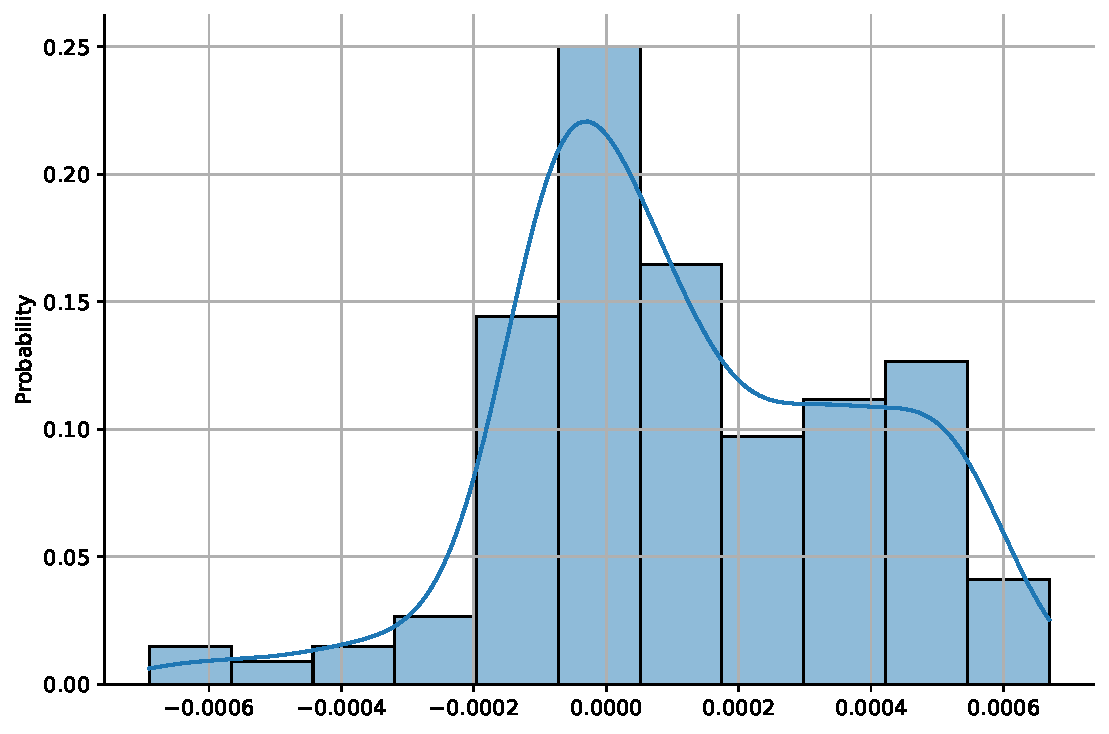
\includegraphics[width=0.5\textwidth]{1564ЛЕ1№1_п1_2500Гц-1Гц_1пФ_-10С_-4В-5В_10мВ_10мкс_шаг_0,01_single_exp_hist_2}
		\caption{Гистограмма отклонений данных, полученных на идентифицированной 
		         модели, от экспериментальных данных. Сплошной линией показан 
		         результат сглаживания гистограммы.}
		\label{pic:hist_monoexp_p_negative_263}
	\end{figure}

	В таблице \ref{table:results_monoexp_p_negative_263} приведём параметры 
	идентифицированной модели и результаты оценок точности моделирования.

	\begin{table}[!htp]
    	\centering
    	\caption{Результаты идентификации модели}
		\begin{tabular}{|l|l|}
			\hline
			Параметр                           & Значение   \\ \hline
			Постоянна времени $\tau$, с        &  0.091434  \\ \hline
			Амплитуда, пФ                      & -0.000476	\\ \hline
			Показатель $p$                     &  1.036     \\ \hline
			Результат кросвалидации (RMSE), пФ &  0.000287  \\ \hline
			RMSE, пФ                           &  0.000286  \\ \hline
		\end{tabular}
		\label{table:results_monoexp_p_negative_263}
	\end{table}

	Построим полученный спектр частотного скана (рисунок 
	\ref{pic:spectr_monoexp_p_negative_263}), чтобы представить результаты в 
	более наглядной форме.

	\begin{figure}[!htp]
		\centering
		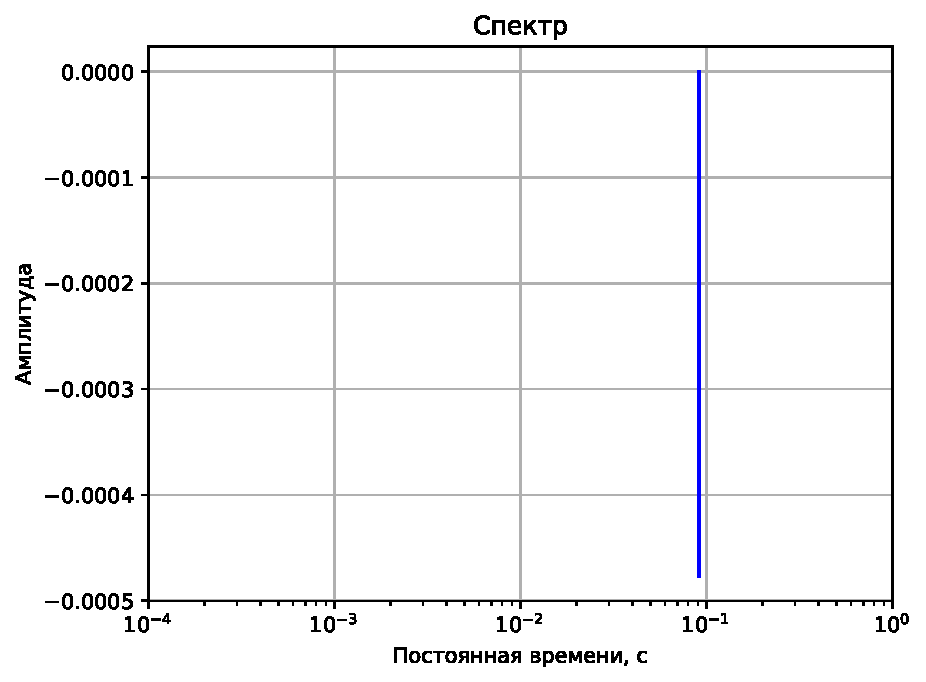
\includegraphics[width=0.5\textwidth]{1564ЛЕ1№1_п1_2500Гц-1Гц_1пФ_-10С_-4В-5В_10мВ_10мкс_шаг_0,01_single_exp_spectr_2}
		\caption{Спектр сигнала релаксации ёмкости.}
		\label{pic:spectr_monoexp_p_negative_263}
	\end{figure}

	
	\newpage
	\subsubsection{Моноэкспоненциальная модель с показателем $p=1$}
	Для сравнения, на тех же данных выполним идентификацию модели идеального 
	частотного скана. В этот раз инициализацию модели выполним случайными 
	значениями. Результаты идентификации представлены на рисунке 
	\ref{pic:model_single_exp_ideal_263}.

	\begin{figure}[!htp]
		\centering
		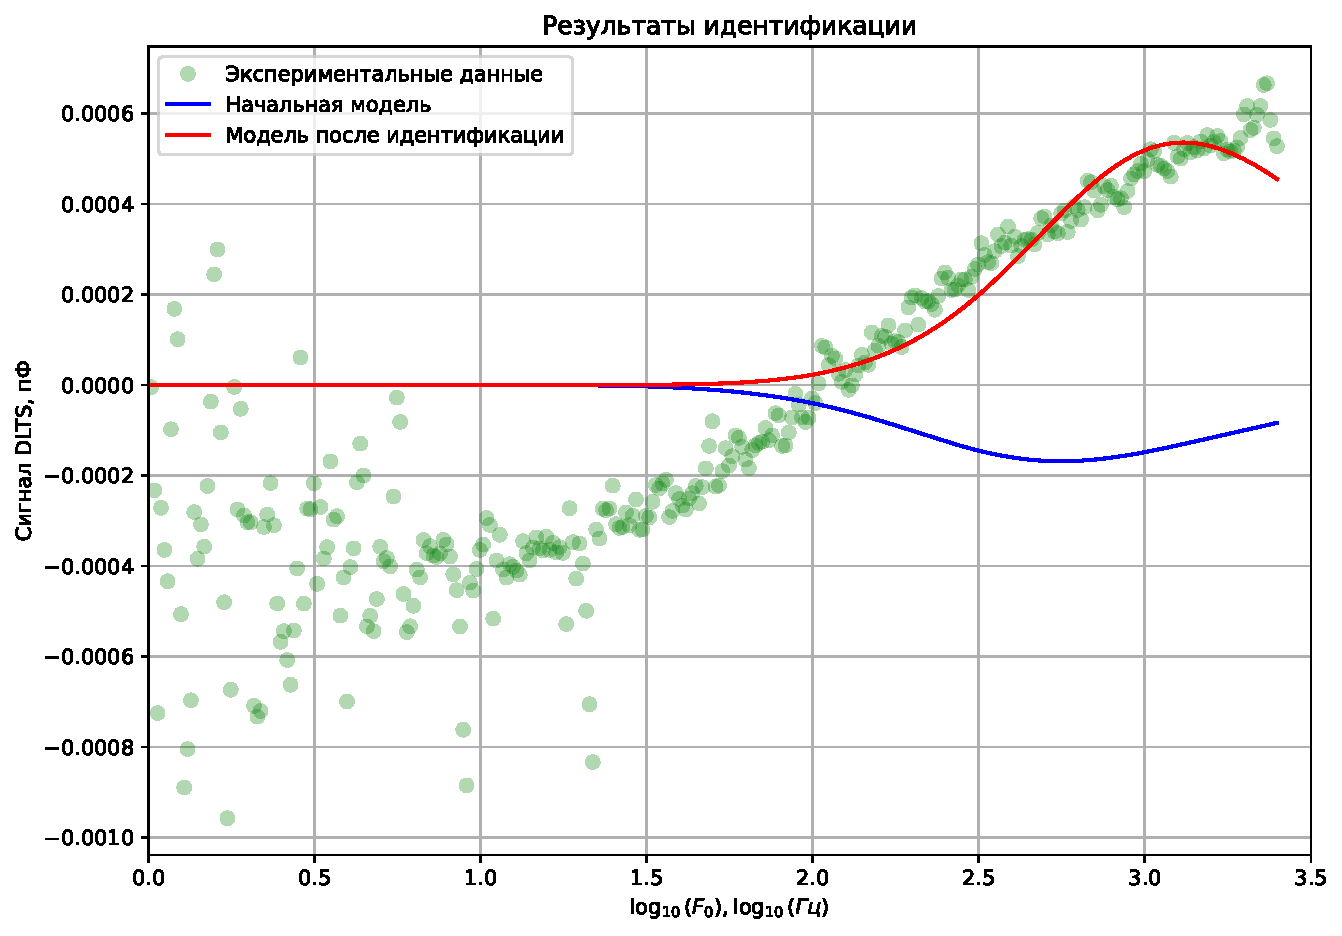
\includegraphics[width=0.75\textwidth]{1564ЛЕ1№1_п1_2500Гц-1Гц_1пФ_-10С_-4В-5В_10мВ_10мкс_шаг_0,01_single_exp_ideal_model}
		\caption{Результат идентификации модели частотного скана при $T=263K$.}
		\label{pic:model_single_exp_ideal_263}
	\end{figure}

	В данном случае алгоритм идентификации нашёл локальный минимум, 
	соответствующий положительному пику. Полученные результаты качественно похожи
	на результаты идентификации из предыдущего раздела. На рисунках 
	\ref{pic:loss_single_exp_ideal_263}, \ref{pic:deviations_single_exp_ideal_263},
	\ref{pic:hist_single_exp_ideal_263} показаны график значений 
	среднеквадратической ошибки на каждой итерации, график отклонений результатов
	моделирования от экспериментальных данных и гистограмма отклонений соответственно.

	\begin{figure}[!htp]
		\centering
		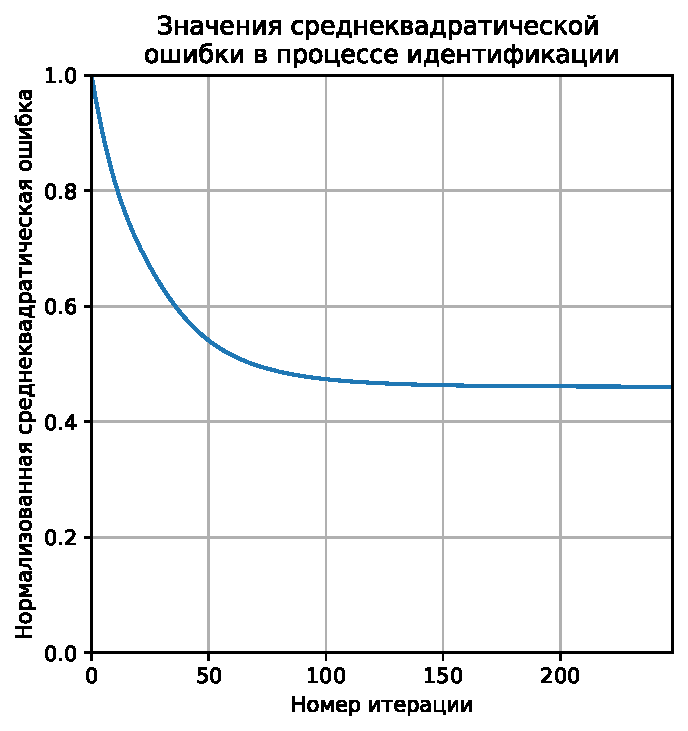
\includegraphics[width=0.35\textwidth]{1564ЛЕ1№1_п1_2500Гц-1Гц_1пФ_-10С_-4В-5В_10мВ_10мкс_шаг_0,01_single_exp_ideal_model_loss}
		\caption{График среднеквадратической ошибки в процессе идентификации,
		         нормированной относительно её максимального значения.}
		\label{pic:loss_single_exp_ideal_263}
	\end{figure}

	\begin{figure}[!htp]
		\centering
		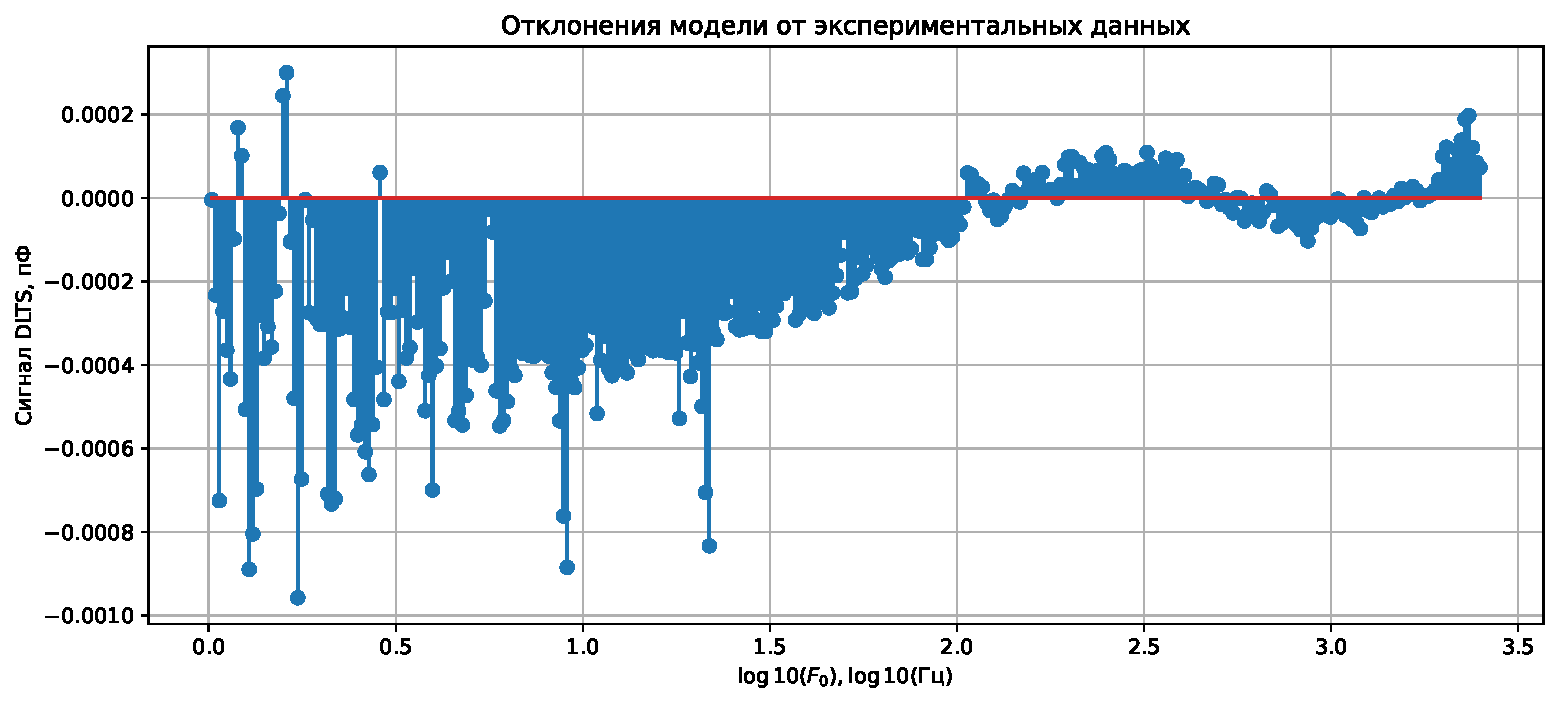
\includegraphics[width=0.75\textwidth]{1564ЛЕ1№1_п1_2500Гц-1Гц_1пФ_-10С_-4В-5В_10мВ_10мкс_шаг_0,01_single_exp_ideal_deviations}
		\caption{График отклонений результатов, полученных на идентифицированной
		модели, от экспериментальных данных.}
		\label{pic:deviations_single_exp_ideal_263}
	\end{figure}

	\begin{figure}[!htp]
		\centering
		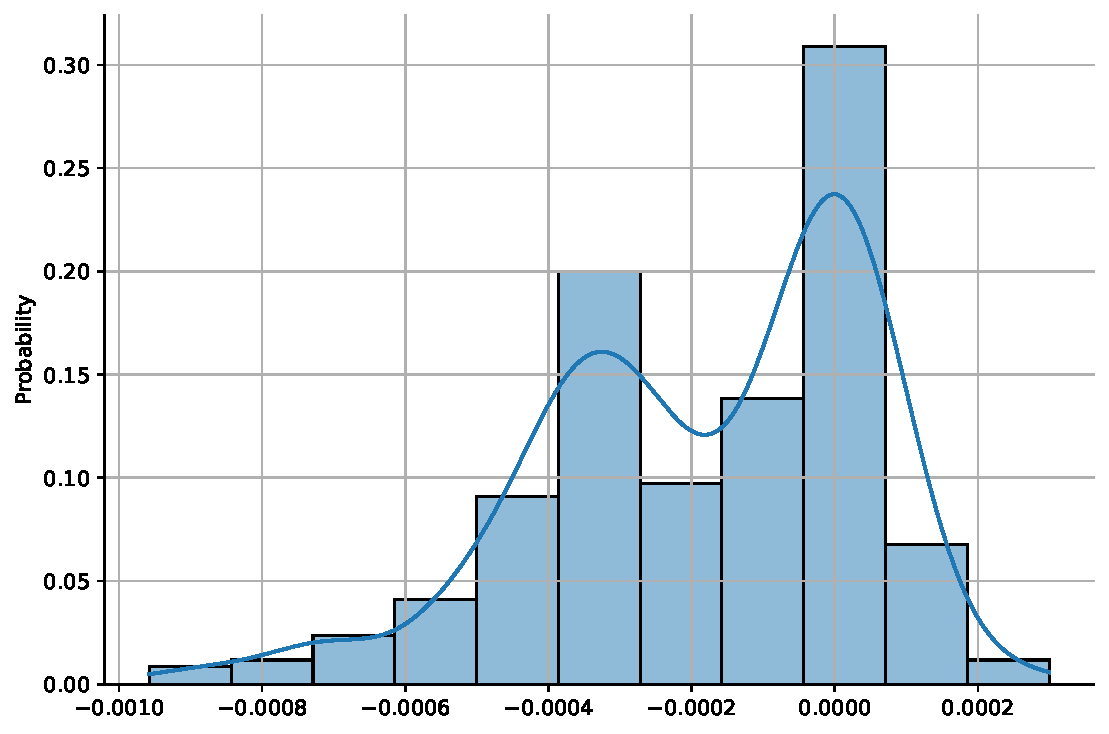
\includegraphics[width=0.5\textwidth]{1564ЛЕ1№1_п1_2500Гц-1Гц_1пФ_-10С_-4В-5В_10мВ_10мкс_шаг_0,01_single_exp_ideal_hist}
		\caption{Гистограмма отклонений данных, полученных на идентифицированной 
		         модели, от экспериментальных данных. Сплошной линией показан 
		         результат сглаживания гистограммы.}
		\label{pic:hist_single_exp_ideal_263}
	\end{figure}

	В таблице \ref{table:results_single_exp_ideal_263} приведены параметры 
	идентифицированной модели и результаты оценок точности моделирования.

	\begin{table}[!htp]
    	\centering
    	\caption{Результаты идентификации модели}
		\begin{tabular}{|l|l|}
			\hline
			Параметр                           & Значение \\ \hline
			Постоянна времени $\tau$, с        & 0.000327 \\ \hline
			Амплитуда, пФ                      & 0.000536 \\ \hline
			Показатель $p$                     & 1.0      \\ \hline
			Результат кросвалидации (RMSE), пФ & 0.000279 \\ \hline
			RMSE, пФ                           & 0.000291 \\ \hline
		\end{tabular}
		\label{table:results_single_exp_ideal_263}
	\end{table}

	На рисунке \ref{pic:spectr_single_exp_ideal_263} приведён полученный спектр 
	частотного скана.

	\begin{figure}[!htp]
		\centering
		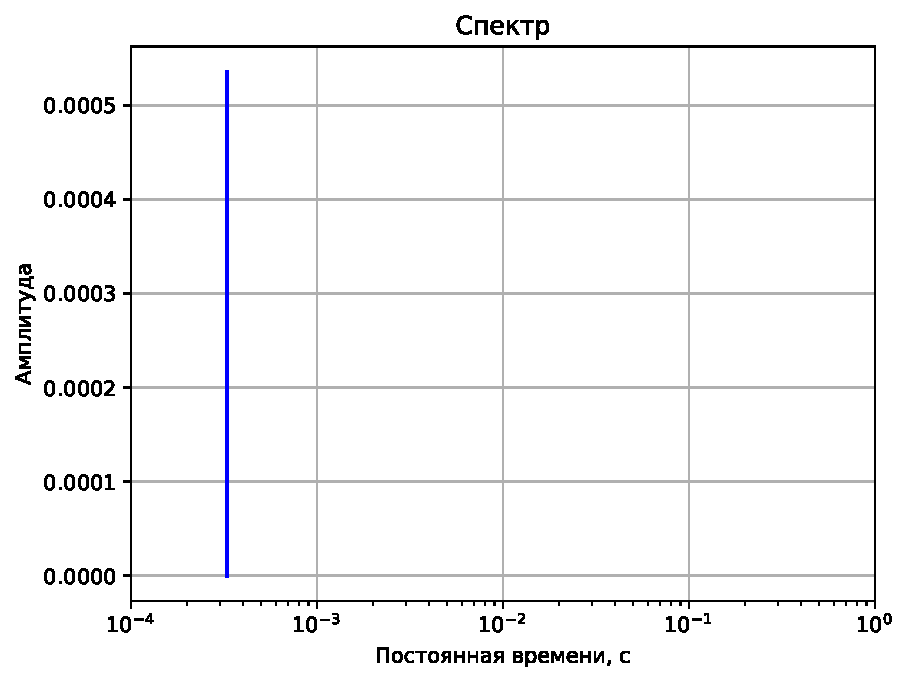
\includegraphics[width=0.5\textwidth]{1564ЛЕ1№1_п1_2500Гц-1Гц_1пФ_-10С_-4В-5В_10мВ_10мкс_шаг_0,01_single_exp_ideal_spectr}
		\caption{Спектр сигнала релаксации ёмкости.}
		\label{pic:spectr_single_exp_ideal_263}
	\end{figure}


	\newpage
	\subsubsection{Многоэкспоненциальная модель с n\_exps > 1}

	Выполним идентификацию многоэкспоненциальной модели. Особенность данной модели
	в том, что у неё есть параметр, независящий от данных -- количество
	экспоененциальных составляющих. По скольку у нас нет гипотезы о количестве
	экспоненциальных составляющих в релаксационном сигнале, воспользуемся приёмом,
	описанном в разделе \ref{section:quality_and_optimization}: для моделей
	с значениями параметра n\_exps равными 5, 6, 7, 8, 9 и 10 будем выполнять
	кросвалидацию, выберем ту, которая покажет лучший результат. В таблице
	\ref{table:multi_exp_model_263_cross_val} предсталены полученные результаты.
	Лучшей оказалась модель с параметром n\_exps = 8, то есть имеющая 8 
	экспоненциальных составляющих.

	\begin{table}[!htp]
    	\centering
    	\caption{Результаты кросвалидации для разных значений параметра n\_exps}
		\begin{tabular}{|l|l|}
		\hline
		Значение параметра n\_exps & Результат кросвалидации \\ \hline
		5                          & 0.0001373               \\ \hline
		6                          & 0.0001361               \\ \hline
		7                          & 0.0001347               \\ \hline
		8                          & 0.0001345               \\ \hline
		9                          & 0.0001353               \\ \hline
		10                         & 0.0001349               \\ \hline
		\end{tabular}
		\label{table:multi_exp_model_263_cross_val}
	\end{table}

	Результаты идентификации модели с восемью экспоненциальными составляющими
	предствалены на рисунке \ref{pic:multi_exp_model_263}. В данном случае,
	модель воспроизводит как положительный так и отрицательный пик.

	\begin{figure}[!htp]
		\centering
		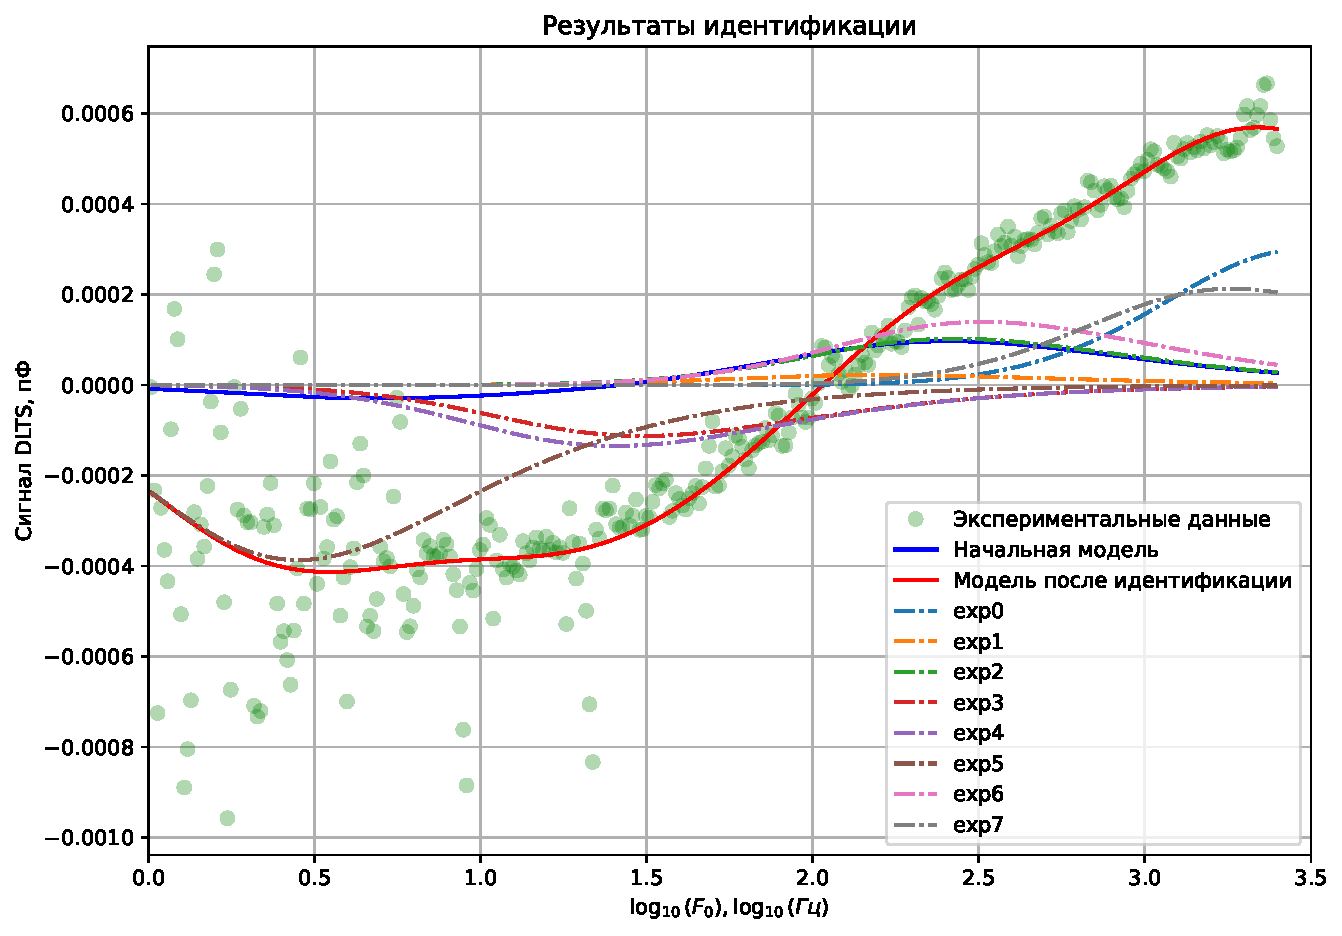
\includegraphics[width=0.75\textwidth]{1564ЛЕ1№1_п1_2500Гц-1Гц_1пФ_-10С_-4В-5В_10мВ_10мкс_шаг_0,01_multi_exp_model}
		\caption{Результат идентификации многоэкспоненциальной моделью 
		         частотного скана при $T=263K$.}
		\label{pic:multi_exp_model_263}
	\end{figure}

	По графику нормированной среднеквадратической ошибки, показанном на рисунке
	\ref{pic:multi_exp_loss_263}, видно, что алгоритм идентификации остановился
	из-за достижения максимального количества итераций. При этом, форма графика
	позволяет предположить, что полученные параметры модели близки к оптимальным.

	\begin{figure}[!htp]
		\centering
		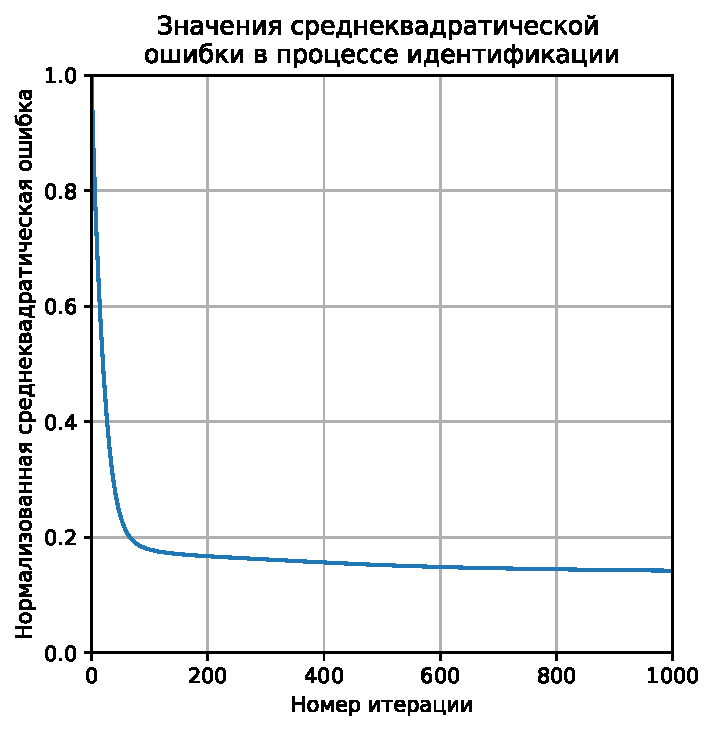
\includegraphics[width=0.35\textwidth]{1564ЛЕ1№1_п1_2500Гц-1Гц_1пФ_-10С_-4В-5В_10мВ_10мкс_шаг_0,01_multi_exp_loss}
		\caption{График среднеквадратической ошибки в процессе идентификации,
		         нормированной относительно её максимального значения.}
		\label{pic:multi_exp_loss_263}
	\end{figure}

	На рисунке \ref{pic:multi_exp_deviations_263} показан график отклонений
	результатов моделирования от экспериментальных данных. В отличие от двух
	предыдущих моделей, многоэкспоненциальная модель хорошо воспроизводит 
	как положительный, так и отрицательный пик. Увеличение разброса в области
	низких частот опорной функции связано с особенностями работы аппаратного
	интегратора спектрометра.

	\begin{figure}[!htp]
		\centering
		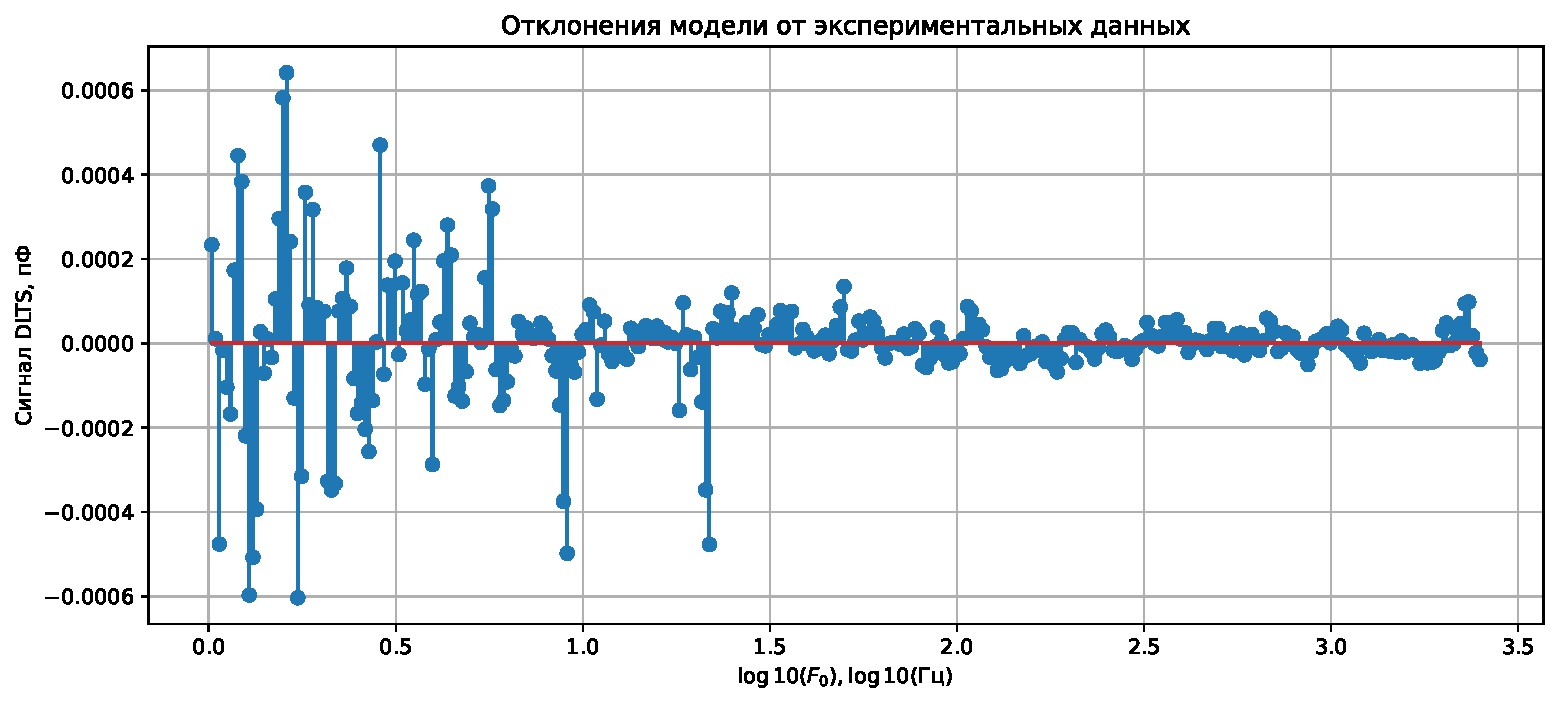
\includegraphics[width=0.75\textwidth]{1564ЛЕ1№1_п1_2500Гц-1Гц_1пФ_-10С_-4В-5В_10мВ_10мкс_шаг_0,01_multi_exp_deviations}
		\caption{График отклонений результатов, полученных на идентифицированной
		модели, от экспериментальных данных.}
		\label{pic:multi_exp_deviations_263}
	\end{figure}

	На рисунке \ref{pic:multi_exp_hist_263} показана гистограмма отклонений 
	данных, полученных на идентифицированной модели, от результатов измерений.
	Форма полученного распределения приближается к форме нормального распределения.

	\begin{figure}[!htp]
		\centering
		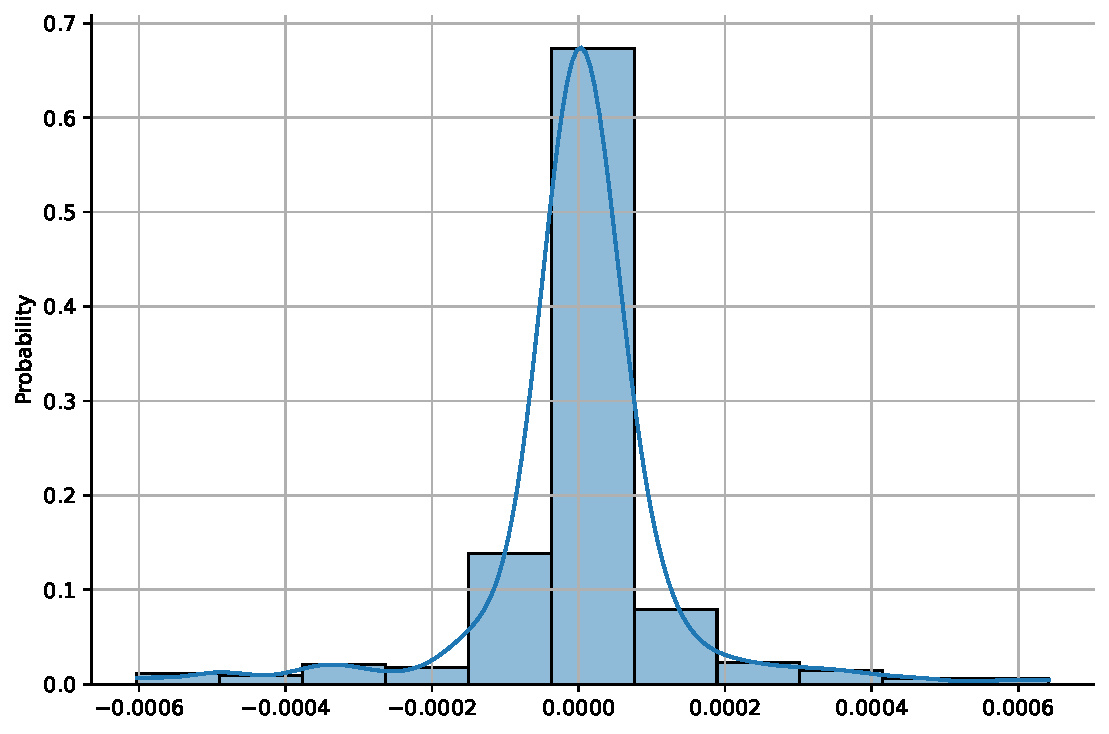
\includegraphics[width=0.5\textwidth]{1564ЛЕ1№1_п1_2500Гц-1Гц_1пФ_-10С_-4В-5В_10мВ_10мкс_шаг_0,01_multi_exp_hist}
		\caption{Гистограмма отклонений данных, полученных на идентифицированной 
		         модели, от экспериментальных данных. Сплошной линией показан 
		         результат сглаживания гистограммы.}
		\label{pic:multi_exp_hist_263}
	\end{figure}

	В таблице \ref{table:multi_exp_results_263} приведены параметры 
	идентифицированной модели и результаты оценок точности моделирования,  
	$\tau$ -- постоянная времени, $A$ -- амплитуда.

	\begin{table}[!htp]
    	\centering
    	\caption{Результаты идентификации модели.}
		\begin{tabular}{|l|l|l|l|}
			\hline
			Параметр                           & Значение & Параметр  & Значение  \\ \hline
			$\tau_1$, с                        & 0.000132 & $A_1$, пФ &  0.000301 \\ \hline
			$\tau_2$, с                        & 0.002744 & $A_2$, пФ &  0.000022 \\ \hline
			$\tau_3$, с                        & 0.001629 & $A_3$, пФ &  0.000102 \\ \hline
			$\tau_4$, с                        & 0.014347 & $A_4$, пФ & -0.000113 \\ \hline
			$\tau_5$, с                        & 0.017352 & $A_5$, пФ & -0.000135 \\ \hline
			$\tau_6$, с                        & 0.156241 & $A_6$, пФ & -0.000387 \\ \hline
			$\tau_7$, с                        & 0.001342 & $A_7$, пФ &  0.000139 \\ \hline
			$\tau_8$, с                        & 0.000230 & $A_8$, пФ &  0.000213 \\ \hline
			Результат кросвалидации (RMSE), пФ & 0.000134 &           &           \\ \hline
			RMSE, пФ                           & 0.000132 &           &           \\ \hline
		\end{tabular}
		\label{table:multi_exp_results_263}
	\end{table}

	На рисунке \ref{pic:multi_exp_spectr_263} приведён полученный спектр 
	частотного скана.

	\begin{figure}[!htp]
		\centering
		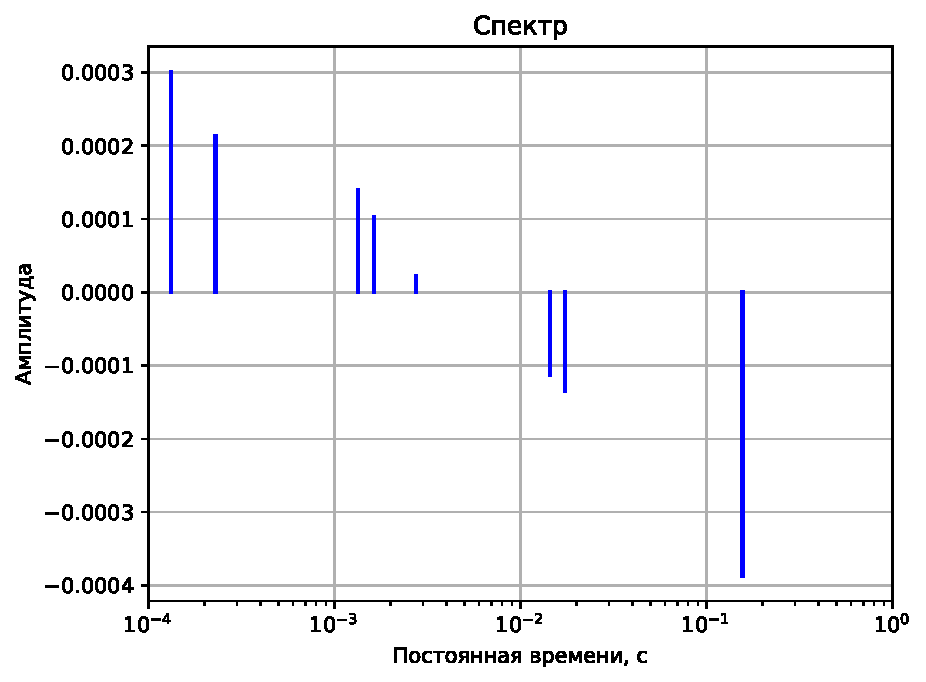
\includegraphics[width=0.5\textwidth]{1564ЛЕ1№1_п1_2500Гц-1Гц_1пФ_-10С_-4В-5В_10мВ_10мкс_шаг_0,01_multi_exp_spectr}
		\caption{Спектр сигнала релаксации ёмкости.}
		\label{pic:multi_exp_spectr_263}
	\end{figure}


	\newpage
	\subsubsection{Сравнение результатов}
	В таблице \ref{table:model_comparison_263} представлено сравнение результатов
	оценки точности рассмотренных моделей. В то время как модель идеального
	частотного скана (положительный пик) и модели c показателем $p$ показывают 
	приблизительно одинаковые результаты, многоэкспоненциальная модель показывает
	вдвое более высокую точность.
	
	\begin{table}[!htp]
	\centering
	\caption{Результаты идентификации моделей.}
	\begin{tabular}{|l|l|l|}
		\hline
		Модель                    & Результат         & RMSE, пФ \\ 
		                          & кросвалидации, пФ &          \\ \hline
		Идеаьный частотный скан   & 0.000279          & 0.000291 \\ \hline
		Модель с показателем $p$  & 0.000290          & 0.000291 \\
		(положительный пик)       &                   &          \\ \hline
		Модель с показателем $p$  & 0.000287          & 0.000286 \\ 
		(отрицательный пик)       &                   &          \\ \hline
		Многоэкспоененциальная    & 0.000134          & 0.000132 \\
		модель                    &                   &          \\ \hline
	\end{tabular}
	\label{table:model_comparison_263}
	\end{table}



	\newpage
	\subsection{Частотный скан при температуре 283 К}
	\subsubsection{Моноэкспоненциальная модель с показателем $p$}
	Результаты измерений при температуре 283~К приведены на рисунке 
	\ref{pic:train_data_283}. Полученный частотный скан имеет один пик,
	положительной полярности. Результаты идентификации модели с показателем 
	$p$ приведены на рисунке \ref{pic:single_exp_model_283}.

	\begin{figure}[!htp]
		\centering
		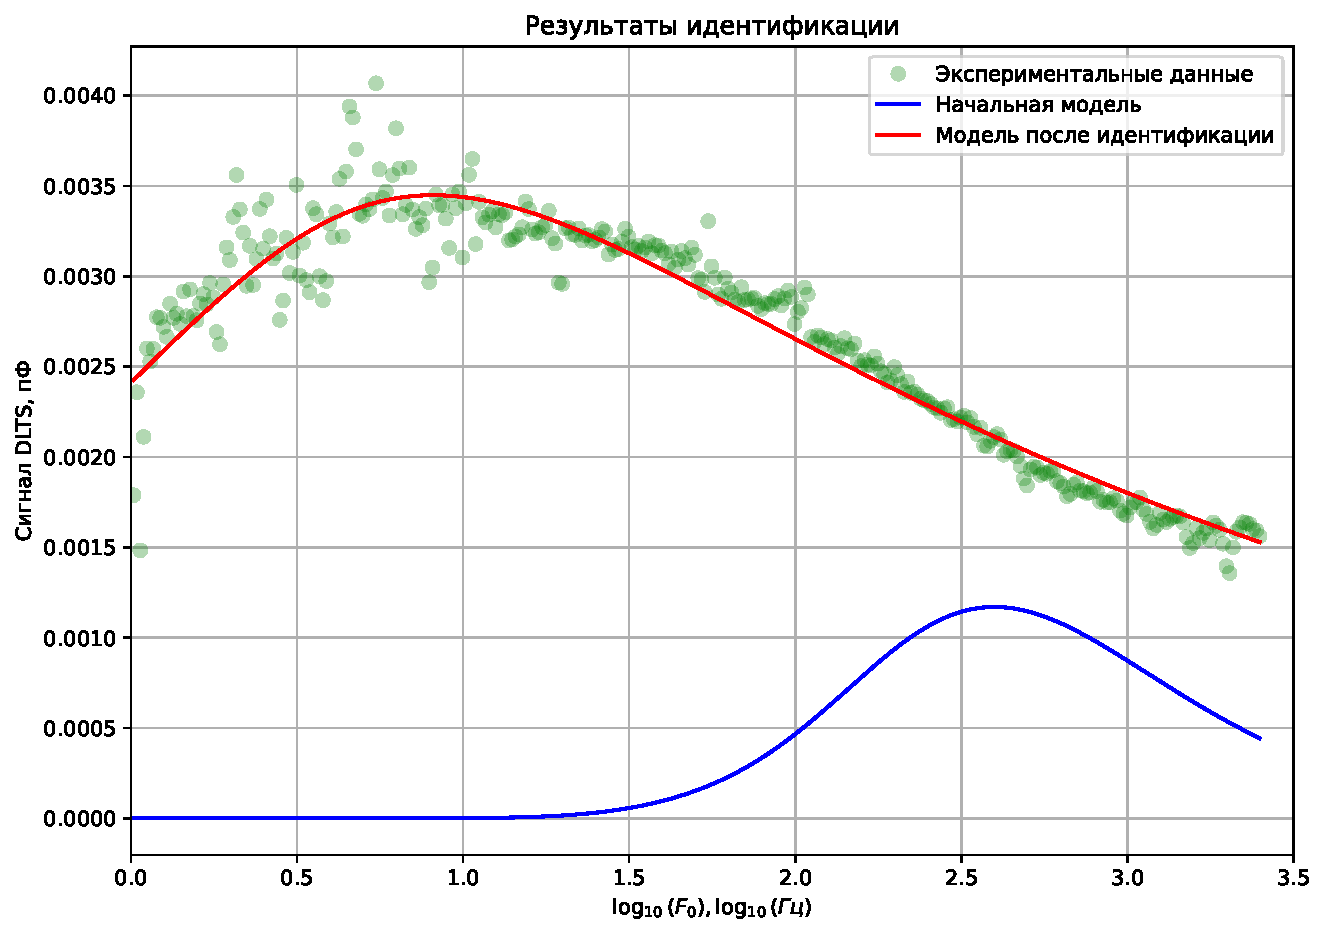
\includegraphics[width=0.75\textwidth]{1564ЛЕ1№1_п1_2500Гц-1Гц_1пФ_+10С_-4В-5В_50мВ_10мкс_шаг_0,01_single_exp_model}
		\caption{Результат идентификации частотного скана при $T=283K$.}
		\label{pic:single_exp_model_283}
	\end{figure}

	График нормированной среднеквадратической ошибки подтверждает на рисунке
	\ref{pic:loss_single_exp_283}, что алгоритм идентификации нашёл минимум 
	функции потерь.

	\begin{figure}[!htp]
		\centering
		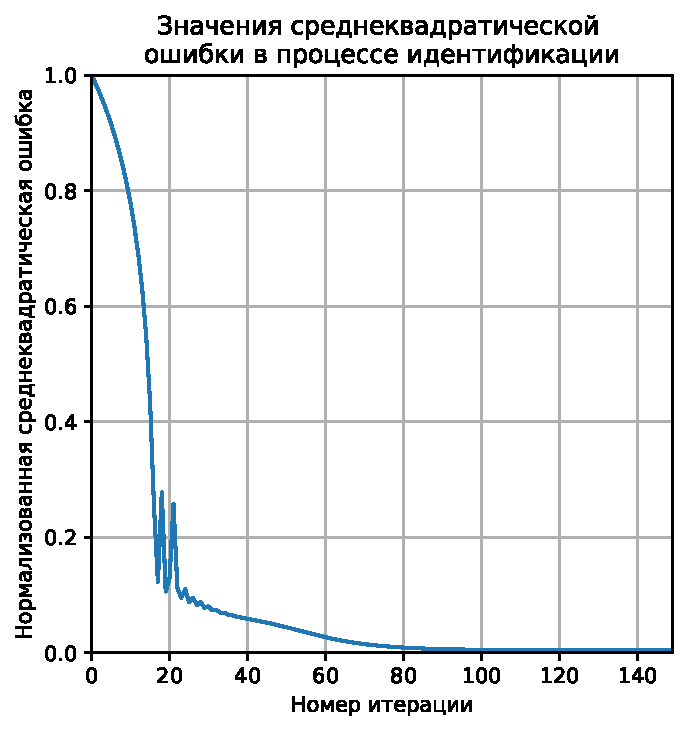
\includegraphics[width=0.35\textwidth]{1564ЛЕ1№1_п1_2500Гц-1Гц_1пФ_+10С_-4В-5В_50мВ_10мкс_шаг_0,01_single_exp_model_loss}
		\caption{График среднеквадратической ошибки в процессе идентификации,
		         нормированной относительно её максимального значения.}
		\label{pic:loss_single_exp_283}
	\end{figure}

	На рисунках \ref{pic:deviations_single_exp_283} и \ref{pic:hist_single_exp_283}
	показаны график отклонений результатов моделирования от экспериментальных
	данных и гистограмма отклонений. Гистограмма по форме близка к нормальному
	закону.

	\begin{figure}[!htp]
		\centering
		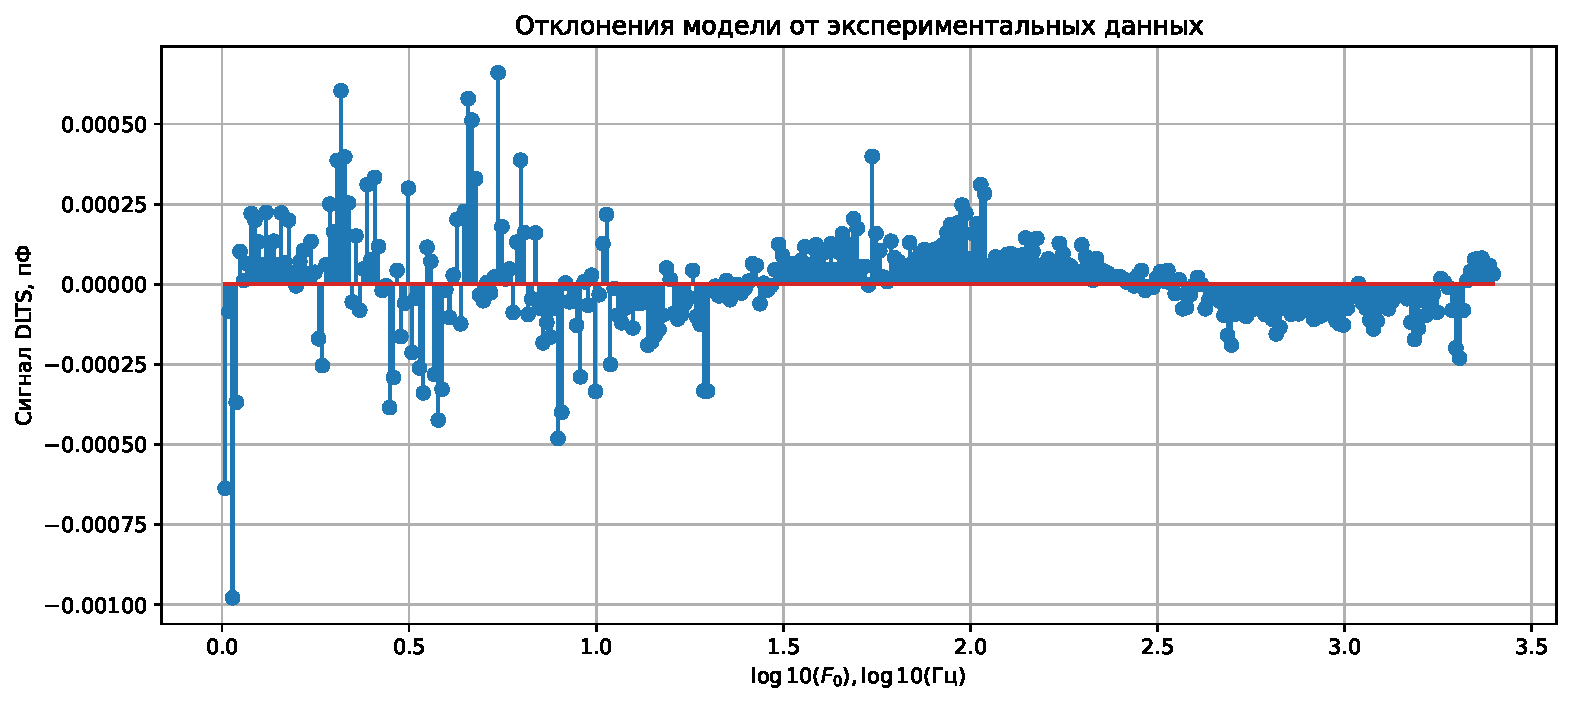
\includegraphics[width=0.75\textwidth]{1564ЛЕ1№1_п1_2500Гц-1Гц_1пФ_+10С_-4В-5В_50мВ_10мкс_шаг_0,01_single_exp_deviations}
		\caption{График отклонений результатов, полученных на идентифицированной
		модели, от экспериментальных данных.}
		\label{pic:deviations_single_exp_283}
	\end{figure}

	\begin{figure}[!htp]
		\centering
		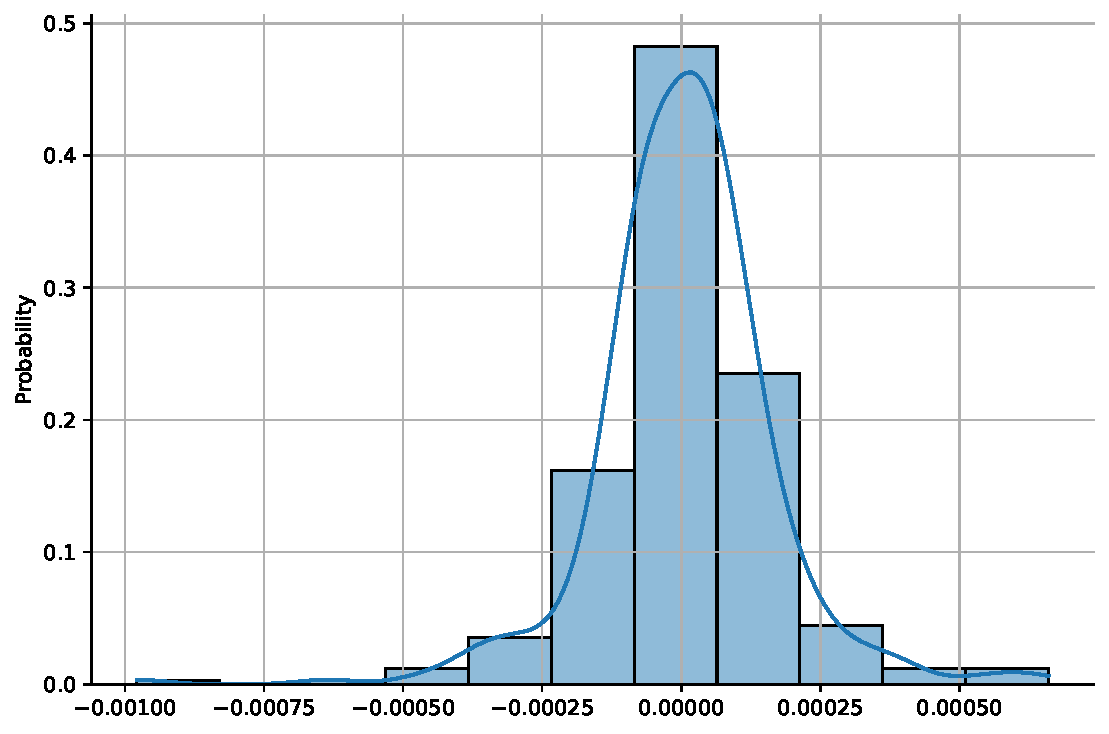
\includegraphics[width=0.5\textwidth]{1564ЛЕ1№1_п1_2500Гц-1Гц_1пФ_+10С_-4В-5В_50мВ_10мкс_шаг_0,01_single_exp_hist}
		\caption{Гистограмма отклонений данных, полученных на идентифицированной 
		         модели, от экспериментальных данных. Сплошной линией показан
		         результат сглаживания гистограммы.}
		\label{pic:hist_single_exp_283}
	\end{figure}

	В таблице \ref{table:results_single_exp_283} приведены параметры 
	идентифицированной модели и результаты оценок точности моделирования.

	\begin{table}[!htp]
		\centering
		\caption{Результаты идентификации модели}
		\begin{tabular}{|l|l|}
			\hline
			Параметр                           & Значение \\ \hline
			Постоянна времени $\tau$, с        & 0,054291 \\ \hline
			Амплитуда, пФ                      & 0.003448 \\ \hline
			Показатель $p$                     & 0.173    \\ \hline
			Результат кросвалидации (RMSE), пФ & 0.000160 \\ \hline
			RMSE, пФ                           & 0.000161 \\ \hline
		\end{tabular}
		\label{table:results_single_exp_283}
	\end{table}

	На рисунке \ref{pic:multi_exp_spectr_283} приведён полученный спектр 
	частотного скана.

	\begin{figure}[!htp]
		\centering
		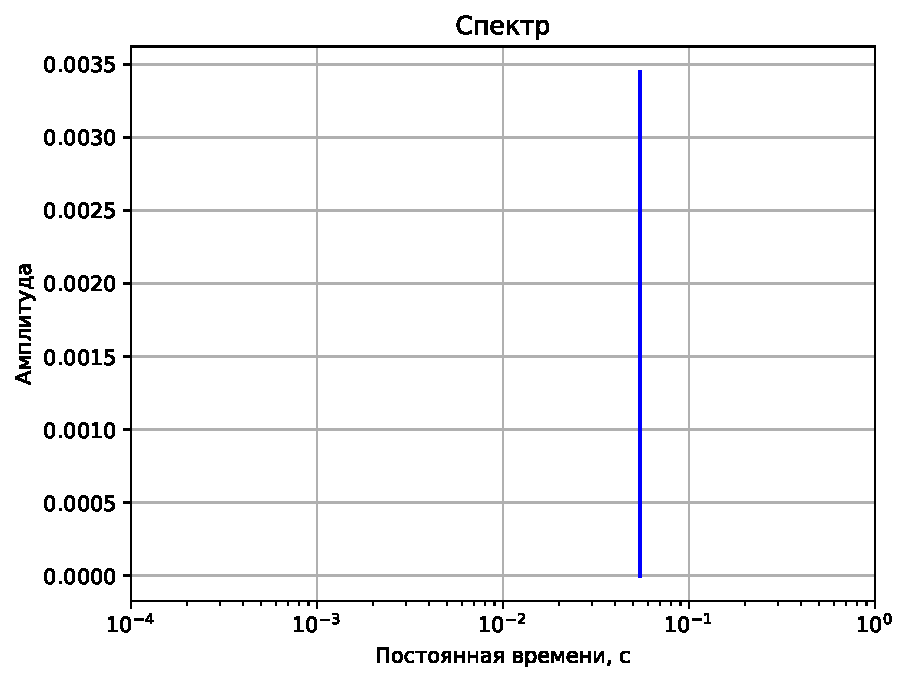
\includegraphics[width=0.5\textwidth]{1564ЛЕ1№1_п1_2500Гц-1Гц_1пФ_+10С_-4В-5В_50мВ_10мкс_шаг_0,01_single_exp_spectr}
		\caption{Спектр сигнала релаксации ёмкости.}
		\label{pic:spectr_single_exp_283}
	\end{figure}


	\newpage
	\subsubsection{Моноэкспоненциальная модель с показателем $p = 1$}

	Выполним идентификацию модели идеального частотного скана на результатах,
	полученных при температуре 283~К. Результаты идентификации модели приведены 
	на рисунке \ref{pic:model_single_exp_ideal_283}. На графике заметны
	существенные отклонения результатов моделирования от экспериментальных 
	данных, при этом, график значений нормированной среднеквадратической ошибки
	для каждой итерации (рисунок \ref{pic:loss_single_exp_ideal_283}) 
	свидетельствует о том, что алгоритм идентификации нашёл минимум функции 
	потерь.

	\begin{figure}[!htp]
		\centering
		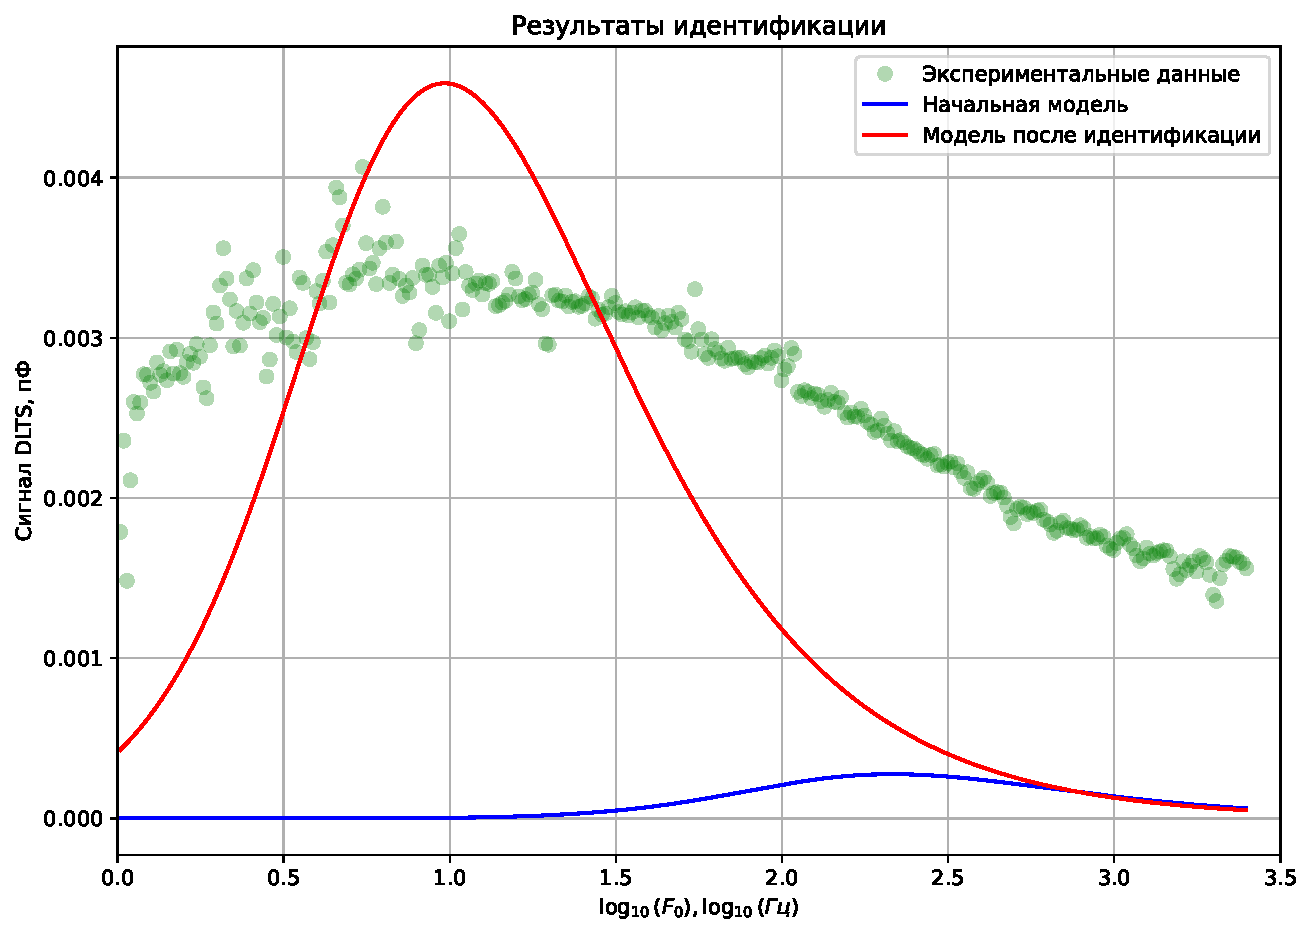
\includegraphics[width=0.75\textwidth]{1564ЛЕ1№1_п1_2500Гц-1Гц_1пФ_+10С_-4В-5В_50мВ_10мкс_шаг_0,01_single_exp_ideal_model}
		\caption{Результат идентификации частотного скана при $T=283K$.}
		\label{pic:model_single_exp_ideal_283}
	\end{figure}

	\begin{figure}[!htp]
		\centering
		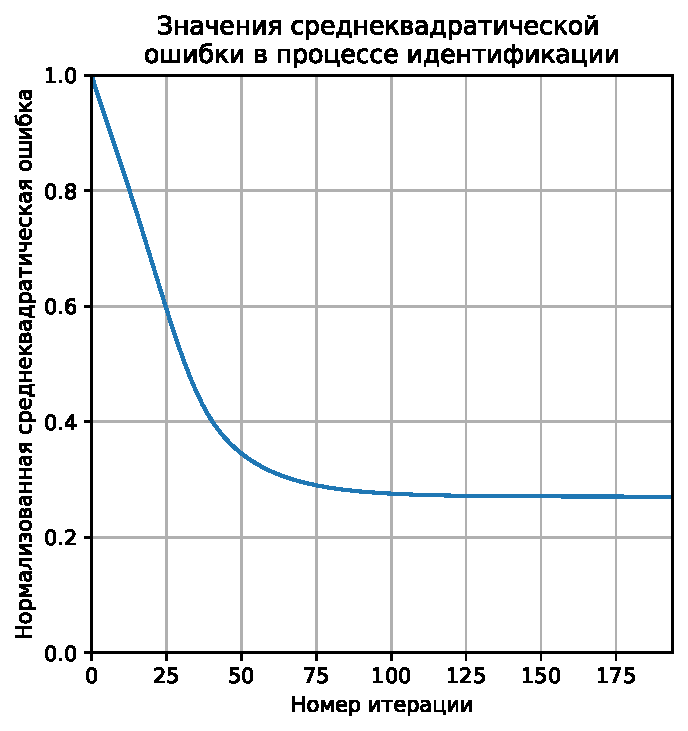
\includegraphics[width=0.35\textwidth]{1564ЛЕ1№1_п1_2500Гц-1Гц_1пФ_+10С_-4В-5В_50мВ_10мкс_шаг_0,01_single_exp_ideal_model_loss}
		\caption{График среднеквадратической ошибки в процессе идентификации,
		         нормированной относительно её максимального значения.}
		\label{pic:loss_single_exp_ideal_283}
	\end{figure}

	График отклонений результатов моделирования от экспериментальных данных 
	(рисунок \ref{pic:deviations_single_exp_ideal_283}) также демонстрирует
	значительные систематические отклонения. Закономерно, гистограмма (рисунок
	\ref{pic:hist_single_exp_ideal_283}) по форме далека от нормального
	распределения.

	\begin{figure}[!htp]
		\centering
		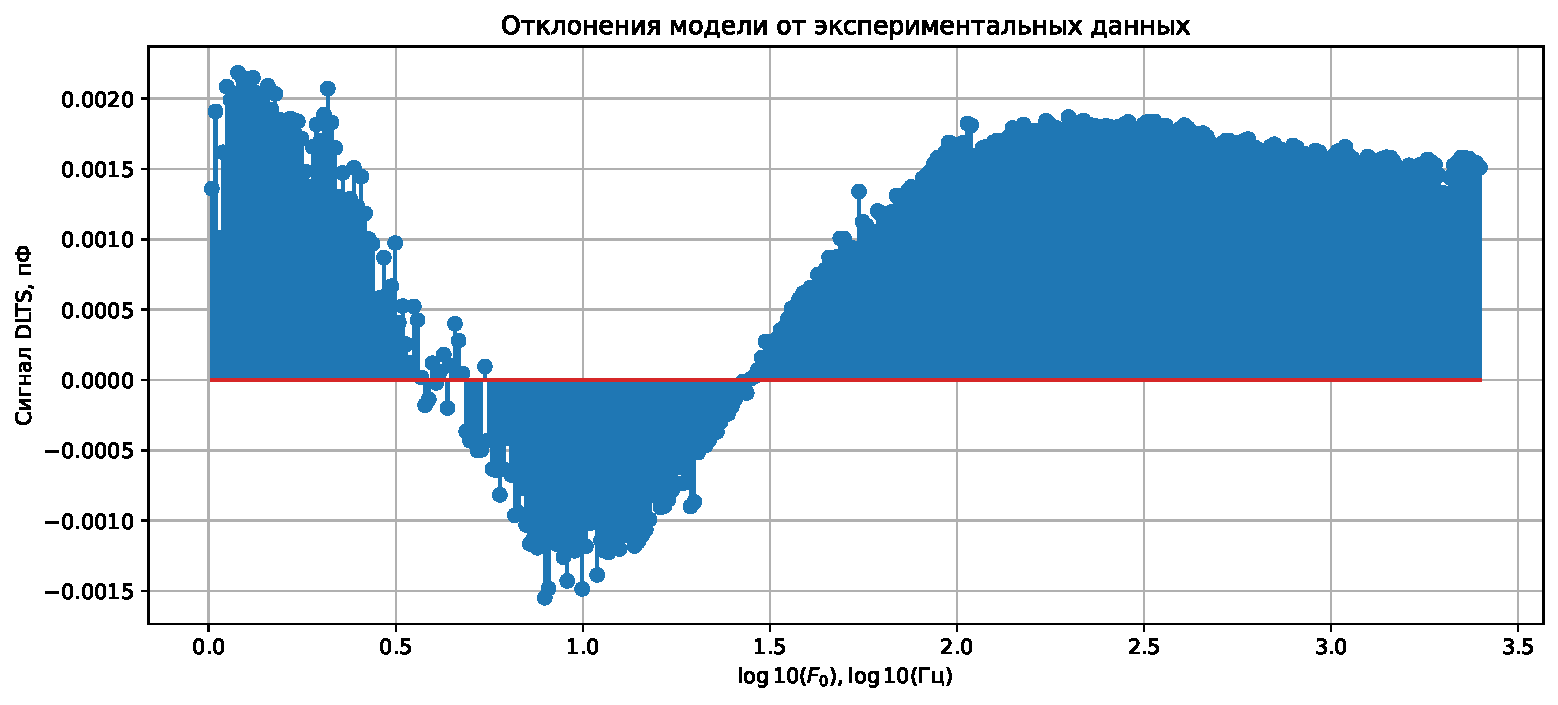
\includegraphics[width=0.75\textwidth]{1564ЛЕ1№1_п1_2500Гц-1Гц_1пФ_+10С_-4В-5В_50мВ_10мкс_шаг_0,01_single_exp_ideal_deviations}
		\caption{График отклонений результатов, полученных на идентифицированной
		модели, от экспериментальных данных.}
		\label{pic:deviations_single_exp_ideal_283}
	\end{figure}

	\begin{figure}[!htp]
		\centering
		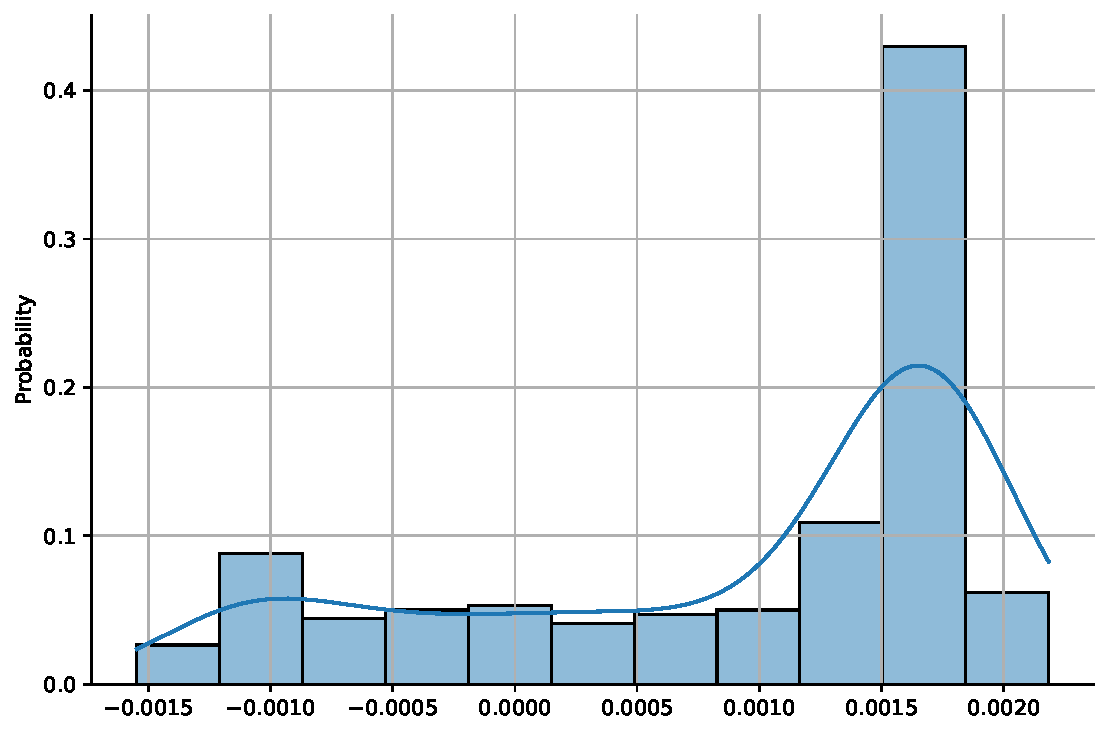
\includegraphics[width=0.5\textwidth]{1564ЛЕ1№1_п1_2500Гц-1Гц_1пФ_+10С_-4В-5В_50мВ_10мкс_шаг_0,01_single_exp_ideal_hist}
		\caption{Гистограмма отклонений данных, полученных на идентифицированной 
		         модели, от экспериментальных данных. Сплошной линией показан
		         результат сглаживания гистограммы.}
		\label{pic:hist_single_exp_ideal_283}
	\end{figure}

	В таблице \ref{table:results_single_exp_ideal_283} приведены параметры 
	идентифицированной модели и результаты оценок точности моделирования.

	\begin{table}[!htp]
		\centering
		\caption{Результаты идентификации модели}
		\begin{tabular}{|l|l|}
			\hline
			Параметр                           & Значение \\ \hline
			Постоянна времени $\tau$, с        & 0.045708 \\ \hline
			Амплитуда, пФ                      & 0.004591 \\ \hline
			Показатель $p$                     & 1.0      \\ \hline
			Результат кросвалидации (RMSE), пФ & 0.001396 \\ \hline
			RMSE, пФ                           & 0.001389 \\ \hline
		\end{tabular}
		\label{table:results_single_exp_ideal_283}
	\end{table}

	На рисунке \ref{pic:spectr_single_exp_ideal_283} приведён полученный спектр 
	частотного скана.

	\begin{figure}[!htp]
		\centering
		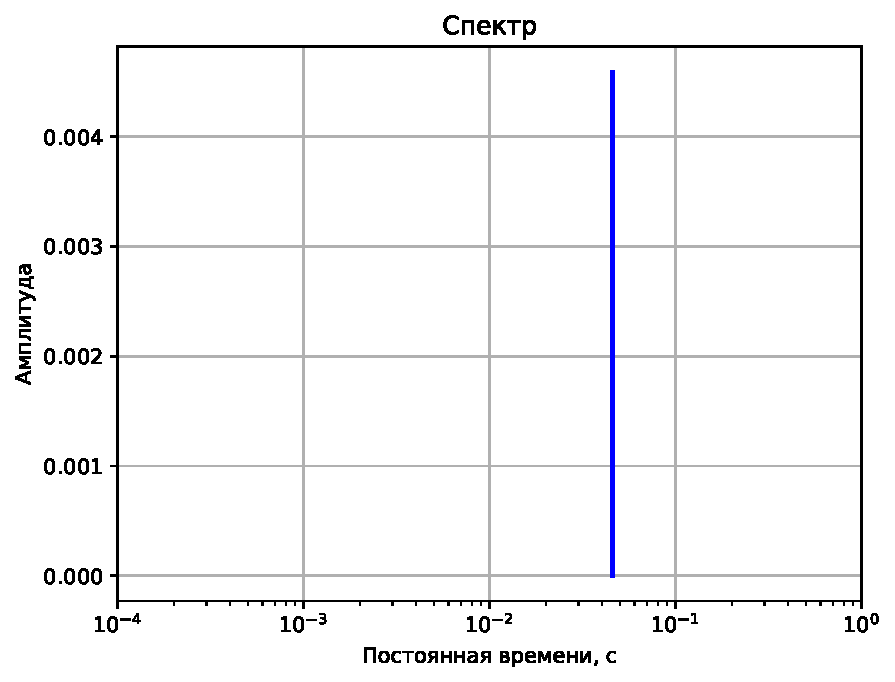
\includegraphics[width=0.5\textwidth]{1564ЛЕ1№1_п1_2500Гц-1Гц_1пФ_+10С_-4В-5В_50мВ_10мкс_шаг_0,01_single_exp_ideal_spectr}
		\caption{Спектр сигнала релаксации ёмкости.}
		\label{pic:spectr_single_exp_ideal_283}
	\end{figure}


	\newpage
	\subsubsection{Многоэкспоненциальная модель с n\_exps > 1}
	Выполним идентификацию многоэкспоненциальной модели, для этого сравним
	результаты кросвалидации для моделей, имеющих значения парамера n\_exps
	равные 5, 6, 7, 8, 9 и 10, и выберем показавшую лучший результат. В таблице
	\ref{table:multi_exp_model_283_cross_val} представлены полученные результаты.
	Лучшей оказалась модель с параметром n\_exps = 6, то есть имеющая 6 
	экспоненциальных составляющих.

	\begin{table}[!htp]
		\centering
		\caption{Результаты кросвалидации для разных значений параметра n\_exps}
		\begin{tabular}{|l|l|}
		\hline
		Значение параметра n\_exps & Результат кросвалидации \\ \hline
		5                          & 0.0001579               \\ \hline
		6                          & 0.0001530               \\ \hline
		7                          & 0.0001532               \\ \hline
		8                          & 0.0001547               \\ \hline
		9                          & 0.0001537               \\ \hline
		10                         & 0.0001546               \\ \hline
		\end{tabular}
		\label{table:multi_exp_model_283_cross_val}
	\end{table}

	Результаты идентификации модели с шестью экспоненциальными составляющими
	представлены на рисунке \ref{pic:multi_exp_model_283}.

	\begin{figure}[!htp]
		\centering
		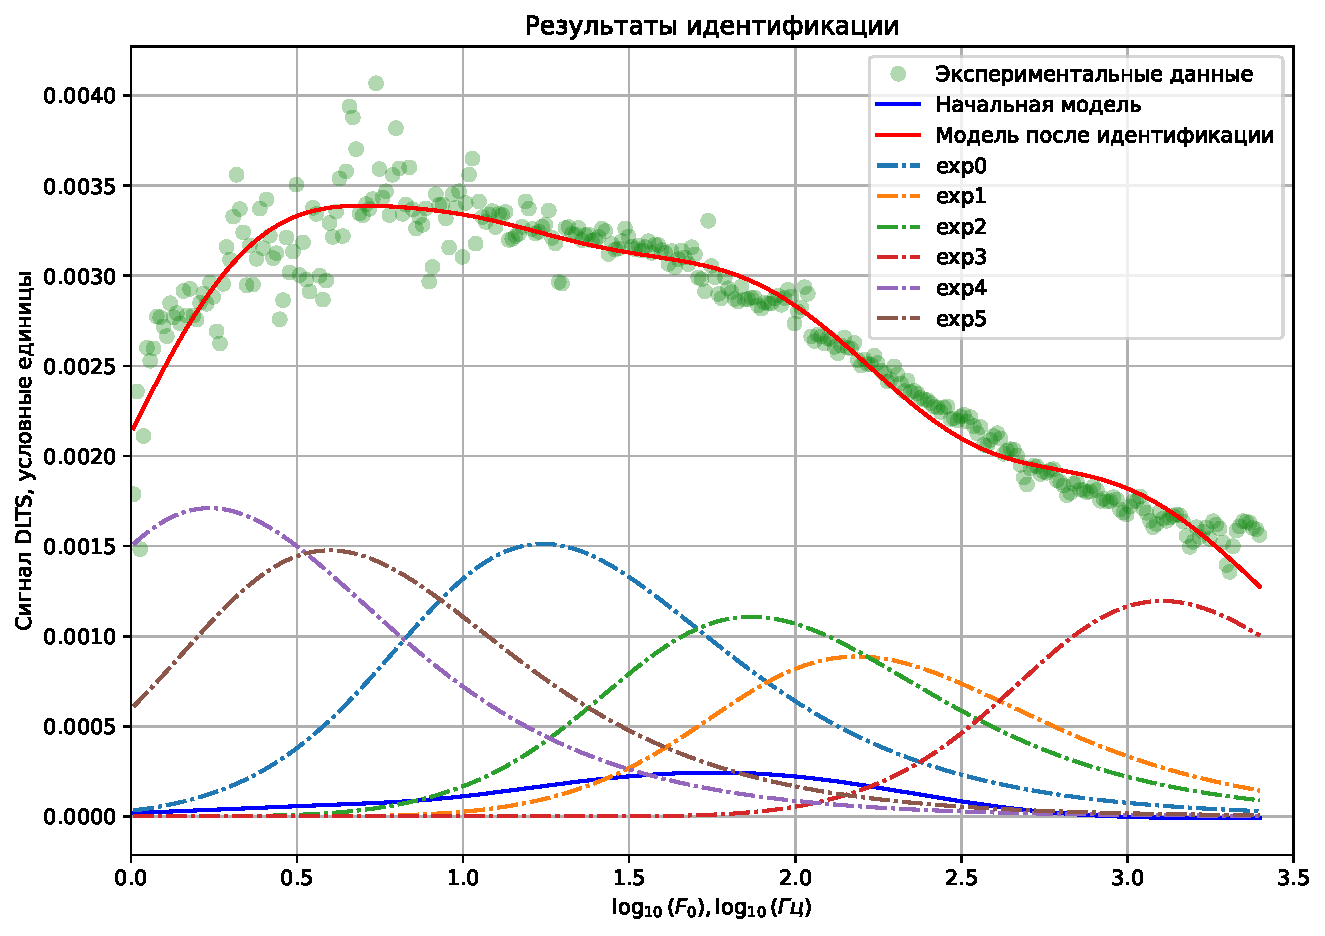
\includegraphics[width=0.75\textwidth]{1564ЛЕ1№1_п1_2500Гц-1Гц_1пФ_+10С_-4В-5В_50мВ_10мкс_шаг_0,01_multi_exp_model}
		\caption{Результат идентификации многоэкспоненциальной моделью 
		         частотного скана при $T=283K$.}
		\label{pic:multi_exp_model_283}
	\end{figure}

	На рисунке \ref{pic:multi_exp_loss_283} показан график нормированной
	среднеквадратической ошибки. Форма графика говорит о том, что алгоритм
	идентификации нашёл минимум функции потерь.

	\begin{figure}[!htp]
		\centering
		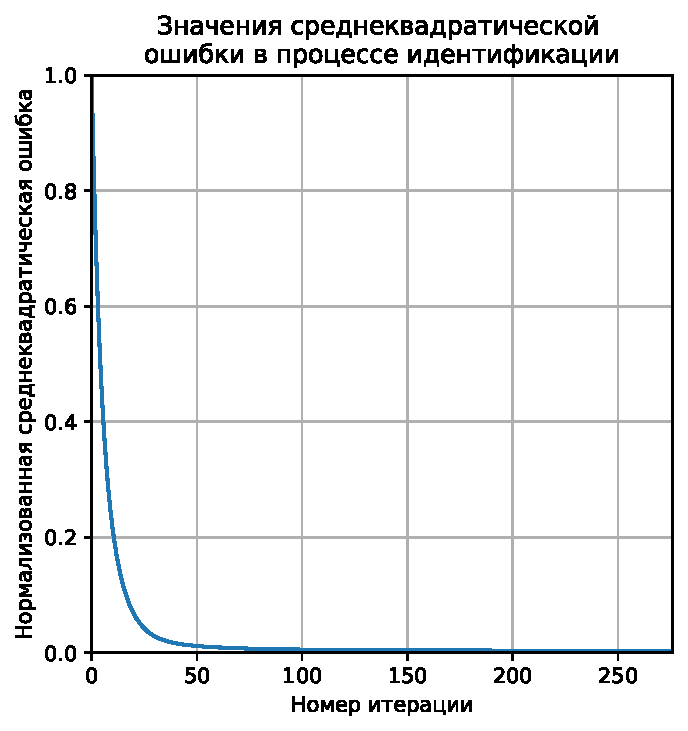
\includegraphics[width=0.35\textwidth]{1564ЛЕ1№1_п1_2500Гц-1Гц_1пФ_+10С_-4В-5В_50мВ_10мкс_шаг_0,01_multi_exp_loss}
		\caption{График среднеквадратической ошибки в процессе идентификации,
		         нормированной относительно её максимального значения.}
		\label{pic:multi_exp_loss_283}
	\end{figure}

	На графике отклонений результатов моделирования от экспериментальных данных
	(рисунок \ref{pic:multi_exp_deviations_283}) заметны систематические отклонения
	в области высоких значенией частоты опорной функции. Они же заметны на 
	рисунке \ref{pic:multi_exp_model_283}. Их появление может быть связано с 
	влиянием случайной инициализации модели -- алгоритм из-за <<неудачных>> 
	начальных значений завершил работу вблизи минимума функции потерь, но
	самого минимума так и не достиг.

	\begin{figure}[!htp]
		\centering
		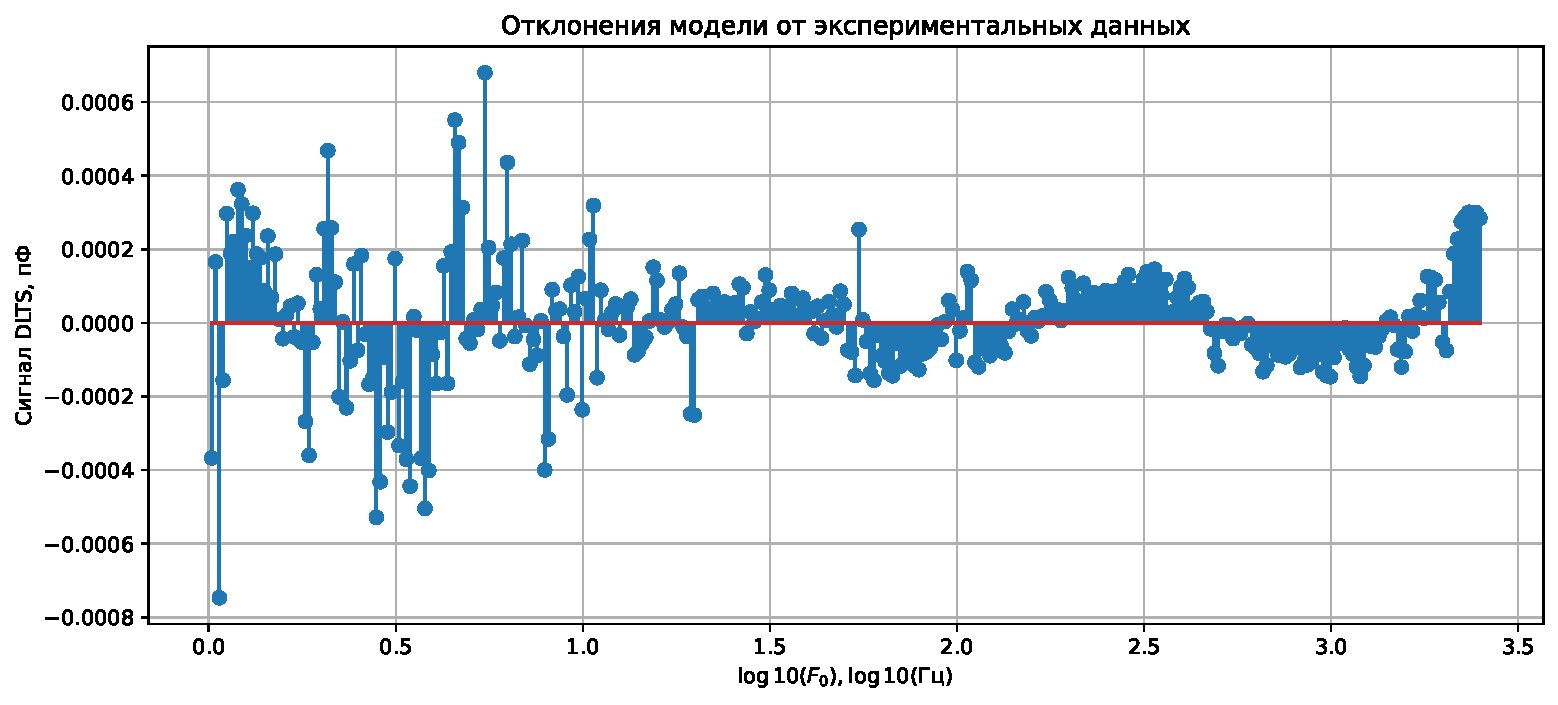
\includegraphics[width=0.75\textwidth]{1564ЛЕ1№1_п1_2500Гц-1Гц_1пФ_+10С_-4В-5В_50мВ_10мкс_шаг_0,01_multi_exp_deviations}
		\caption{График отклонений результатов, полученных на идентифицированной
		модели, от экспериментальных данных.}
		\label{pic:multi_exp_deviations_283}
	\end{figure}

	На рисунке \ref{pic:multi_exp_hist_283} показана гистограмма отклонений 
	результатов моделирования от экспериментальных данных. Форма гистограммы 
	близка к форме нормального распределения.

	\begin{figure}[!htp]
		\centering
		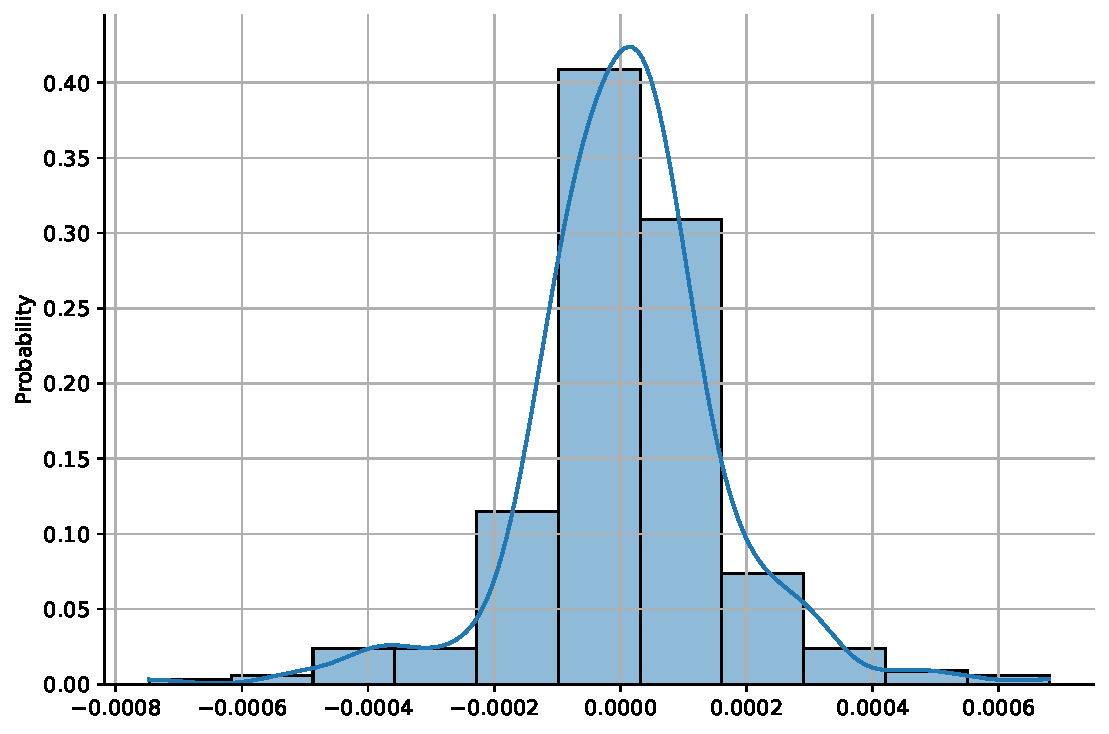
\includegraphics[width=0.5\textwidth]{1564ЛЕ1№1_п1_2500Гц-1Гц_1пФ_+10С_-4В-5В_50мВ_10мкс_шаг_0,01_multi_exp_hist}
		\caption{Гистограмма отклонений данных, полученных на идентифицированной 
		         модели, от экспериментальных данных. Сплошной линией показан
		         результат сглаживания гистограммы.}
		\label{pic:multi_exp_hist_283}
	\end{figure}

	В таблице \ref{table:multi_exp_results_283} приведены параметры 
	идентифицированной модели и результаты оценок точности моделирования,  
	$\tau$ -- постоянная времени, $A$ -- амплитуда.

	\begin{table}[!htp]
		\centering
		\caption{Результаты идентификации модели.}
		\begin{tabular}{|l|l|l|l|}
			\hline
			Параметр                           & Значение & Параметр  & Значение  \\ \hline
			$\tau_1$, с                        & 0.025388 & $A_1$, пФ & 0.001513  \\ \hline
			$\tau_2$, с                        & 0.002868 & $A_2$, пФ & 0.000887  \\ \hline
			$\tau_3$, с                        & 0.005958 & $A_3$, пФ & 0.001108  \\ \hline
			$\tau_4$, с                        & 0.000336 & $A_4$, пФ & 0.001196  \\ \hline
			$\tau_5$, с                        & 0.255645 & $A_5$, пФ & 0.001711  \\ \hline
			$\tau_6$, с                        & 0.111247 & $A_6$, пФ & 0.001476  \\ \hline
			Результат кросвалидации (RMSE), пФ & 0.000158 &           &           \\ \hline
			RMSE, пФ                           & 0.000156 &           &           \\ \hline
		\end{tabular}
		\label{table:multi_exp_results_283}
	\end{table}

	На рисунке \ref{pic:multi_exp_spectr_283} приведён полученный спектр 
	частотного скана.

	\begin{figure}[!htp]
		\centering
		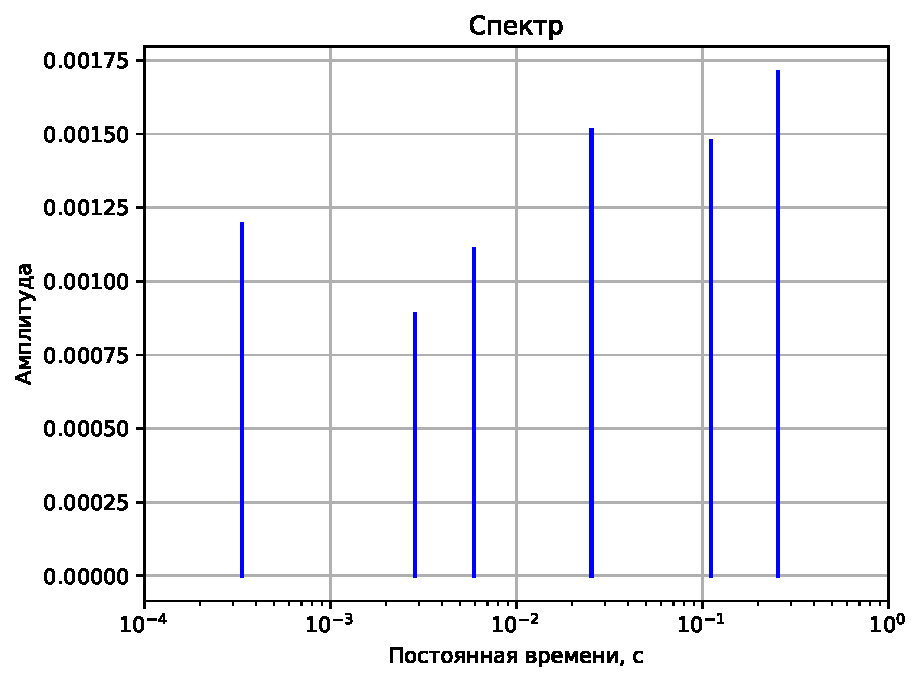
\includegraphics[width=0.5\textwidth]{1564ЛЕ1№1_п1_2500Гц-1Гц_1пФ_+10С_-4В-5В_50мВ_10мкс_шаг_0,01_multi_exp_spectr}
		\caption{Спектр сигнала релаксации ёмкости.}
		\label{pic:multi_exp_spectr_283}
	\end{figure}


	\newpage
	\subsubsection{Сравнение результатов}
	В таблице \ref{table:model_comparison_283} представлено сравнение результатов
	оценки точности рассмотренных моделей. 

	Модель идеального частотного скана демонстрирует значительные отклонения от
	результатов измерений, и, скорее всего, не подходит для описания экспериментальных
	данных, в то время как модель с показателем $p$ и многоэкспоненциальная модель
	неплохо согласуются с результатами измерений и показывают примерно одинаковую
	точность. 
	
	\begin{table}[!htp]
	\centering
	\caption{Результаты идентификации моделей.}
	\begin{tabular}{|l|l|l|}
		\hline
		Модель                    & Результат         & RMSE, пФ \\ 
		                          & кросвалидации, пФ &          \\ \hline
		Идеаьный частотный скан   & 0.001396          & 0.001389 \\ \hline
		Модель с показателем $p$  & 0.000160          & 0.000161 \\ \hline
		Многоэкспоененциальная    & 0.000158          & 0.000156 \\
		модель                    &                   &          \\ \hline
	\end{tabular}
	\label{table:model_comparison_283}
	\end{table}



	\newpage
	\subsection{Частотный скан при температуре 303 К}
	\subsubsection{Моноэкспоненциальная модель с показателем $p$}
	Результаты измерений при температуре 303~К приведены на рисунке 
	\ref{pic:train_data_303}. К сожалению, частотный скан содержит всего 34 точки,
	поэтому гистограммы и графики отклонений будут не так информативны как в 
	предыдущих разделах. Результаты идентификации моноэкспоненциальной модели 
	с показателем $p$ приведены на рисунке \ref{pic:model_single_exp_303}.

	\begin{figure}[!htp]
		\centering
		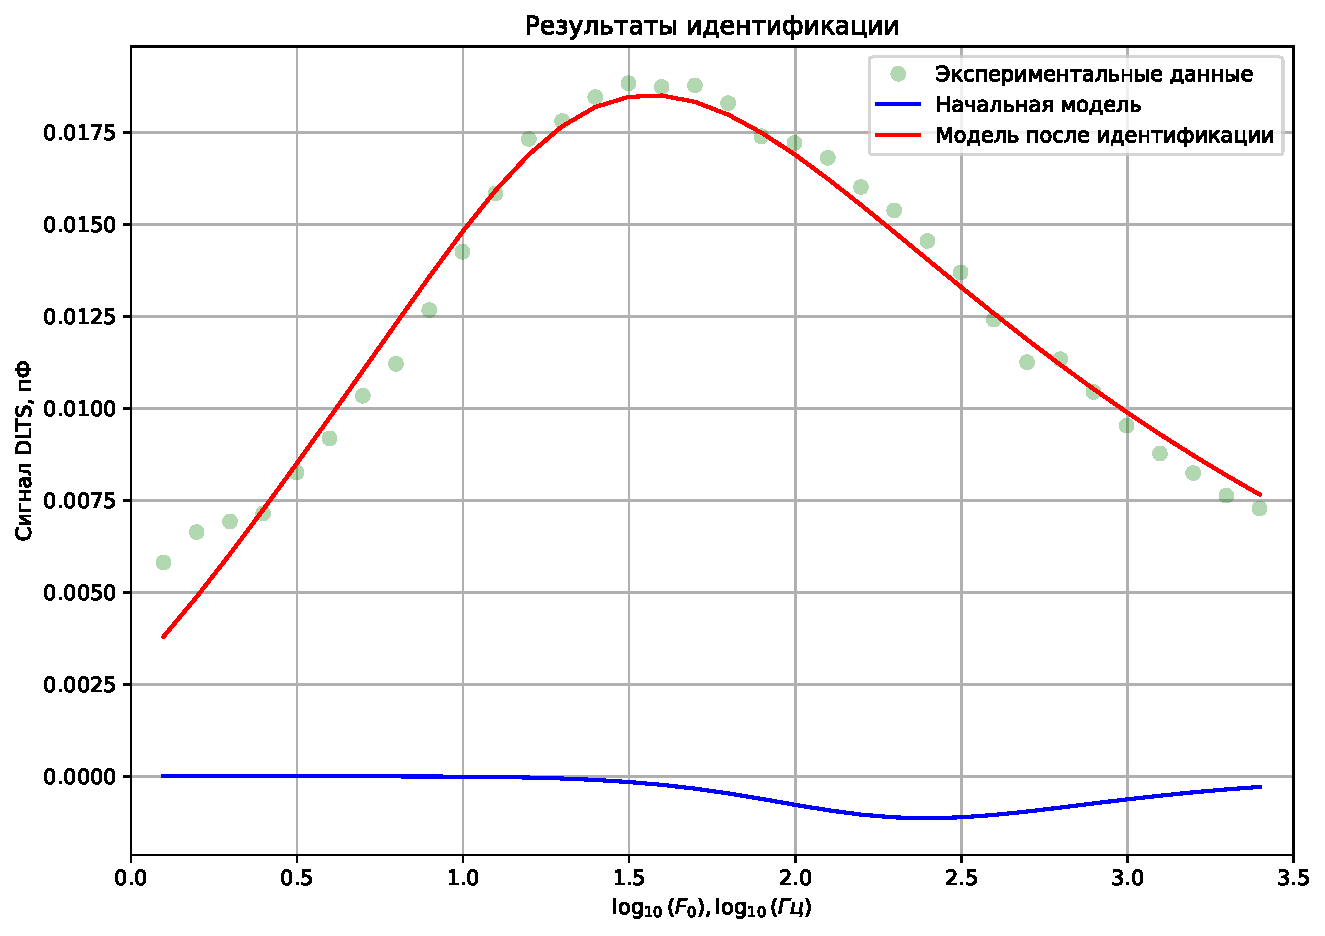
\includegraphics[width=0.75\textwidth]{1564ЛЕ1№1_п1_2500Гц-1Гц_10пФ_+30С_-4В-5В_50мВ_10мкс_шаг_0,1_single_exp_model}
		\caption{Результат идентификации положительного пика частотного скана
		         при $T=303K$.}
		\label{pic:model_single_exp_303}
	\end{figure}

	График нормированной среднеквадратической ошибки, приведенный на рисунке
	\ref{pic:loss_single_exp_303}, указывает на то, что алгоритм идентификации
	нашёл минимум функции потерь.

	\begin{figure}[!htp]
		\centering
		\includegraphics[width=0.35\textwidth]{1564ЛЕ1№1_п1_2500Гц-1Гц_10пФ_+30С_-4В-5В_50мВ_10мкс_шаг_0,1_single_exp_model_loss}
		\caption{График среднеквадратической ошибки в процессе идентификации,
		         нормированной относительно её максимального значения.}
		\label{pic:loss_single_exp_303}
	\end{figure}

	На графике отклонений результатов моделирования, полученных на идентифицированной
	модели, от экспериментальных данных (рисунок \ref{pic:deviations_single_exp_303})
	заметны систематические отклонения. Гистограмма отклонений, приведённая на 
	рисунке \ref{pic:hist_single_exp_303}, по форме существенно отличается от
	нормального распределения.

	\begin{figure}[!htp]
		\centering
		\includegraphics[width=0.75\textwidth]{1564ЛЕ1№1_п1_2500Гц-1Гц_10пФ_+30С_-4В-5В_50мВ_10мкс_шаг_0,1_single_exp_deviations}
		\caption{График отклонений результатов, полученных на идентифицированной
		модели, от экспериментальных данных.}
		\label{pic:deviations_single_exp_303}
	\end{figure}

	\begin{figure}[!htp]
		\centering
		\includegraphics[width=0.5\textwidth]{1564ЛЕ1№1_п1_2500Гц-1Гц_10пФ_+30С_-4В-5В_50мВ_10мкс_шаг_0,1_single_exp_hist}
		\caption{Гистограмма отклонений данных, полученных на идентифицированной 
		         модели, от экспериментальных данных. Сплошной линией показан
		         результат сглаживания гистограммы.}
		\label{pic:hist_single_exp_303}
	\end{figure}

	В таблице \ref{table:results_single_exp_303} приведены параметры 
	идентифицированной модели и результаты оценок точности моделирования.

	\begin{table}[!htp]
		\centering
		\caption{Результаты идентификации модели}
		\begin{tabular}{|l|l|}
			\hline
			Параметр                           & Значение \\ \hline
			Постоянна времени $\tau$, с        & 0,012014 \\ \hline
			Амплитуда, пФ                      & 0.018520 \\ \hline
			Показатель $p$                     & 0.275712 \\ \hline
			Результат кросвалидации (RMSE), пФ & 0.000713 \\ \hline
			RMSE, пФ                           & 0.000660 \\ \hline
		\end{tabular}
		\label{table:results_single_exp_303}
	\end{table}

	На рисунке \ref{pic:spectr_single_exp_303} приведён полученный спектр 
	частотного скана.

	\begin{figure}[!htp]
		\centering
		\includegraphics[width=0.5\textwidth]{1564ЛЕ1№1_п1_2500Гц-1Гц_1пФ_+30С_-4В-5В_50мВ_10мкс_шаг_0,01_single_exp_spectr}
		\caption{Спектр сигнала релаксации ёмкости.}
		\label{pic:spectr_single_exp_303}
	\end{figure}


	\newpage
	\subsubsection{Моноэкспоненциальная модель с показателем $p=1$}
	Выполним идентификацию модели идеального частотного скана на результатах,
	полученных при температуре 303~К. Результаты идентификации модели приведены 
	на рисунке \ref{pic:model_single_exp_ideal_303}. На графике заметны
	существенные отклонения результатов моделирования от экспериментальных 
	данных, при этом, график значений нормированной среднеквадратической ошибки
	для каждой итерации (рисунок \ref{pic:loss_single_exp_ideal_303}) 
	свидетельствует о том, что алгоритм идентификации нашёл минимум функции 
	потерь.

	\begin{figure}[!htp]
		\centering
		\includegraphics[width=0.75\textwidth]{1564ЛЕ1№1_п1_2500Гц-1Гц_10пФ_+30С_-4В-5В_50мВ_10мкс_шаг_0,1_single_exp_ideal_model}
		\caption{Результат идентификации положительного пика частотного скана
		         при $T=303K$.}
		\label{pic:model_single_exp_ideal_303}
	\end{figure}

	\begin{figure}[!htp]
		\centering
		\includegraphics[width=0.35\textwidth]{1564ЛЕ1№1_п1_2500Гц-1Гц_10пФ_+30С_-4В-5В_50мВ_10мкс_шаг_0,1_single_exp_ideal_model_loss}
		\caption{График среднеквадратической ошибки в процессе идентификации,
		         нормированной относительно её максимального значения.}
		\label{pic:loss_single_exp_ideal_303}
	\end{figure}

	График отклонений результатов моделирования от экспериментальных данных
	(рисунок \ref{pic:deviations_single_exp_ideal_303}) также демонстрирует
	значительные систематические отклонения, а гистограмма (рисунок 
	\ref{pic:hist_single_exp_ideal_303}) по форме далека от нормального 
	распределения.

	\begin{figure}[!htp]
		\centering
		\includegraphics[width=0.75\textwidth]{1564ЛЕ1№1_п1_2500Гц-1Гц_10пФ_+30С_-4В-5В_50мВ_10мкс_шаг_0,1_single_exp_ideal_deviations}
		\caption{График отклонений результатов, полученных на идентифицированной
		модели, от экспериментальных данных.}
		\label{pic:deviations_single_exp_ideal_303}
	\end{figure}

	\begin{figure}[!htp]
		\centering
		\includegraphics[width=0.5\textwidth]{1564ЛЕ1№1_п1_2500Гц-1Гц_10пФ_+30С_-4В-5В_50мВ_10мкс_шаг_0,1_single_exp_ideal_hist}
		\caption{Гистограмма отклонений данных, полученных на идентифицированной 
		         модели, от экспериментальных данных.Сплошной линией показан
		         результат сглаживания гистограммы.}
		\label{pic:hist_single_exp_ideal_303}
	\end{figure}

	В таблице \ref{table:results_single_exp_ideal_303} приведены параметры 
	идентифицированной модели и результаты оценок точности моделирования.

	\begin{table}[!htp]
		\centering
		\caption{Результаты идентификации модели}
		\begin{tabular}{|l|l|}
			\hline
			Параметр                           & Значение \\ \hline
			Постоянна времени $\tau$, с        & 0,011709 \\ \hline
			Амплитуда, пФ                      & 0.023837 \\ \hline
			Показатель $p$                     & 1.0      \\ \hline
			Результат кросвалидации (RMSE), пФ & 0.005837 \\ \hline
			RMSE, пФ                           & 0.005436 \\ \hline
		\end{tabular}
		\label{table:results_single_exp_ideal_303}
	\end{table}

	На рисунке \ref{pic:spectr_single_exp_ideal_303} приведён полученный спектр
	частотного скана.

	\begin{figure}[!htp]
		\centering
		\includegraphics[width=0.5\textwidth]{1564ЛЕ1№1_п1_2500Гц-1Гц_10пФ_+30С_-4В-5В_50мВ_10мкс_шаг_0,1_single_exp_ideal_spectr}
		\caption{Спектр сигнала релаксации ёмкости.}
		\label{pic:spectr_single_exp_ideal_303}
	\end{figure}


	\newpage
	\subsubsection{Многоэкспоненциальная модель с n\_exps > 1}
	Выполним идентификацию многоэкспоненциальной модели, для этого сравним
	результаты кросвалидации для моделей, имеющих значения парамера n\_exps
	равные 5, 6, 7, 8, 9 и 10, и выберем показавшую лучший результат. В таблице
	\ref{table:multi_exp_model_303_cross_val} представлены полученные результаты.
	Лучшей оказалась модель с параметром n\_exps = 6, то есть имеющая 6 
	экспоненциальных составляющих.

	\begin{table}[!htp]
		\centering
		\caption{Результаты кросвалидации для разных значений параметра n\_exps}
		\begin{tabular}{|l|l|}
		\hline
		Значение параметра n\_exps & Результат кросвалидации \\ \hline
		5                          & 0.0005614               \\ \hline
		6                          & 0.0003977               \\ \hline
		7                          & 0.0004187               \\ \hline
		8                          & 0.0004464               \\ \hline
		9                          & 0.0004572               \\ \hline
		10                         & 0.0004476               \\ \hline
		\end{tabular}
		\label{table:multi_exp_model_303_cross_val}
	\end{table}

	Результаты идентификации модели с шестью экспоненциальными составляющими
	представлены на рисунке \ref{pic:multi_exp_model_303}.

	\begin{figure}[!htp]
		\centering
		\includegraphics[width=0.75\textwidth]{1564ЛЕ1№1_п1_2500Гц-1Гц_10пФ_+30С_-4В-5В_50мВ_10мкс_шаг_0,1_multi_exp_model}
		\caption{Результат идентификации многоэкспоненциальной моделью 
		         частотного скана при $T=303K$.}
		\label{pic:multi_exp_model_303}
	\end{figure}

	На рисунке \ref{pic:multi_exp_loss_303} показан график нормированной 
	среднеквадратической ошибки. Форма графика говорит о том, что алгоритм
	идентификации нашёл минимум функции потерь.

	\begin{figure}[!htp]
		\centering
		\includegraphics[width=0.35\textwidth]{1564ЛЕ1№1_п1_2500Гц-1Гц_10пФ_+30С_-4В-5В_50мВ_10мкс_шаг_0,1_multi_exp_loss}
		\caption{График среднеквадратической ошибки в процессе идентификации,
		         нормированной относительно её максимального значения.}
		\label{pic:multi_exp_loss_303}
	\end{figure}

	Из-за малого количества точек на частотном скане по графику отклонений
	результатов моделирования от экспериментальных данных (рисунок 
	\ref{pic:multi_exp_deviations_303}) трудно сделать какие-либо выводы.
	Гистограмма отклонений (рисунок \ref{pic:multi_exp_hist_303}) по форме ближе 
	к нормальному распределения, однако, из-за недостаточного количества данных
	не является показательной.

	\begin{figure}[!htp]
		\centering
		\includegraphics[width=0.75\textwidth]{1564ЛЕ1№1_п1_2500Гц-1Гц_10пФ_+30С_-4В-5В_50мВ_10мкс_шаг_0,1_multi_exp_deviations}
		\caption{График отклонений результатов, полученных на идентифицированной
		модели, от экспериментальных данных.}
		\label{pic:multi_exp_deviations_303}
	\end{figure}

	\begin{figure}[!htp]
		\centering
		\includegraphics[width=0.5\textwidth]{1564ЛЕ1№1_п1_2500Гц-1Гц_10пФ_+30С_-4В-5В_50мВ_10мкс_шаг_0,1_multi_exp_hist}
		\caption{Гистограмма отклонений данных, полученных на идентифицированной 
		         модели, от экспериментальных данных.}
		\label{pic:multi_exp_hist_303}
	\end{figure}

	В таблице \ref{table:multi_exp_results_303} приведены параметры 
	идентифицированной модели и результаты оценок точности моделирования,  
	$\tau$ -- постоянная времени, $A$ -- амплитуда.

	\begin{table}[!htp]
		\centering
		\caption{Результаты идентификации модели.}
		\begin{tabular}{|l|l|l|l|}
			\hline
			Параметр                           & Значение & Параметр  & Значение \\ \hline
			$\tau_1$, с                        & 0.000304 & $A_1$, пФ & 0.004912 \\ \hline
			$\tau_2$, с                        & 0.001845 & $A_2$, пФ & 0.005924 \\ \hline
			$\tau_3$, с                        & 0.021940 & $A_3$, пФ & 0.006586 \\ \hline
			$\tau_4$, с                        & 0.005750 & $A_4$, пФ & 0.005556 \\ \hline
			$\tau_5$, с                        & 0.015893 & $A_5$, пФ & 0.006504 \\ \hline
			$\tau_6$, с                        & 0.158127 & $A_6$, пФ & 0.006706 \\ \hline
			Результат кросвалидации (RMSE), пФ & 0.000442 &           &          \\ \hline
			RMSE, пФ                           & 0.000338 &           &          \\ \hline
		\end{tabular}
		\label{table:multi_exp_results_303}
	\end{table}

	На рисунке \ref{pic:multi_exp_spectr_303} приведён полученный спектр 
	частотного скана.

	\begin{figure}[!htp]
		\centering
		\includegraphics[width=0.5\textwidth]{1564ЛЕ1№1_п1_2500Гц-1Гц_10пФ_+30С_-4В-5В_50мВ_10мкс_шаг_0,1_multi_exp_spectr}
		\caption{Спектр сигнала релаксации ёмкости.}
		\label{pic:multi_exp_spectr_303}
	\end{figure}


	\newpage
	\subsubsection{Сравнение результатов}
	В таблице \ref{table:model_comparison_303} представлено сравнение результатов
	оценки точности рассмотренных моделей. 

	Модель идеального частотного скана демонстрирует значительные отклонения от
	результатов измерений, и, скорее всего, не подходит для описания экспериментальных
	данных, в то время как модель с показателем $p$ и многоэкспоненциальная модель
	неплохо согласуются с результатами измерений. Лучшие результаты показывает
	многоэкспоненциальная модель.
	
	\begin{table}[!htp]
	\centering
	\caption{Результаты идентификации моделей.}
	\begin{tabular}{|l|l|l|}
		\hline
		Модель                    & Результат         & RMSE, пФ \\ 
		                          & кросвалидации, пФ &          \\ \hline
		Идеаьный частотный скан   & 0.005837          & 0.005436 \\ \hline
		Модель с показателем $p$  & 0.000713          & 0.000660 \\ \hline
		Многоэкспоененциальная    & 0.000442          & 0.000338 \\
		модель                    &                   &          \\ \hline
	\end{tabular}
	\label{table:model_comparison_303}
	\end{table}


	\newpage
	\subsection{Графики в координатах Аррениуса}
	Для завершения анализа и вычисления спектров энергий активации, необходимо
	построить графики в координатах Аррениуса. В предыдущем разделе 
	многоэкспоненциальные модели для 263~К, 283~К и 303~К имели разное 
	оптимальное количество моноэкспоненциальных составляющих: 8, 6 и 6, 
	соответственно. Для того, чтобы	было удобнее строить графики в координатах 
	Аррениуса и интерпретировать результаты, выполним повторуную идентификацию 
	всех частотных сканов многоэкспоненциальной моделью с шестью 
	экспоненциальными составляющими.

	Результат идентификации частотного скана при $T=263 K$ и соответствующий
	спектр показаны на рисунках \ref{pic:6_exp_model_263} и 
	\ref{pic:6_exp_spectr_263} соответственно.

	\begin{figure}[!htp]
		\centering
		\includegraphics[width=0.75\textwidth]{1564ЛЕ1№1_п1_2500Гц-1Гц_1пФ_-10С_-4В-5В_10мВ_10мкс_шаг_0,01_6_exp_model}
		\caption{Результат идентификации многоэкспоненциальной модели на 
		частотном скане, полученном при $T=263 K$.}
		\label{pic:6_exp_model_263}
	\end{figure}

	\begin{figure}[!htp]
		\centering
		\includegraphics[width=0.5\textwidth]{1564ЛЕ1№1_п1_2500Гц-1Гц_1пФ_-10С_-4В-5В_10мВ_10мкс_шаг_0,01_6_exp_spectr}
		\caption{Спектр сигнала релаксации ёмкости при $T=263 K$.}
		\label{pic:6_exp_spectr_263}
	\end{figure}

	Результат идентификации частотного скана при $T=283 K$ и соответствующий
	спектр показаны на рисунках \ref{pic:6_exp_model_283} и 
	\ref{pic:6_exp_spectr_283} соответственно.

	\begin{figure}[!htp]
		\centering
		\includegraphics[width=0.75\textwidth]{1564ЛЕ1№1_п1_2500Гц-1Гц_1пФ_+10С_-4В-5В_50мВ_10мкс_шаг_0,01_6_exp_model}
		\caption{Результат идентификации многоэкспоненциальной модели на 
		частотном скане, полученном при $T=283 K$.}
		\label{pic:6_exp_model_283}
	\end{figure}

	\begin{figure}[!htp]
		\centering
		\includegraphics[width=0.5\textwidth]{1564ЛЕ1№1_п1_2500Гц-1Гц_1пФ_+10С_-4В-5В_50мВ_10мкс_шаг_0,01_6_exp_spectr}
		\caption{Спектр сигнала релаксации ёмкости при $T=283 K$.}
		\label{pic:6_exp_spectr_283}
	\end{figure}

	Результат идентификации частотного скана при $T=303 K$ и соответствующий
	спектр показаны на рисунках \ref{pic:6_exp_model_303} и 
	\ref{pic:6_exp_spectr_303} соответственно.

	\begin{figure}[!htp]
		\centering
		\includegraphics[width=0.75\textwidth]{1564ЛЕ1№1_п1_2500Гц-1Гц_10пФ_+30С_-4В-5В_50мВ_10мкс_шаг_0,1_6_exp_model}
		\caption{Результат идентификации многоэкспоненциальной модели на 
		частотном скане, полученном при $T=303 K$.}
		\label{pic:6_exp_model_303}
	\end{figure}

	\begin{figure}[!htp]
		\centering
		\includegraphics[width=0.5\textwidth]{1564ЛЕ1№1_п1_2500Гц-1Гц_10пФ_+30С_-4В-5В_50мВ_10мкс_шаг_0,1_6_exp_spectr}
		\caption{Спектр сигнала релаксации ёмкости при $T=303 K$.}
		\label{pic:6_exp_spectr_303}
	\end{figure}

	В таблице \ref{table:6_exp_results} для каждого значения температуры 
	приведены парамтеры идентфифицированных моделей, отсортированные по 
	возрастанию значений постоянных времени, и оценки точности моделирования.

	\begin{table}[!htp]
		\centering
		\caption{Результаты идентификации моделей.}
		\begin{tabular}{|l|r|r|r|}
			\hline
			Параметр                           &  263 К    & 283 К    & 303 К    \\ \hline
			$\tau_1$                           &  0.000130 & 0.000167 & 0.000262 \\ \hline
			$A_1$                              &  0.000258 & 0.000919 & 0.004751 \\ \hline
			$\tau_2$                           &  0.000256 & 0.000949 & 0.001689 \\ \hline
			$A_2$                              &  0.000253 & 0.000374 & 0.004769 \\ \hline
			$\tau_3$                           &  0.001296 & 0.001318 & 0.003768 \\ \hline
			$A_3$                              &  0.000200 & 0.000605 & 0.005924 \\ \hline
			$\tau_4$                           &  0.003955 & 0.006007 & 0.018241 \\ \hline
			$A_4$                              &  0.000028 & 0.001652 & 0.007875 \\ \hline
			$\tau_5$                           &  0.023848 & 0.038246 & 0.019270 \\ \hline
			$A_5$                              & -0.000294 & 0.002055 & 0.006812 \\ \hline
			$\tau_6$                           &  0.212794 & 0.238471 & 0.182804 \\ \hline
			$A_6$                              & -0.000338 & 0.002546 & 0.006419 \\ \hline
			Результат кросвалидации (RMSE), пФ &  0.000131 & 0.000150 & 0.000376 \\ \hline
			RMSE                               &  0.000131 & 0.000141 & 0.000252 \\ \hline
		\end{tabular}
		\label{table:6_exp_results}
	\end{table}


	На рисунке \ref{pic:arrhenius_lin_regr_with_inset} приведён график с
	результатами, перенесёнными в координаты Аррениуса. Для каждой группы
	значений постоянной времени (например, $\tau_1$ для 263~К, 283~К, 303~К)
	построены графики линейной регрессии. На вставке показана группа точек, 
	соответствующих температуре 303~К.

	\begin{figure}[!htp]
		\centering
		\includegraphics[width=0.5\textwidth]{arrhenius_lin_regr_with_inset}
		\caption{График в координатах Аррениуса с графиками линейной регрессии.}
		\label{pic:arrhenius_lin_regr_with_inset}
	\end{figure}

	Для сравнения на рисунке \ref{pic:arrhenius_poly_regr_with_inset} приведён
	график в координатах аррениуса, где для тех же данных выполнена регрессия
	полиномом второй степени. На вставке показана группа точек, соответствующих 
	температуре 303~К.

	\begin{figure}[!htp]
		\centering
		\includegraphics[width=0.5\textwidth]{arrhenius_poly_regr_with_inset}
		\caption{График в координатах Аррениуса с графиками регрессии
		         полиномом второй степени.}
		\label{pic:arrhenius_poly_regr_with_inset}
	\end{figure}

	На обоих графиках (рисунки \ref{pic:arrhenius_lin_regr_with_inset} и 
	\ref{pic:arrhenius_poly_regr_with_inset}) замено уширение <<корридора>>,
	образованного линиями регрессии.

    \printbibliography[heading=bibintoc, 
                       title={Список литературы}]

\end{document}